% \listfiles
% \documentclass[%
%  preprint,%
% %secnumarabic,%
%  amssymb, amsmath,%
%  aip,pof,%
% %groupedaddress,%
% %frontmatterverbose,
% ]{revtex4-1}

%\usepackage{docs}%
% \usepackage{CJKutf8}
% \usepackage{bm}%
% \usepackage[colorlinks,
%             linkcolor=blue,
%             anchorcolor=blue,
%             citecolor=blue
%             ]{hyperref}
% \usepackage{makecell}
            
% %\nofiles
% \hyphenation{title}

% \usepackage{graphicx}
% \usepackage{epstopdf, epsfig}
% \usepackage{subfigure}
% \usepackage{multirow}
% \usepackage{float}




% \begin{document}

% \title{Decomposition of the mean friction drag in adverse-pressure-gradient turbulent boundary layers}%

% \author{Yitong Fan%\footnote{Student, School of Aeronautics and Astronautics, Shanghai Jiao Tong University. }}
% \begin{CJK}{UTF8}{gbsn}
% (范钇彤)
% \end{CJK}
% }

% \author{Weipeng Li
% \begin{CJK}{UTF8}{gbsn}
% (李伟鹏)
% \end{CJK} 
% \footnote{Professor, School of Aeronautics and Astronautics, Shanghai Jiao Tong University. liweipeng@sjtu.edu.cn (Corresponding Author)} }

% \affiliation{School of Aeronautics and Astronautics, Shanghai Jiao Tong University, Shanghai, China, 200240}

% \author{Marco Atzori}
% \author{Ramon Pozuelo}
% \author{Philipp Schlatter}
% \author{Ricardo Vinuesa}
% \affiliation{SimEx/FLOW, Engineering Mechanics, KTH Royal Institute of Technology, SE-100 44 Stockholm, Sweden}


% \date{\today}%
% %\revised{??}%

% \begin{abstract}

% In the present study, we exploit the Renard-Deck identity [``A theoretical decomposition of mean skin friction generation into physical phenomena across the boundary layer'', {\textit{J. Fluid Mech.}} 790, 339--367 (2016)]  to decompose the mean friction drag in adverse-pressure-gradient turbulent boundary layers (APG-TBLs) into three components, associated with viscous dissipation, turbulence kinetic energy production, and spatial growth of the flow, respectively. We consider adverse-pressure-gradient turbulent boundary layers developing on flat-plates and airfoils, with friction Reynolds numbers in the range $200<Re_\tau<2000$, and with Rotta-Clauser pressure-gradient parameters ($\beta$) ranging from 0 to 50. 
% The effects of Reynolds number, adverse pressure gradient, and the pressure-gradient-history on the contributing components are individually investigated, and special attention is paid to the comparisons with zero-pressure-gradient turbulent boundary layers (ZPG-TBLs).
% Our results indicate that the inner peaks of the dissipation and production terms are located at $y^+ \approx 6$ and $y^+ \approx 16.5$, respectively, and their outer peaks scale with the $99\%$ boundary-layer thickness ($\delta_{99})$, {\it i.e.} $y/\delta_{99} \approx 0.7$ and $y/\delta_{99} \approx 0.53$, respectively. These results are independent of the friction Reynolds number, the magnitude of $\beta$ and its development history. Moreover, the spatial-growth component is negative in the investigated APG-TBLs, and its magnitude increases with $\beta$. 

% \end{abstract}

% \maketitle



\section{Introduction}

%1 apg tbl
%2 skin friction
%3 decomposition

%Adverse pressure can affect the transport properties and skin friction.
Turbulent boundary layers (TBLs) subjected to adverse pressure gradients (APGs) are frequently encountered in  industrial applications, such as aircraft wings, turbine blades and diffusers.
The effects of APGs on the mean flow-fields and turbulence statistics of TBLs have been investigated for decades both experimentally and numerically~\cite{Coles1956,Jones1972,Spalart1993,Nagano1993, Nagano1993,Bobke2017,Vinuesa2018,Lee2008}. 
Compared to zero-pressure-gradient (ZPG) TBLs, APG-TBLs develop a larger wake region, which shifts downward and invalidates the standard law of the wall for ZPG-TBLs at least at low-to-moderate Reynolds numbers \cite{Spalart1993, Nagano1993}.
Prominent peaks of turbulence intensities, Reynolds stress  and turbulence kinetic energy production are observed in the outer region of APG-TBLs \cite{Lee2008,Maciel2018}, which are generally related with the energisation of large-scale outer motions \cite{Harun2013,Lee2017,Kitsios2017}.
\citet{Harun2013} reported that the energisation of outer motions due to APG  is quite similar to that of  ZPG-TBLs at high Reynolds numbers, though differences in both small  and large scales in the outer region were later pointed out by \citet{Tanarro2020}.



%{\bf \color{black}Initial researches can data back to 1950s, when \citet{Rotta1950} and \citet{Clauser1954,Clauser1956} defined an equilibrium TBL through a constant pressure-gradient parameter $\beta$ (Rotta-Clauser parameter).
%as a measurement of the pressure gradient magnitude.
%In APG TBLs, challenging problems in terms of the turbulent separation and transportation properties \cite{Durbin1992} have been put forward, with the former topic out of consideration in the present work.

%Different from the development in zero-pressure-gradient (ZPG) turbulent boundary layers, one noticeable feature of APG is that it strengthens the wall-normal convection leading to a much more prominent wake region \cite{Vinuesa2018}. 
%the large-scale structures in the outer region are observed to significantly influence the near-wall region. In ZPG TBLs, the outer-layer large-scale energy is superimposed onto the near-wall scales, as the `footprints' at the wall \cite{Hutchins2007}, consistent with the attached eddy hypothesis of \citet{Townsend1976}. Moreover, researches have shown that the amplitude of small-scale fluctuations near the wall is modulated by the enhanced large scales \cite{Hutchins2007a,Mathis2009}, reconfirming that the effects of large-scale motions significantly permeates into the near-wall region.
%Such phenomena are also observed as the APG is imposed on TBLs \cite{Lee2017}, and the amplitude modulation effect increases as the pressure gradient is increased \cite{Harun2013}. 
%As a result, the wall property of skin friction could be directly connected with outer large-scale motions and considerably influenced by the presence of APG \cite{Yoon2018}. 
%\citet{Lee2017}'s research has validated that, the decrease of skin friction with the pressure gradient increasing is closely associated with both the near-wall streamwise vortices and the streamwise coherence of the log-region large-scale structures (i.e.
%the generation of skin friction is linked to the turbulence statistical properties across the entire boundary layers). Thus it is reasonable for us to decompose the skin friction into several physics-informed components within the wall layer and estimate the relative contribution of each layer to the skin friction generation.

The ability to understand and predict the mean friction drag in APG-TBLs is  pursued in aerodynamic design of modern aircraft and engines. Although the mean friction drag is a wall property by definition, its generation is not only linked to the near-wall turbulence dynamics but also connected with the energy-containing motions populating the outer regions in terms of superposition and modulation \cite{Hutchins2007,Hutchins2007a,Mathis2009, Fan2019}. 
Based on appropriate mathematical derivations~\cite{Fukagata2002, Renard2016, Yoon2016}, the mean friction drag  can be explicitly calculated by the turbulence statistics across the wall layer and decomposed into several contributing constituents. 
With a successive triple integration of the averaged streamwise momentum equation, \citet{Fukagata2002} derived a relationship between the mean friction coefficient and the Reynolds shear stress. This method was later known as FIK identity and has been used and modified over the years \cite{Peet2009,Mehdi2011,Mehdi2014,Bannier2015}. 
Inspired by the  derivation of FIK identity, \citet{Yoon2016} performed the triple integration on the mean spanwise vorticity equation and quantified the contribution of vortical motions on the generation of mean friction drag. 
Recent studies\cite{Deck2014,Renard2016,Fan2019a} have argued that the FIK identity does not involve any causal relations for friction-drag generation and its mathematical derivation is in lack of physics-informed interpretations.
On the basis of mean streamwise kinetic-energy budgets in an absolute reference frame, \citet{Renard2016} proposed  a physics-informed friction-drag decomposition method for incompressible TBLs, which is named as RD identity hereafter. The RD identity characterizes the generation of mean friction drag as the power supplied by the moving wall (see Sec. \ref{theory} for details) to the fluid, diffused in the boundary layers through direct viscous dissipation, turbulence kinetic energy production, and spatial growth. 
\citet{Li2019} and \citet{Fan2019} extended the RD identity to a compressible form  and used it to investigate the Reynolds- and Mach-number dependence of the contributing components. They also quantified the effect of compressibility on skin-friction drag generation. 

%They found that components contributing to the friction in compressible flows can be reduced to those in the incompressible limit with good accuracy, with the compressibility transformation applied, and thus quantified the `compressibility contribution' to skin friction owing to the thermodynamic-property variations. 
%(quantified the superposition and  modulation effects on the skin friction coefficient caused by the enhanced large scales).
%\citet{Lee2017}'s research has validated that, the decrease of skin friction with the increasing pressure gradient is closely associated with both the near-wall streamwise vortices and the streamwise coherence of the log-region large-scale structures.

To date, very few studies have been found to investigate the mean friction drag decomposition in APG-TBLs. 
\citet{Yoon2018} decomposed the mean friction drag in a moderate APG-TBL by using their vorticity-based method  \cite{Yoon2016}, and their results suggested that the enhanced large-scale outer motions contribute significantly to the friction constituents caused by advective transport and vortex stretching, by means of superposition and amplitude-modulation effects.
{\color{black}
In the present study, we adopt the RD identity to decompose the mean friction drag in APG-TBLs. As opposed to the vorticity-based method by Yoon et al. \cite{Yoon2016}, the RD identity was proposed from the perspective of the mean streamwise kinetic energy budget, thus identifying the energy distribution/transfer of dissipation, production and convection as a source of skin-friction generation.
}
APG-TBLs developing both on flat plates under near-equilibrium conditions \cite{Bobke2017,Townsend1976} and NACA4412 airfoils with a quickly growing pressure-gradient magnitude, are taken into consideration. The friction-Reynolds-number range under scrutiny is $200<Re_\tau<2000$ (where $Re_\tau=u_\tau\delta_{99}/\nu$, with $u_\tau$ being the friction velocity, $\delta_{99}$ the 99\% boundary-layer thickness (obtained as in Ref. \cite{Vinuesa2016}), and $\nu$ the fluid kinematic viscosity), and the Rotta-Clauser pressure-gradient parameter $\beta$ \cite{Rotta1950,Clauser1954,Clauser1956} ranges from 0 to 50 (where $\beta=\delta^*/\tau_w {\rm d}P_e/{\rm d}x$, with $\delta^*$ being the displacement thickness, $\tau_w$ the wall-shear stress, and ${\rm d}P_e/{\rm d}x$ the streamwise pressure gradient at the boundary-layer edge).
The Reynolds-number and pressure-gradient effects on the contributing components are investigated and compared with those uncovered in ZPG-TBLs~\cite{Fan2019}.


This paper is organized as follows. 
Section~\ref{database} introduces the LES/DNS database of APG-TBLs and a ZPG-TBL. 
The theory of the mean friction drag decomposition is described in Sec.~\ref{theory}.
Results are presented in Sec.~\ref{result}, including the quantification of contributions to the friction drag in APG-TBLs, and the revealing of their Reynolds-number and pressure-gradient dependence. Effects of the flow history on the contributing terms are also discussed.
At last, concluding remarks are summarized in Sec.~\ref{conclusion}.


\section{Turbulent-boundary-layer databases}\label{database}
A database containing large-eddy simulations (LESs) of APG-TBLs on flat plates\cite{Bobke2017,Pozuelo2020}, LESs of APG-TBLs on a NACA4412 airfoil\cite{Vinuesa2018}, and a direct numerical simulation (DNS) of a ZPG-TBL~\cite{Schlatter2010} is utilized in the present study.
Details of the database parameters are listed in table \ref{data}.  

For the APG-TBLs on flat plates under the near-equilibrium conditions, the friction Reynolds number $Re_\tau$ ranges from 200 to 2000.
In cases `$\beta$1', `$\beta$2' and `$\beta1.4$', the Rotta-Clauser pressure gradient parameter $\beta$~\cite{Rotta1950,Clauser1954,Clauser1956} is approximately constant in the streamwise direction. In case `$m18$', $\beta$ varies in the streamwise direction from 2.15 to 4.07.  
For the APG-TBLs on the NACA4412 airfoil, three cases with the chord-based Reynolds number of  $Re_c$=200,000, 400,000, and 1,000,000 are considered,  and named as $W2$, $W4$ and $W10$, respectively, where $Re_c =u_\infty c/\nu$, $u_\infty$ is the free-stream velocity,  and $c$ is the chord length.  Much stronger $\beta$ values are exhibited by the airfoils than those on the flat plates. 
In addition, a ZPG-TBL, i.e. $\beta=0$, with $250\le Re_\tau \le 830$ is also included for comparison. The skin-friction coefficients ($C_f$), directly calculated by $C_f=2\tau_w/(\rho U_e^2)$ with $\rho$ being the density, and $U_e$ the streamwise velocity at the boundary-layer edge, are also listed in table \ref{data}.


\begin{table}
\begin{center}
  \fontsize{8.0pt}{12.25pt}\selectfont
  \addtolength{\tabcolsep}{-2pt}
\def~{\hphantom{0}}
\caption{Datasets of the flow cases considered in this paper.}\label{data} 
\begin{tabular}{|c|c|c|c|c|c|}
	\hline
    \multicolumn{2}{|c|}{Case}  & $Re_\tau$   &   $Re_c$ &   $\beta$  &   $C_f\times10^{3}$  \\[3pt]
    \hline
    \multirow{4}{*}{\makecell[c]{APG-TBLs\cite{Bobke2017} \\ \cite{Pozuelo2020,Pozuelo2020a}}}
	& $\beta$1	&	285 -- 862	&	-	&	$\approx$ 1	    &	2.6 -- 3.9		\\
	& $\beta$2	&	283 -- 910	&	-	&	$\approx$ 2	    &	2.2 -- 3.7 		\\
	& $\beta$1.4&	1000 -- 2000	&	-	&   $\approx$ 1.4   &	2.0 -- 2.3 		\\
	%& m13	&	282 -- 896	&	-	&	0.86 -- 1.49	&	2.6 -- 3.5  	\\
	%& m16	&	280 -- 934  &	-	&	1.55 -- 2.55	&	2.1 -- 3.4  	\\
	& $m18$	&	281 -- 973	&	-	&	2.15 -- 4.07	&	1.7 -- 3.5		\\
	\hline
	\multirow{3}{*}{\makecell[c]{NACA4412\cite{Vinuesa2018}}}
	%& W1 & 17 -- 139 & 100,000 & 0 -- 1720 & 0 -- 8.9\\
	& $W2$ & 66 -- 231 & 200,000 & 0 -- 258 & 0 -- 6.1\\
	& $W4$ & 140 -- 372 & 400,000 & 0 -- 112 & 0 -- 5.9\\
	& $W10$ & 263 -- 707& 1,000,000 & 0 -- 77 & 0 -- 5.1\\
	\hline
	\multicolumn{2}{|c|}{ZPG-TBL\cite{Schlatter2010}} & 250 -- 830 & - & 0 & 3.33 -- 4.78\\
	\hline
\end{tabular}
\end{center}
\end{table}

\section{Mean friction drag decomposition method}\label{theory}
Under the absolute reference frame where the wall is moving at the speed of $-U_e$ (which is the velocity at the boundary-layer edge), \citet{Renard2016} proposed a mean friction drag decomposition method (RD identity) from the perspective of mean streamwise kinetic energy budgets.  With the RD identity, the mean skin-friction coefficient $C_f$ in APG-TBLs is decomposed as:
\begin{align}\label{apg_formula}
C_{f}=\underbrace{\frac{2}{U_e^3}\int_{0}^{\delta_{99}}\nu \left(\frac{\partial \left<u\right>}{\partial y}\right)^2 {\rm d}y}_{C_{f1}}+\underbrace{\frac{2}{U_e^3}\int_{0}^{\delta_{99}}-\left<u'v'\right>\frac{\partial \left<u\right>}{\partial y} {\rm d}y}_{C_{f2}}\nonumber\\
+\underbrace{\frac{2}{U_e^3}\int_{0}^{\delta_{99}}(\left<u\right>-U_e)\frac{\partial}{\partial y}\left(\nu\frac{\partial \left<u\right>}{\partial y}-\left<u'v'\right>\right) {\rm d}y}_{C_{f3}},
\end{align}
and 
\begin{align}\label{cf3}
C_{f3}=
\underbrace{\frac{2}{U_e^3}\int_{0}^{\delta_{99}}(\left<u\right>-U_e)\left(\left<u\right>\frac{\partial\left<u\right>}{\partial x}+\left<v\right>\frac{\partial\left<u\right>}{\partial y}\right) {\rm d}y}_{C_{f31}}\nonumber\\
+\underbrace{\frac{2}{U_e^3}\int_{0}^{\delta_{99}}-(\left<u\right>-U_e)\left(\nu\frac{\partial^2\left<u\right>}{\partial x^2}-\frac{\partial\left<u'u'\right>}{\partial x}\right) {\rm d}y}_{C_{f32}}
+\underbrace{\frac{2}{U_e^3}\int_{0}^{\delta_{99}}(\left<u\right>-U_e)\left(\frac{{\rm d}  p/\rho}{{\rm d}  x}\right) {\rm d}y}_{C_{f33}},
\end{align}
where $\left<\cdot\right>$ is the Reynolds averaging operator, and the prime $'$ denotes fluctuations with respect to the Reynolds averages. Furthermore, $x$ and $y$ represent the directions tangential and normal to the wall surface, respectively, $u$ and $v$ are the corresponding velocity components, and $p$ is the static pressure.


The mean streamwise kinetic energy balance is strictly held in the RD identity:
$C_f$ describes the mean friction drag generation in terms of the mean power supplied from the moving wall to the fluid;
$C_{f1}$ represents the direct molecular viscous dissipation, transforming the power of the mechanical power into heat;
$C_{f2}$ represents the power spent for turbulence kinetic energy production;
and $C_{f3}$ represents the spatial growth of the flow, in terms of the flow convection $C_{f31}$, streamwise heterogeneity $C_{f32}$, and the pressure gradient $C_{f33}$, as expressed in equation \eqref{cf3}. Note that in equation \eqref{apg_formula}, the integrand in $C_{f3}$ has been substituted with local information which only depends on the well-documented profiles at a considered streamwise location, in order to get rid of the explicit streamwise derivatives. More details can be found in~\citet{Renard2016}.



%{\color{black} The energy balance is strictly held in the RD identity \eqref{apg_formula}: the power spent into $C_f$ is presented as the energy transfer from the wall to the fluids, through the direct viscous dissipation ($C_{f1}$), turbulence kinetic energy production ($C_{f2}$), and the rate of gain of mean streamwise kinetic energy by the fluids ($C_{f3}$). Thereinto, $C_{f3}$ is produced owing to the flow convection, streamwise heterogeneity, and the pressure gradient. 
%}



%Similarly, its extension to the turbulent boundary layers around the wing sections can be obtained, {\textit {viz.}}
%
%
%\begin{align}
%C_{f}=\underbrace{\frac{2}{U_e^3}\int_{0}^{\infty}\nu \left(\frac{\partial \left<u_t\right>}{\partial n}\right)^2 dn}_{C_{f1}}+\underbrace{\frac{2}{U_e^3}\int_{0}^{\infty}-\left<u_t'u_n'\right>\frac{\partial \left<u_t\right>}{\partial n} dn}_{C_{f2}}\nonumber\\
%+\underbrace{\frac{2}{U_e^3}\int_{0}^{\infty}(\left<u_t\right>-U_e)\frac{\partial}{\partial n}\left(\nu\frac{\partial \left<u_t\right>}{\partial n}-\left<u_t'u_n'\right>\right) dn}_{C_{f3}},
%\end{align}
%where $u_t$ and $u_n$ represent velocity components tangential and normal to the wing surface respectively, and $n$ is the wall-normal direction. Physical interpretations of the constituents i.e. $C_{f1}$, $C_{f2}$ and $C_{f3}$, are simply the same as above.

\section{Results and discussion}\label{result}
In this section, we first investigate the skin-friction decomposition in the case of  flat-plate APG-TBLs with constant $\beta$, including its pressure-gradient and Reynolds-number dependence, in contrast with the phenomena in the ZPG-TBL. Attention is paid to the friction contributions on the suction side of the NACA4412 wing  section with a similar streamwise development of $\beta$ to isolate the Reynolds-number effects.
Furthermore, history effects of pressure-gradient on the mean skin friction and its constituents are also discussed.

\subsection{APG effects on the decomposed constituents}\label{beta-eff}

In this subsection, the APG effects on the decomposed constituents are analyzed at a selected friction Reynolds number $Re_\tau=670$, by using the ZPG-TBL ($\beta=0$) and the APG-TBLs with constant $\beta$ ($\approx$ 1 and 2). 
Figure~\ref{beta_cf} illustrates the variation of $(C_{f1}+C_{f2}+C_{f3})/C_f$, $C_{f1}/C_f$, $C_{f2}/C_f$, and $C_{f3}/C_f$ for the three cases under consideration, where $C_f$ is directly calculated by $C_f=2\tau_w/(\rho U_e^2)$. Similar features can be found in other cases with the same $Re_\tau$. The relative errors $[(C_{f1}+C_{f2}+C_{f3})-C_f]/C_f$ are well confined within $\pm0.05\%$, which suggests that the RD identity essentially recovers the total mean friction drag. 
Under the condition of APG, $C_{f1}/C_f$ decreases, while $C_{f2}/C_f$ increases significantly for higher values of $\beta$. These trends are attributed to the differences in the spatial distributions of decomposed constituents in the inner and outer regions with the existence of APGs, which will be discussed below.  
In the ZPG-TBLs, $C_{f3}$ is always positive and accounts for approximately 12\% of the total $C_f$ for $Re_\tau$ ranging from 250 to 1270~\cite{Fan2019}.
However, in the APG-TBLs, $C_{f3}/C_f$ becomes negative (at least) when $\beta \ge 1$, and the negative contributions increase with the APG magnitude. This is caused by the negative contribution of $C_{f33}$, as discussed in detail throughout this section.


\begin{figure}[h]
\centering
{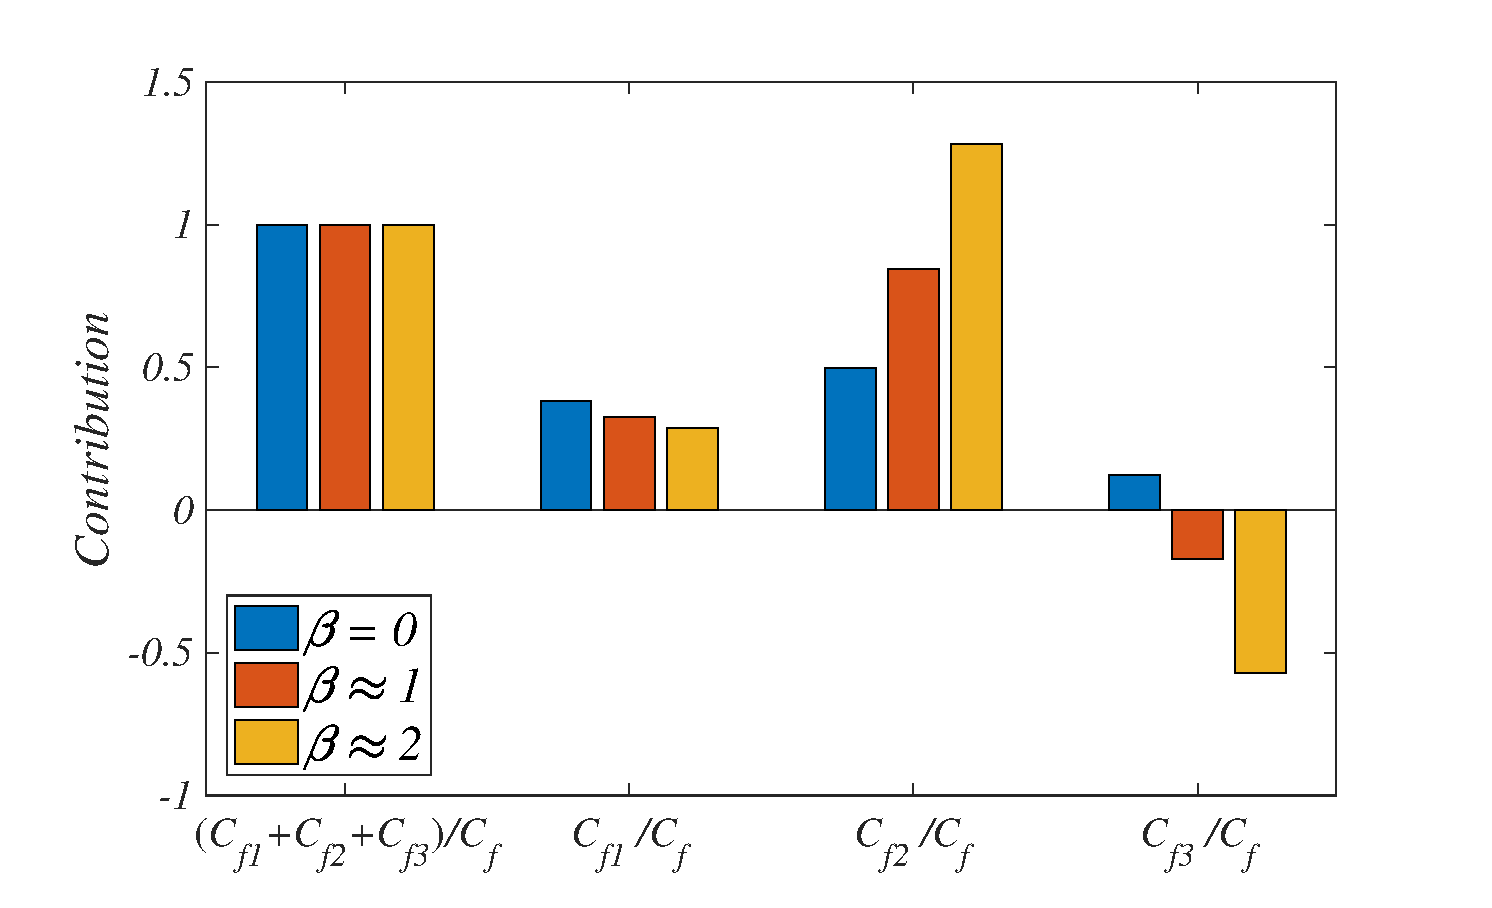
\includegraphics[width = 8cm]{1}}
\caption{Contributions of the three decomposed components for flat-plate TBLs with constant $\beta=0$, $\approx1$, and 2, and $Re_\tau=670$. }
\label{beta_cf}
\end{figure}

The ratios $C_{f1}/C_f$, $C_{f2}/C_f$, and $C_{f3}/C_f$ can be expressed as: 
\begin{eqnarray}
\frac{C_{f1}}{C_f}&=&\int_{0}^{Re_\tau}1/U_e^+\left(\frac{\partial \left<u\right>^+}{\partial y^+}\right)^2{\rm d}y^+,\label{cf1_cf}
\\
\frac{C_{f2}}{C_f}&=&\int_{0}^{Re_\tau}1/U_e^+\left<-u'v'\right>^+\frac{\partial \left<u\right>^+}{\partial y^+}{\rm d}y^+,\label{cf2_cf}
\\
\frac{C_{f3}}{C_f}&=&\int_{0}^{Re_\tau}1/U_e^+\left(\left<u\right>^+-U_e^+\right)\frac{\partial}{\partial y^+}\left(\frac{\partial \left<u\right>^+}{\partial y^+}-\left<u'v'\right>^+\right){\rm d}y^+,\label{cf3_cf}
\end{eqnarray}
where the superscript $+$ denotes normalization by local viscous units, i.e. friction velocity $u_\tau=\sqrt{(\tau_w/\rho)}$ and viscous length scale  $\delta_\nu=\nu/u_\tau$.

\begin{figure}
\subfigure{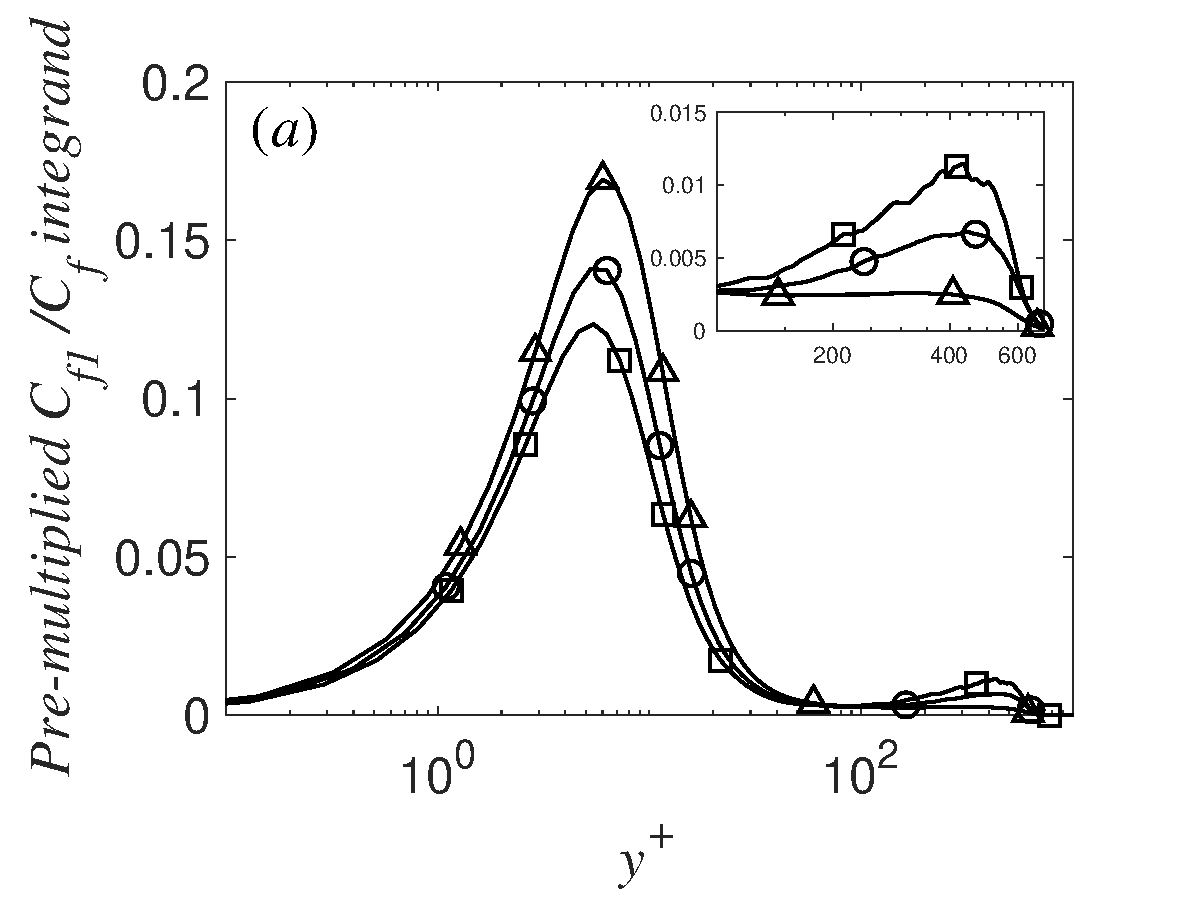
\includegraphics[width = 6cm]{2a}\label{beta1:a}}
\subfigure{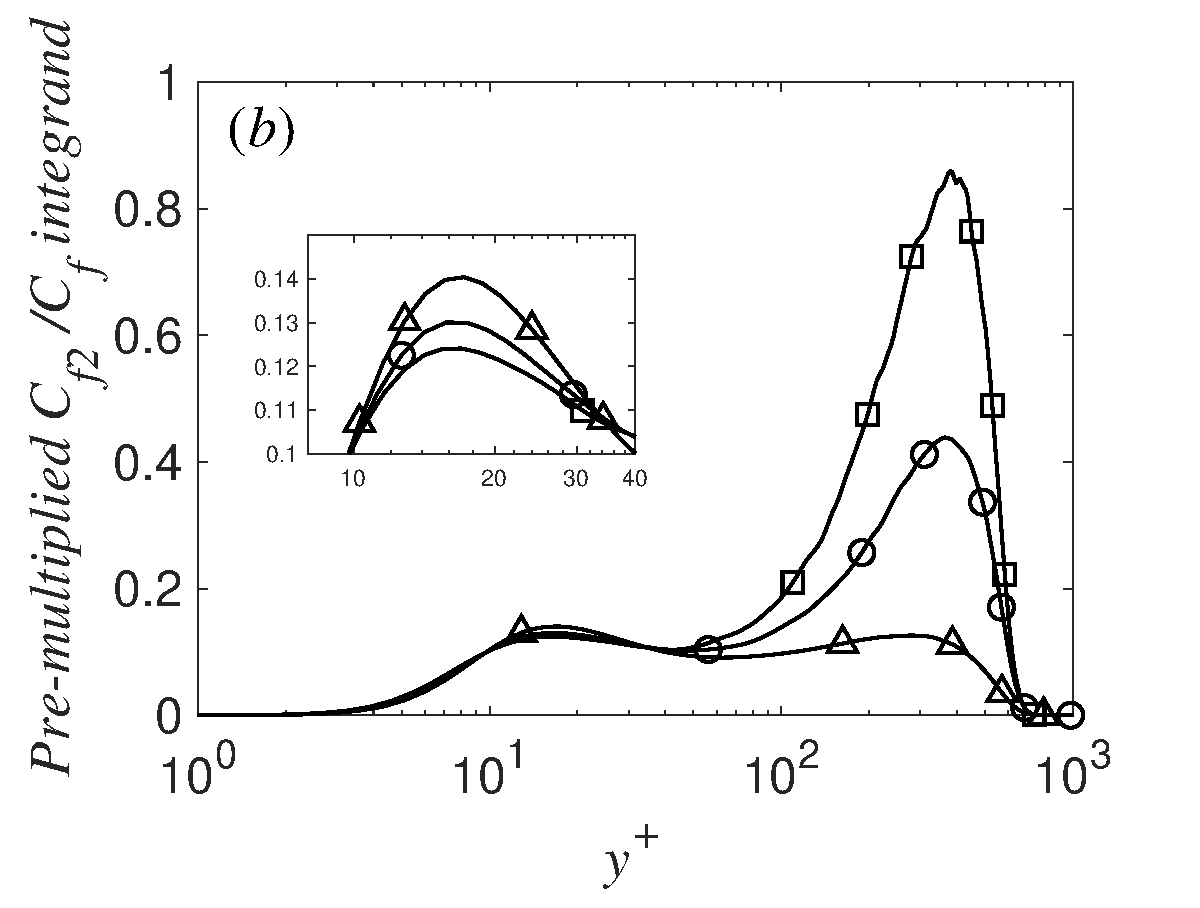
\includegraphics[width = 6cm]{2b}\label{beta1:b}}
\subfigure{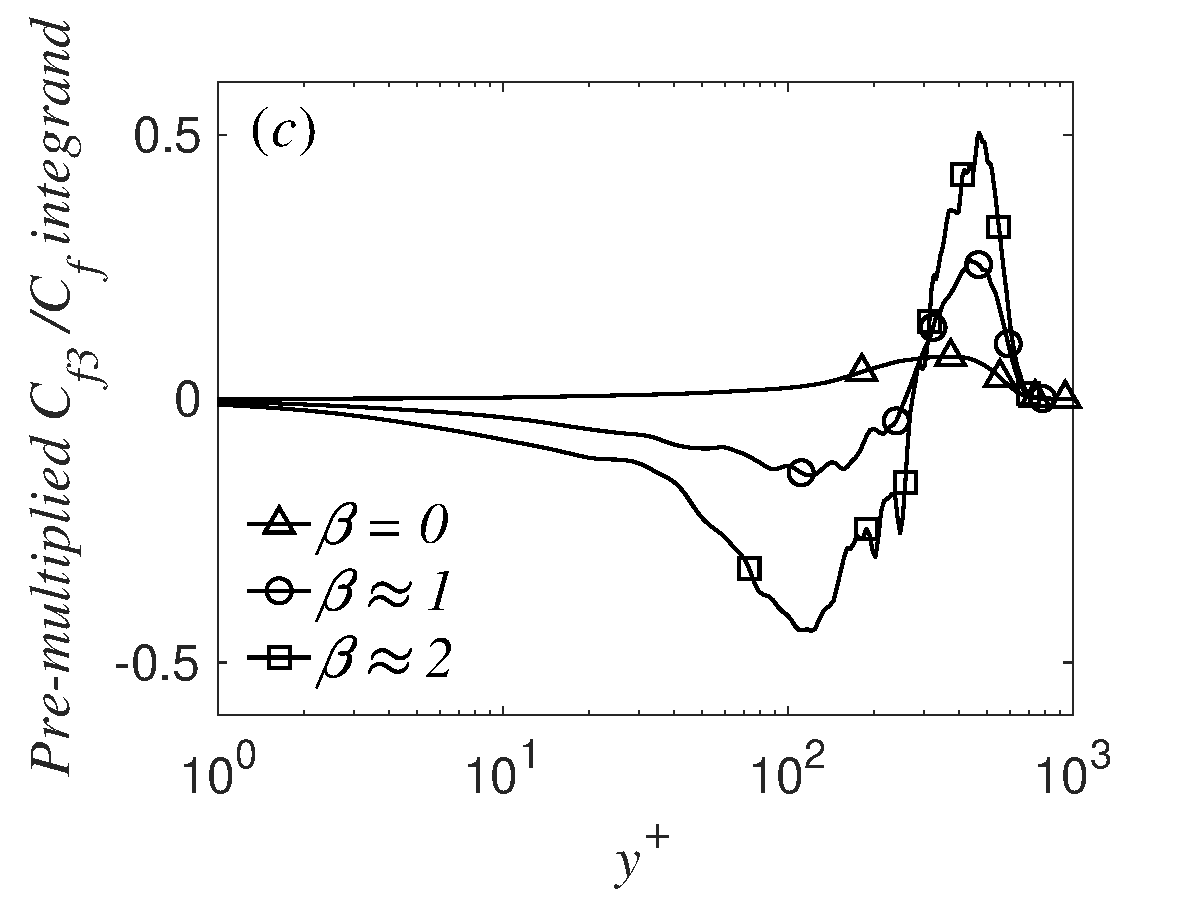
\includegraphics[width = 6cm]{2c}\label{beta1:c}}
\caption{Distributions of the pre-multiplied integrand in $C_{f1}/C_f$ ($a$), $C_{f2}/C_f$ ($b$), and $C_{f3}/C_f$ ($c$) as a function of $y^+$ for the flat-plate TBLs with constant $\beta=0$, $\approx1$, $\approx2$ and $Re_\tau=670$.}
\label{beta1}
\end{figure}


\begin{figure}
\subfigure{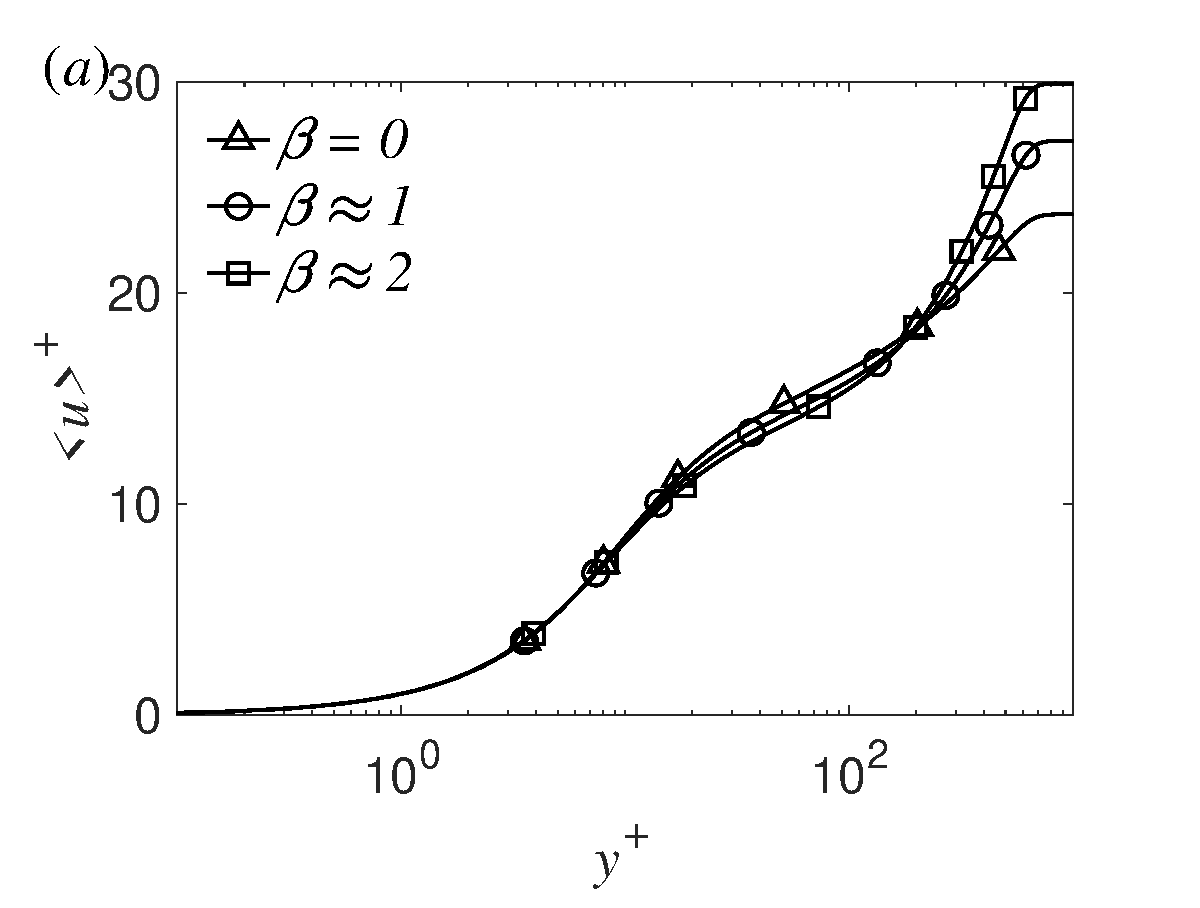
\includegraphics[width = 6cm]{3a}\label{prof:a}}
\subfigure{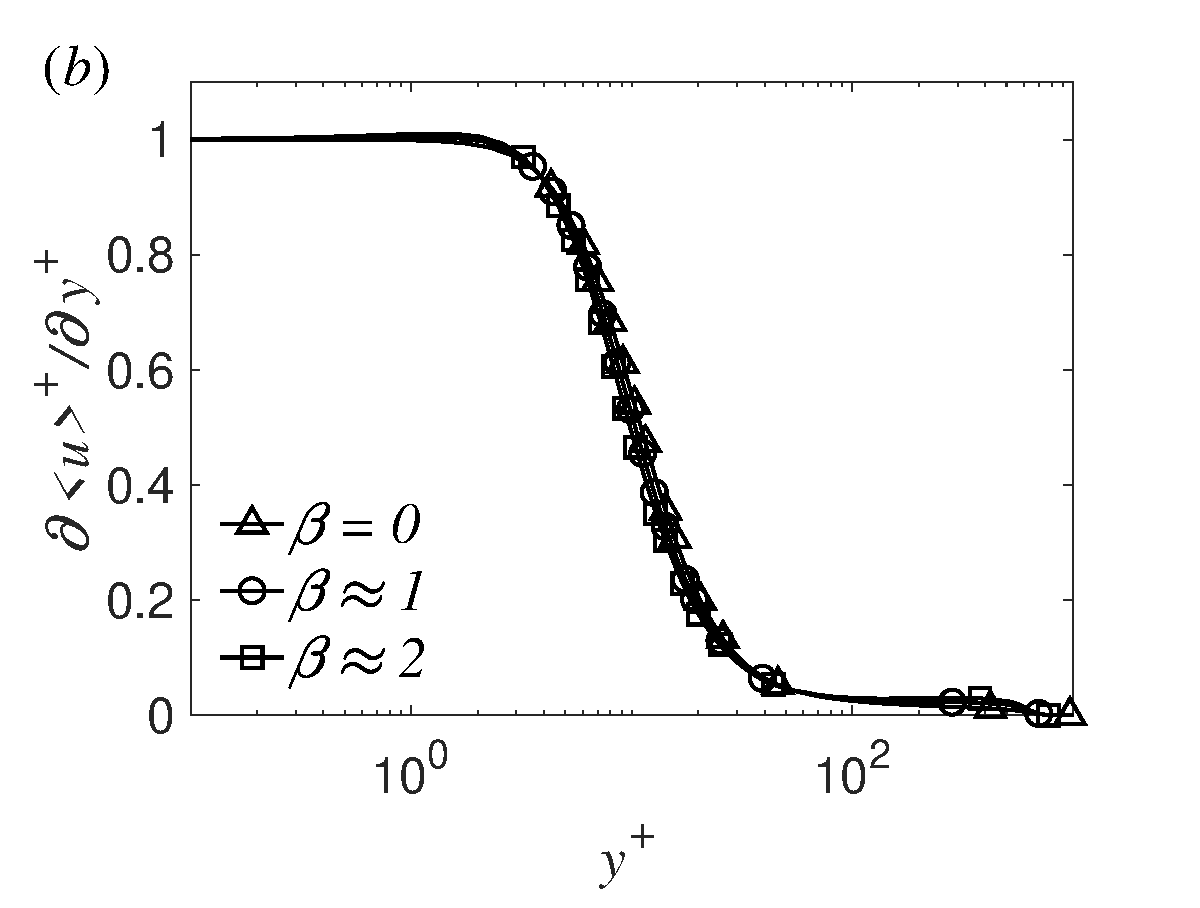
\includegraphics[width = 6cm]{3b}\label{prof:b}}
\subfigure{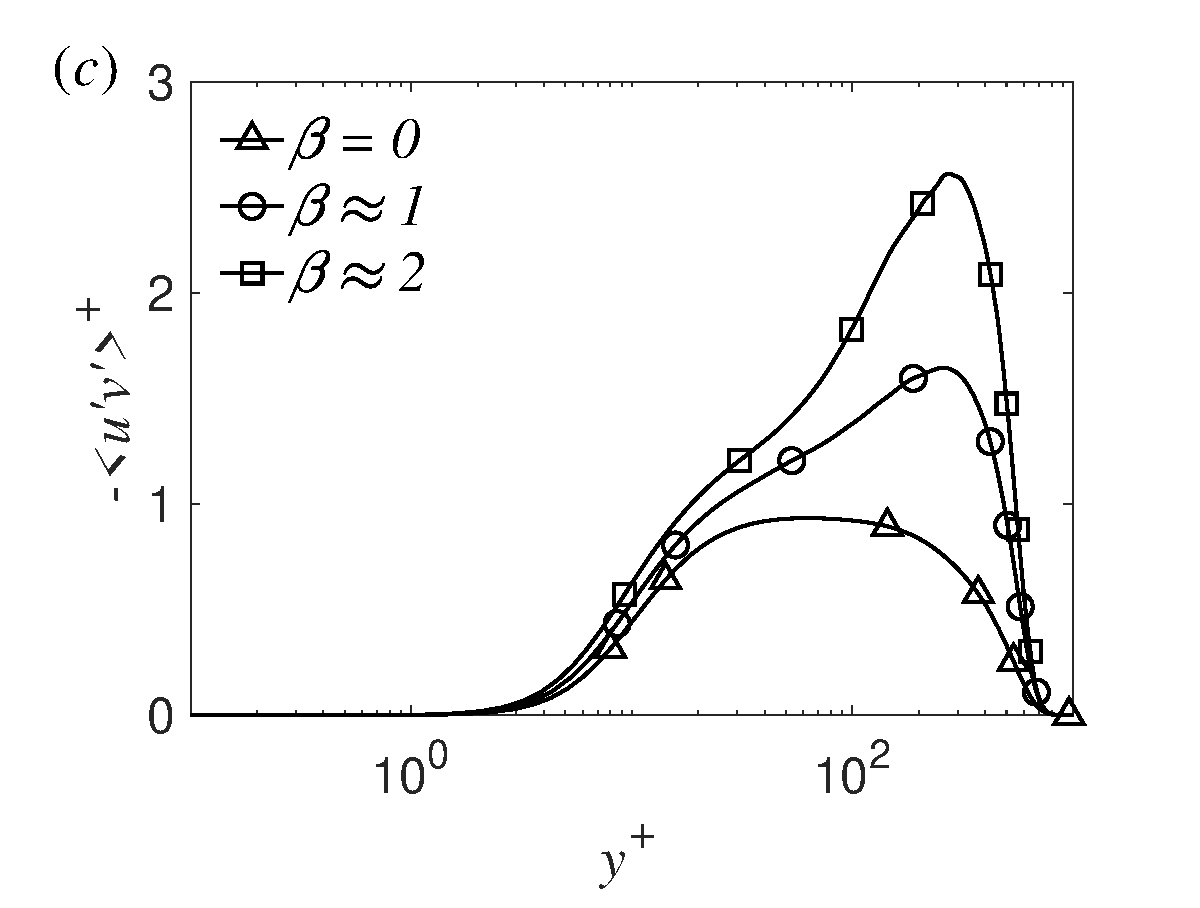
\includegraphics[width = 6cm]{3c}\label{prof:c}}
\subfigure{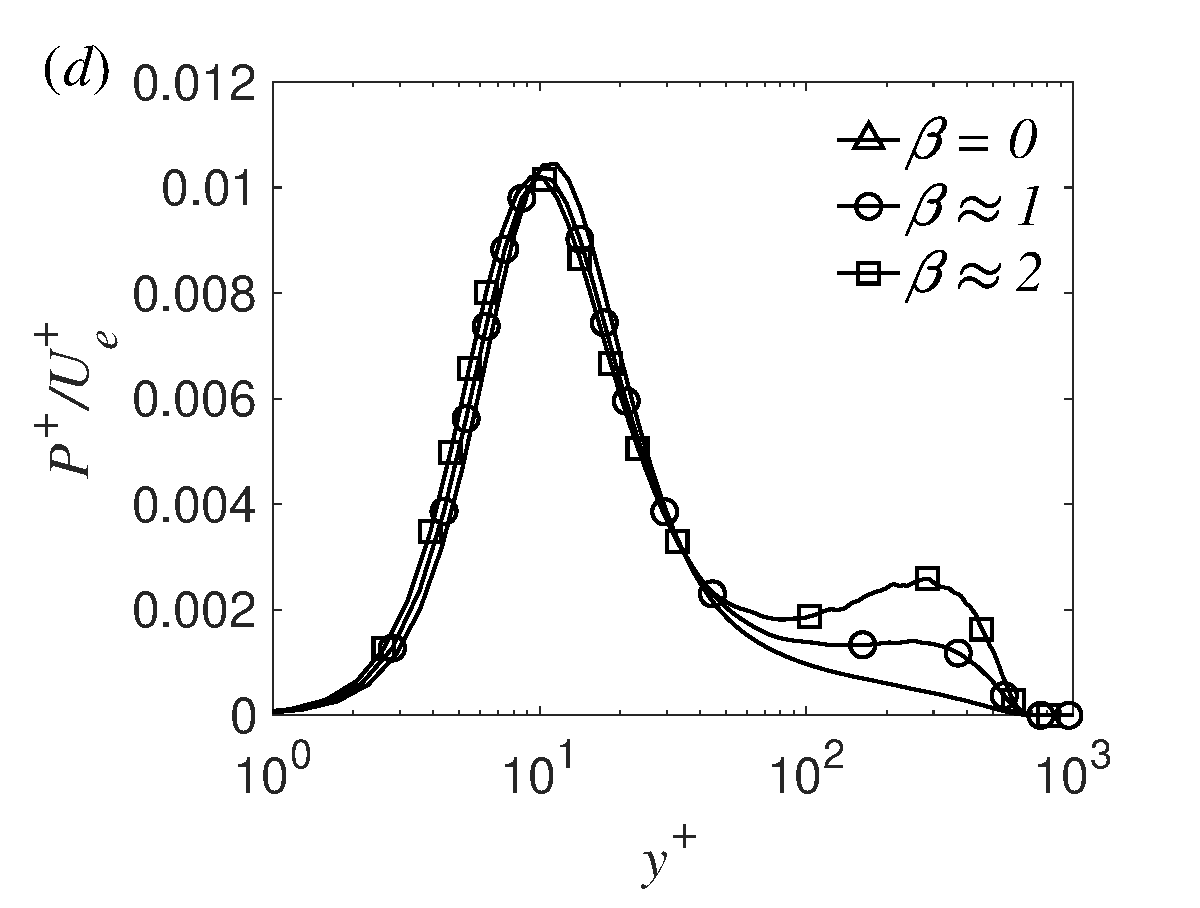
\includegraphics[width = 6cm]{3d}\label{prof:d}}
\caption{{\color{black}Profiles of mean streamwise velocity ($a$), wall-normal gradient of velocity ($b$), Reynolds shear stress ($c$), and production ($d$) as a function of $y^+$ for the flat-plate TBLs with constant $\beta=0$, $\approx1$, $\approx2$ and $Re_\tau=670$.}}
\label{prof}
\end{figure}


Wall-normal distributions of the pre-multiplied integrands in equations \eqref{cf1_cf}-\eqref{cf3_cf} are depicted in figure \ref{beta1}. The areas beneath the curves yield the proportion of $C_{f1}$, $C_{f2}$, and $C_{f3}$ with respect to the total, as displayed in figure~\ref{beta_cf}. It can be seen from figure \ref{beta1} that  for APG-TBLs, two peaks are observed respectively in the near-wall and outer regions both in the  distributions of $C_{f1}$-contribution and $C_{f2}$-contribution. 
Most of the $C_{f1}$-contributions come from the inner region ($y^+<30$), which is in line with the physics, i.e. the fact that the viscous dissipation is concentrated in the near-wall region\cite{Pope2000}. 
{\color{black}
As $\beta$ increases from 0 to 2, the inner-peak value is decreased, whereas its location remains fixed at $y^+ \approx 6.0$, which indicates that: 
\begin{equation}\label{eq:6}
\left.\begin{matrix}
\frac{{\rm d} \left[{y^+(\partial\left<u\right>^+/\partial y^+)^2}\right]}{{\rm d} y^+} 
\end{matrix}\right|_{y^+\approx6} =0.
\end{equation}
This differential equation finally yields:
\begin{equation}\label{eq:7}
\left.\begin{matrix}
\frac{{\rm d} \ln \left({{\rm d} \left<u\right>^+}/{{\rm d} y^+}\right)}{{\rm d} \ln y^+}
\end{matrix}\right|_{y^+\approx6}=-\frac{1}{2},
\end{equation}
leading to a local expansion of $\left<u\right>^+-\left<u\right>^+\mid_{y^+\approx6} \propto \left (y^{+}\right)^{1/2}$ at $y^+\approx6$, regardless of the imposed pressure gradient.
This phenomenon is interesting, extending our knowledge on the mean velocity profile beyond the viscous sublayer (up to $y^+=5$).
}
Meanwhile, as shown in the inset of figure \ref{beta1:a}, a small secondary peak appears in the outer region of APG-TBLs, and the peak value is increased with $\beta$. 
Note that this secondary peak is absent in the ZPG-TBLs, even at higher Reynolds numbers up to $Re_\tau=1270$\cite{Fan2019}. This suggests that the APG has an action to enhance the generation of outer-layer energy, which is consistent with the observation in the studies by \citet{Tanarro2020} and \citet{Vila2020}.


As for the $C_{f2}$-contributions shown in figure \ref{beta1:b}, {\color{black}they are related to  the distribution of pre-multiplied production $P^+$\cite{Smits2011}, which is defined as $P^+=\left<-u'v'\right>^+ {{\rm d} \left<u\right>^+}/{{\rm d} y^+}$; thus the $C_{f2}$-contributions correspond to $y^+P^+/U_e^+$.} Note that two peaks are observed in the inner and outer regions located at $y^+\approx16.5$ and $y^+\approx300-400$, respectively. {\color{black}
The inner-layer peak collapse at $y^+\approx16.5$ indicates that:
\begin{equation}
\left.\begin{matrix}
\frac{{\rm d} ({y^+P^+})}{{\rm d} y^+}
\end{matrix}\right|_{y^+\approx16.5}=0,
\end{equation}
suggesting that the trend $P^+ \propto 1/y^+$ holds at $y^+\approx16.5$.
}
{\color{black}
For increasing $\beta$, the inner peak decreases, while the outer peak increases dramatically and becomes dominant in the $C_{f2}$-contributions, which is ascribed to the remarkable upward shift of the mean velocity and Reynolds shear stress in the wake region, as shown in figure~\ref{prof}. Thus, in contrast to ZPG-TBLs, outer-layer motions carry larger amounts of turbulence kinetic energy in APG-TBLs, which were found to be associated with the energisation of large-scale structures\cite{Harun2013,Lee2017,Kitsios2017,Lee2008,Vinuesa2018}.}
%Previous studies\cite{Harun2013,Lee2017,Kitsios2017} have reported that the large peak of turbulence kinetic energy production in the outer region of APG-TBLs \cite{Lee2008} is caused by the energisation of large-scale outer motions.
Consequently, as for the mean friction generation, the large $C_{f2}$-contributions observed in the outer region are directly linked to the energisation of large-scale motions, especially for the APG-TBLs with high $\beta$. 
{\color{black}
Note that $y^+P^+$ defines the log density of production.
Its good collapse at $y^+\approx16.5$ does not mean that the peak location of $P^+$ also keeps invariant. As shown in figure~\ref{prof:d}, the inner-peak locations of $P^+$ are shifted closer to the wall in viscous units as $\beta$ increases ($P^+/U_e^+$ in figure~\ref{prof:d} is exactly the integrand of $C_{f2}/C_f$, and the prefactor of $1/U_e^+$ will not influence the peak locations.).
}

Things are quite different for the $C_{f3}$-contributions, as shown in figure~\ref{beta1:c}: in ZPG-TBLs, the $C_{f3}$-contributions are always positive;
%, which is ascribed to the negative convection term $\left(\left<u\right>{\partial\left<u\right>}/{\partial x}+\left<v\right>{\partial\left<u\right>}/{\partial y}\right)$ \cite{Fan2019} across the entire wall layer (see equation (2) in \citet{Fan2019})
on the other hand, in the APG-TBLs, negative $C_{f3}$-contributions are observed within $y^+\lesssim300$, and positive values beyond this region. According to equation \eqref{cf3}, $C_{f3}$ consists of three parts: convection term ($C_{f31}$), streamwise-heterogeneity term ($C_{f32}$), and pressure-gradient term ($C_{f33}$), and their ratios with respect to $C_f$ can be written as:
\begin{eqnarray}
\frac{C_{f31}}{C_f}&=&1/U_e^+\int_{0}^{Re_\tau}(\left<u\right>^+-U_e^+)\left(\left<u\right>^+\frac{\partial\left<u\right>^+}{\partial x^+}+\left<v\right>^+\frac{\partial\left<u\right>^+}{\partial y^+}\right) {\rm d}y^+,\label{cf31_cf}\\
\frac{C_{f32}}{C_f}&=&1/U_e^+\int_{0}^{Re_\tau}-(\left<u\right>^+-U_e^+)\left( \frac{\partial^2\left<u\right>^+}{\partial x^{+2}}-\frac{\partial\left<u'u'\right>^+}{\partial x^+}\right) {\rm d}y^+,\label{cf32_cf}\\
\frac{C_{f33}}{C_f}&=&1/{U_e^+}\int_{0}^{Re_\tau}(\left<u\right>^+-U_e^+)\left(\frac{{\rm d}  p/(\rho u_\tau^2)}{{\rm d}  x^+}\right) {\rm d}y^+.\label{cf33_cf}
\end{eqnarray}
Figure~\ref{beta_cf3} shows the wall-normal distributions of the pre-multiplied integrands in equations~\eqref{cf31_cf}--\eqref{cf33_cf}.
The $C_{f31}$-contributions are always positive and mainly confined to the outer region. Its peak value is significantly increased with APG magnitude, which is in accordance with stronger outer-layer convection at higher $\beta$. The effect of streamwise heterogeneity, as shown in figure~\ref{beta_cf3:b}, is negligible due to its small amplitude. 
%{\color{black}Wrinkles in figure~\ref{beta_cf3:a} and \ref{beta_cf3:b} are caused by the calculations of streamwise derivatives.}
With the imposed adverse pressure gradients, negative $C_{f33}$-contributions are observed across the boundary layer, as expected, as shown in figure \ref{beta_cf3:c}. Thus, the sign switching of the $C_{f3}$-contributions in figure~\ref{beta1:c} is mainly related to the counterbalance between the convection term ($C_{f31}$) and the pressure-gradient term ($C_{f33}$).


%\textcolor{red}{Maybe delete this part???} At last, we sum up $C_{f1}/C_f$, $C_{f2}/C_f$ and $C_{f3}/C_f$ and give its wall-normal distributions in figure \ref{sum}. the remarkable contribution of the outer-layer dynamics is observed at high $\beta$. Adverse pressure gradient significantly weakens the role of turbulence dynamics in the generation of skin friction within the range up to $y^+\approx200$, which could possibly lead to a decrease in the efficiency of friction reduction strategies based on near-wall controls in the APG-TBLs.





\begin{figure}
\subfigure{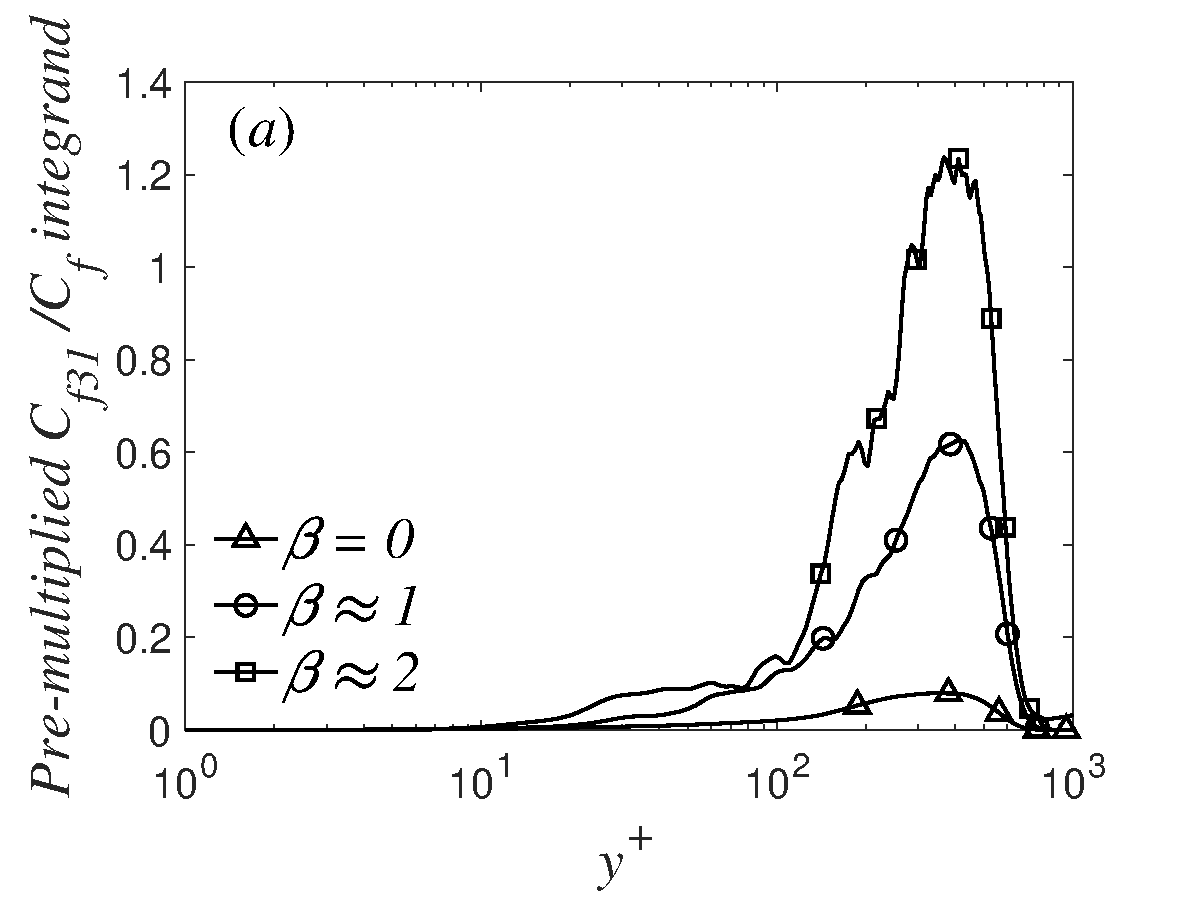
\includegraphics[width = 6cm]{4a}\label{beta_cf3:a}}
\subfigure{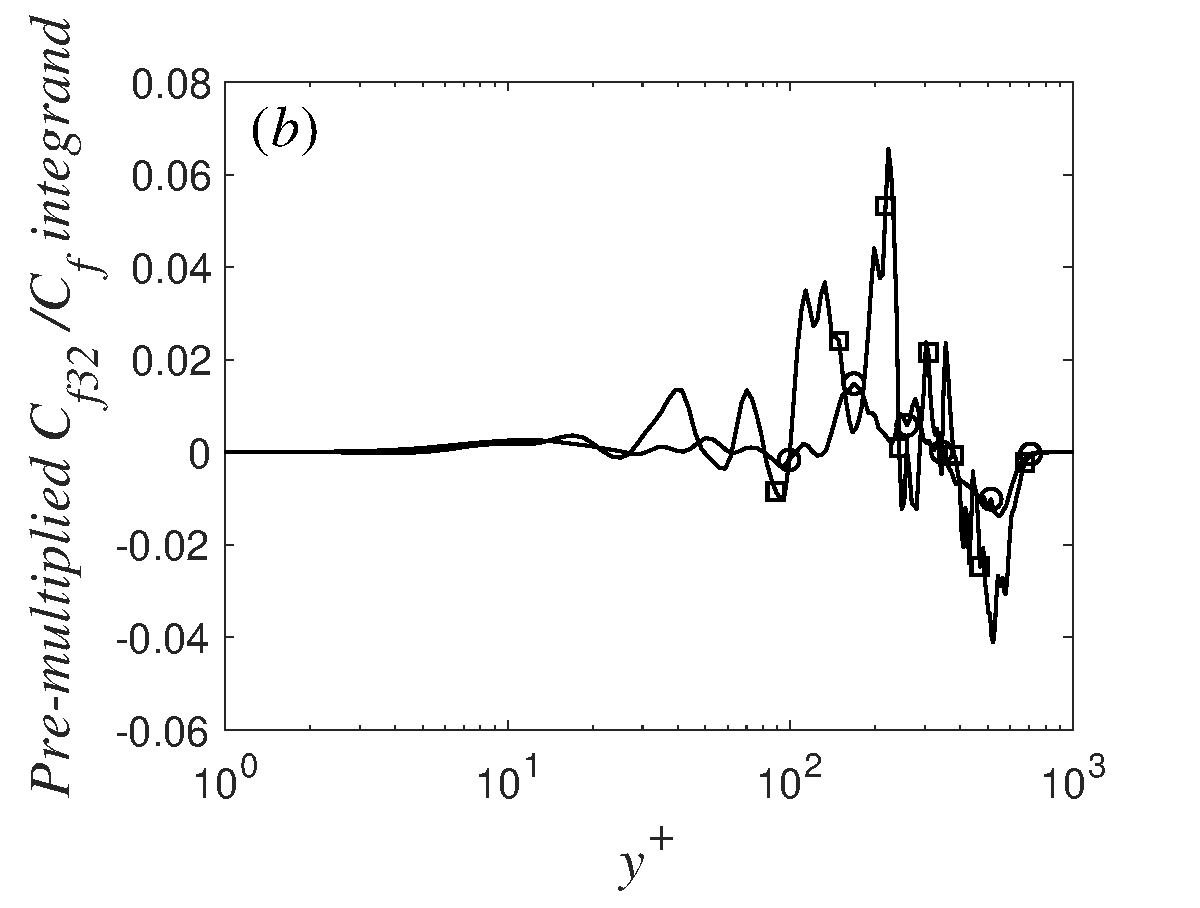
\includegraphics[width = 6cm]{4b}\label{beta_cf3:b}}
\subfigure{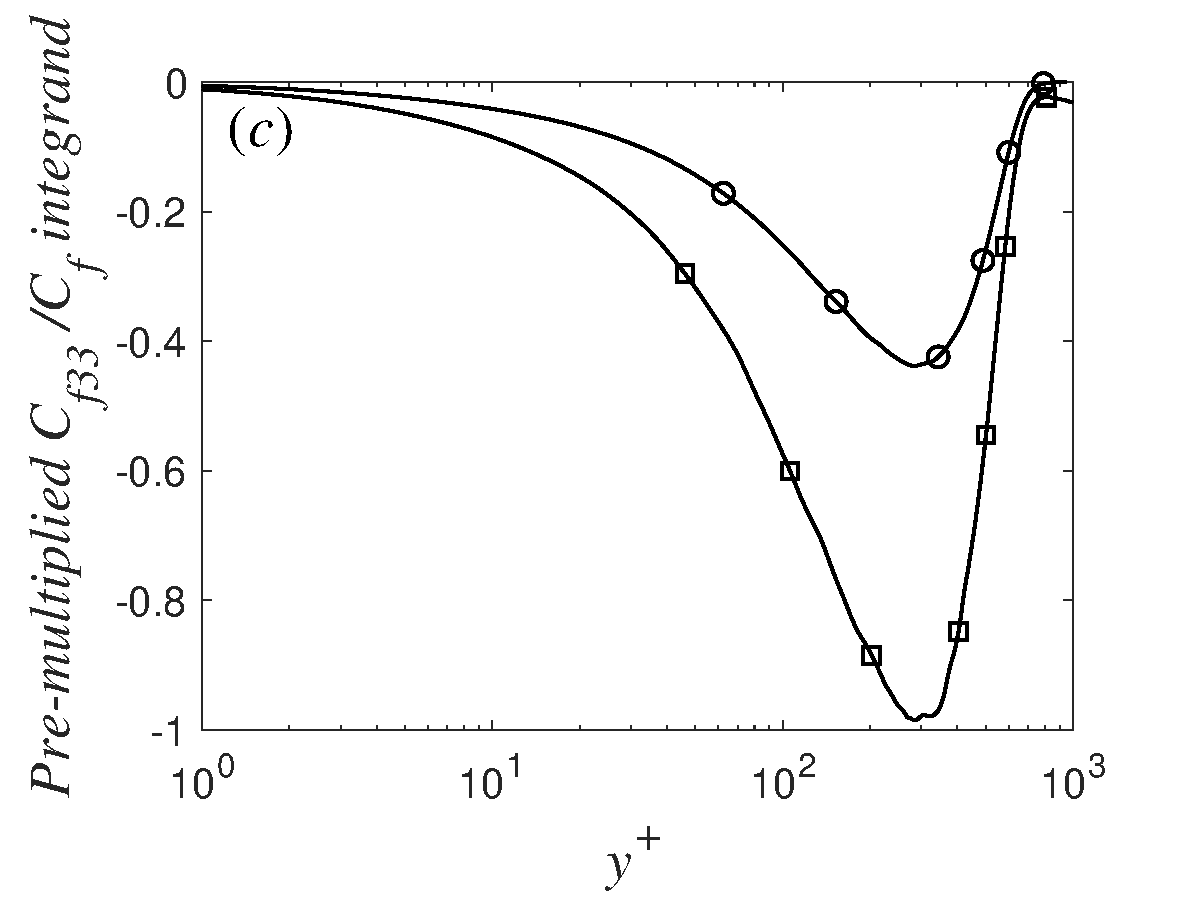
\includegraphics[width = 6cm]{4c}\label{beta_cf3:c}}
\caption{Distributions of the pre-multiplied integrand in $C_{f31}/C_f$ ($a$), $C_{f32}/C_f$ ($b$), and $C_{f33}/C_f$ ($c$) as a function of $y^+$ for the flat-plate TBLs with constant $\beta=0$, $\approx1$, $\approx2$ and $Re_\tau=670$.}
\label{beta_cf3}
\end{figure}

%\begin{figure}
%\includegraphics[width = 7.5cm]{fig/sum}
%\caption{The distributions of the pre-multiplied integrand in $(C_{f1}/C_f+C_{f2}/C_f+C_{f3}/C_f)$ as a function of $y^+$ for the TBLs at $\beta=0$, $\approx1$, $\approx2$ and $Re_\tau=670$.}
%\label{sum}
%\end{figure}
%

\subsection{Reynolds-number effects on the various terms}\label{Re-eff}
After assessing the impact of the APG magnitude on the $C_f$ decomposition terms for fixed $Re_{\tau}$, here we analyze their evolution with Reynolds number for approximately constant $\beta$. For this analysis we consider an APG-TBL database with $\beta\approx1.4$ and $Re_\tau$ ranging from 1000 to 2000, the wall-normal distributions of the pre-multiplied integrands in equations \eqref{cf1_cf}-\eqref{cf3_cf} are shown in figure~\ref{reys}. Similar features can be found in the APG-TBLs with $\beta\approx 1$ and 2 (see Appendix~\ref{app1}). As depicted in figures \ref{reys:a} and \ref{reys:b}, the inner peaks of the $C_{f1}$- and $C_{f2}$-contributions are fixed at $y^+\approx6$ and $y^+\approx16.5$, respectively.
Meanwhile, secondary peaks appear both in the $C_{f1}$- and $C_{f2}$-contributions, which are associated with the enhancement of outer-layer energy.
%small- and large-scale motions populating in the outer region, respectively.
{\color{black}
In outer scaling, i.e. in terms of $\delta_{99}$, as depicted in figure \ref{reys:d}, the secondary peaks of the $C_{f1}$- contributions collapse well at $y/\delta_{99}\approx0.7$. Similar to the feature of mean velocity profile in the vicinity of $y^+\approx6$ (as interpreted with equations~\eqref{eq:6}-\eqref{eq:7}), the secondary peak indicates that ${\rm d} [{y({\rm d}\left<u\right>/{\rm d} y)^2}]/{\rm d} (y/\delta_{99})|_{y/\delta_{99}\approx0.7}=0$, suggesting a local expansion of mean velocity profile near $y/\delta_{99}\approx0.7$, i.e. 
$\left<u\right>-\left<u\right>\mid_{y/\delta_{99}\approx0.7}\propto (y/\delta_{99})^{1/2}$.
As for the secondary peaks of the $C_{f2}$-contributions, they are perfectly collapsed at $y/\delta_{99}\approx0.53$ (as shown in figure \ref{reys:e}), revealing a local feature of the production ($P$) distribution, that is $P\mid_{y/\delta_{99}\approx0.53}\propto1/(y/\delta_{99})$.}
%{\color{black}Whereas the outer peak values decrease with Reynolds number increasing, suggesting that higher-Re TBLs are less sensitive to APG effects, consistent with the conclusion in \citet{Vinuesa2018}.}
These features are also confirmed in the APG-TBLs developing on the NACA4412 wing section, subjected to much higher APG magnitudes, {\color{black}which indicates that the outer-peak locations are well-collapsed regardless of pressure-gradient magnitude as well,} as discussed in the following subsection.



The wall-normal distribution of the pre-multiplied integrand in $C_{f3}/C_f$ (figures~\ref{reys:c} and \ref{reys:f}) shows that both the valley and peak locations appear to be well-scaled by outer units. The valleys collapse at $y/\delta_{99}\approx0.1$, and the peaks at $y/\delta_{99}\approx0.65$.
It is reasonable that both the convection ($C_{f31}/C_f$) and pressure-gradient term ($C_{f33}/C_f$) are dominated by large-scale motions. 
{\color{black}
As the Reynolds number increases, both the absolute values of the valley and peak decrease. To clarify this variation, we trace back to the profile of mean convection in the momentum-balance equation (i.e. $( \left<u\right>{\partial\left<u\right>}/{\partial x}+\left<v\right>{\partial\left<u\right>}/{\partial y})/(U_e^2/\delta_{99})$ ). As shown in figure \ref{conv}, the mean convection decreases with $Re_\tau$, supporting that the increasing Reynolds number could attenuate the effects caused by the adverse pressure gradient in the wake region. This is an agreement with previous APG-TBL studies\cite{Vinuesa2018}.
}


%related to the weakened convection and ${\rm d}p/{\rm d}x$ within the boundary layer. 
%Note that this decreasing trend may not be much evident here due to the limited range of Reynolds number, however can be further confirmed in the following cases of NACA0012.



\begin{figure}[htb]
\subfigure{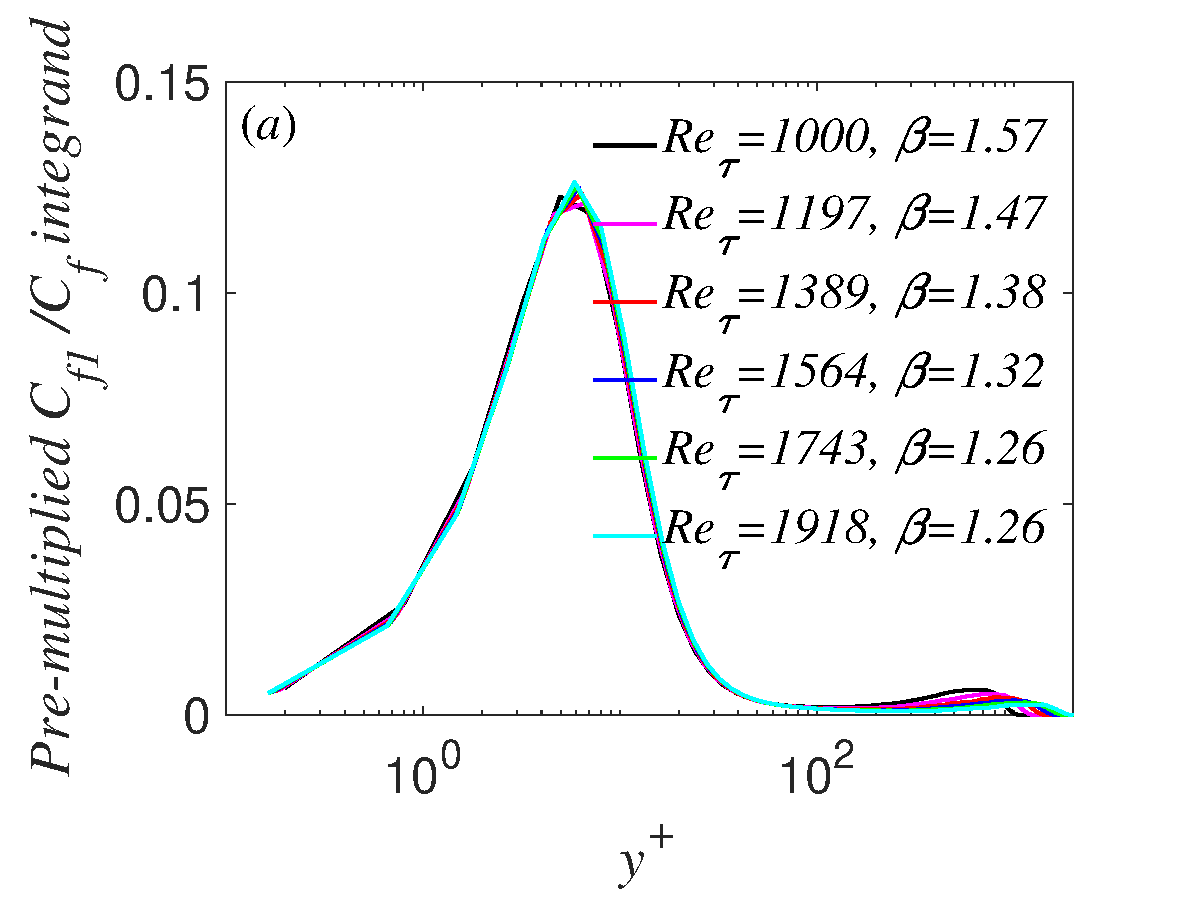
\includegraphics[width = 6cm]{5a} \label{reys:a}}
\subfigure{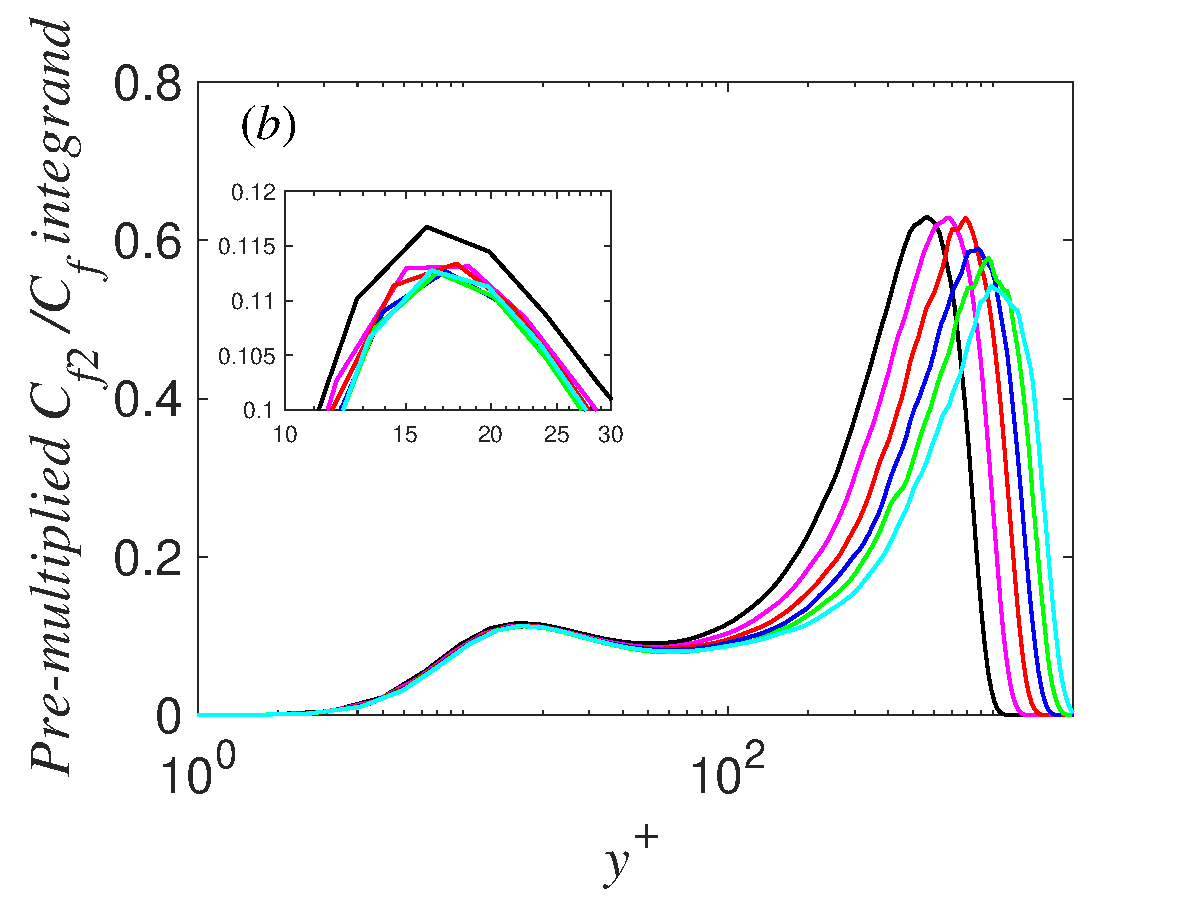
\includegraphics[width = 6cm]{5b} \label{reys:b}}
\subfigure{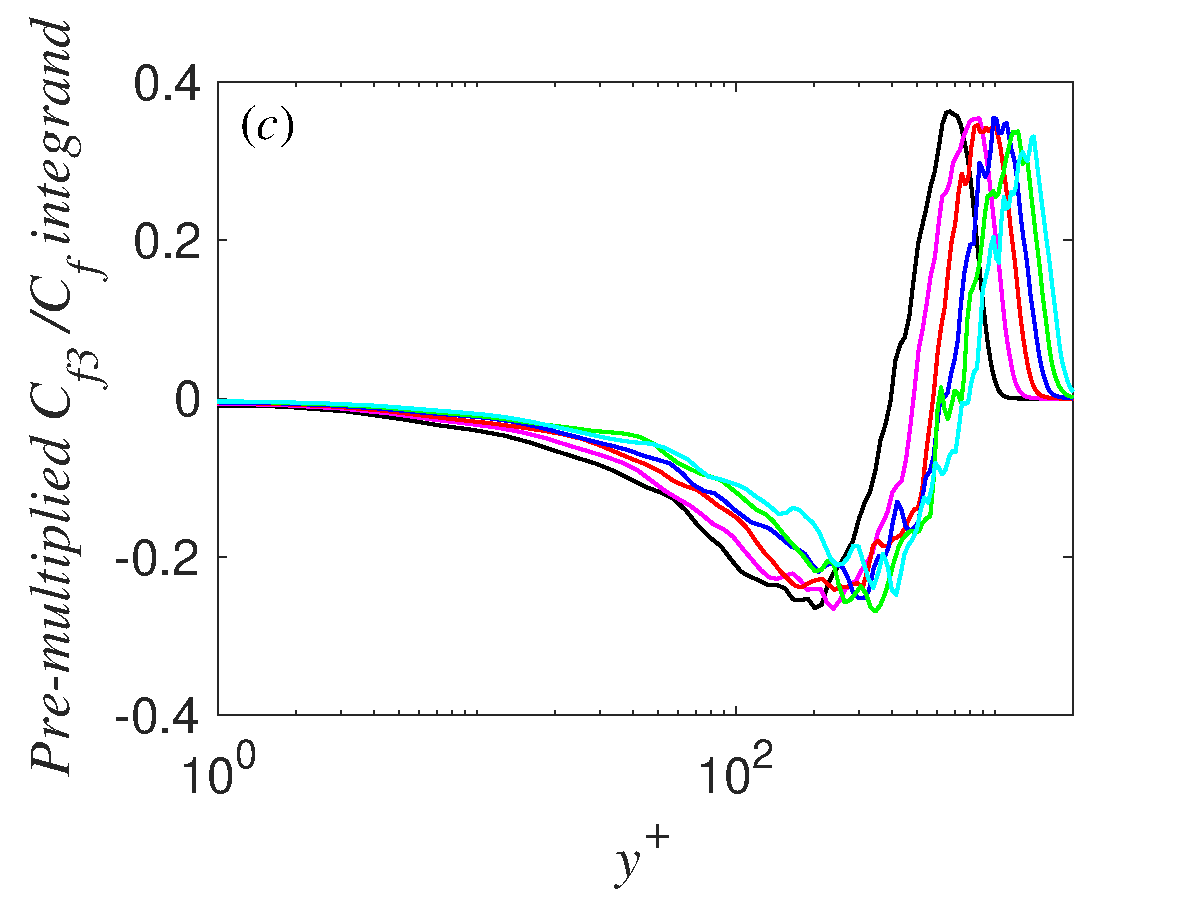
\includegraphics[width = 6cm]{5c} \label{reys:c}}
\subfigure{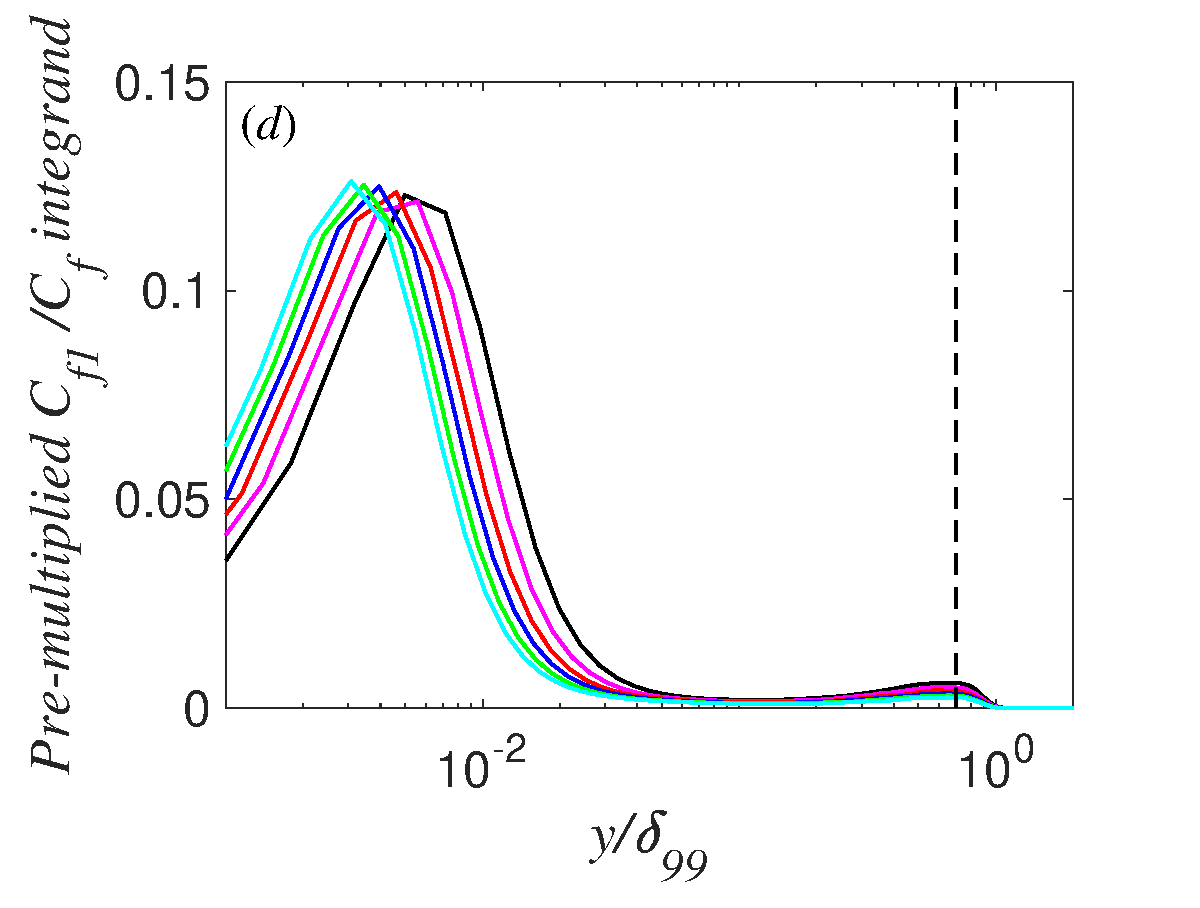
\includegraphics[width = 6cm]{5d} \label{reys:d}}
\subfigure{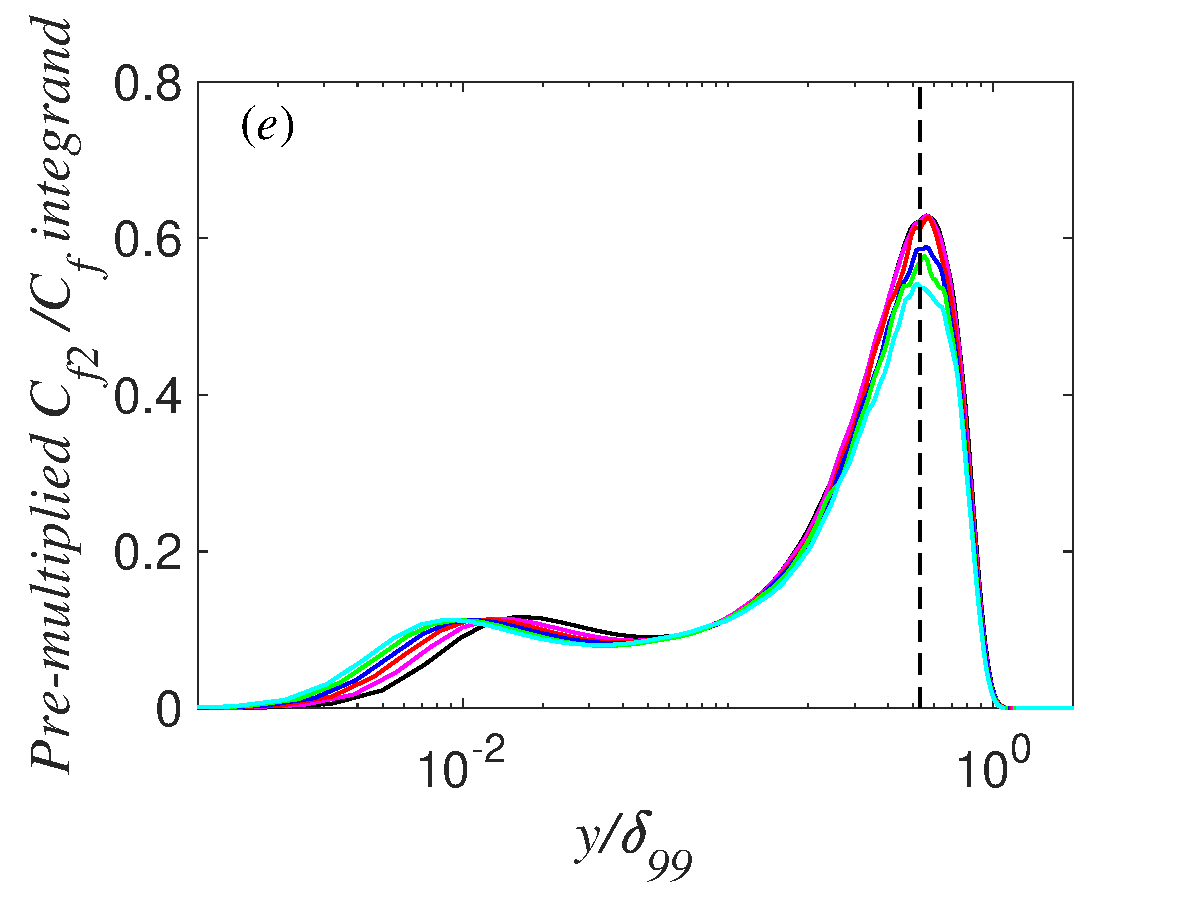
\includegraphics[width = 6cm]{5e} \label{reys:e}}
\subfigure{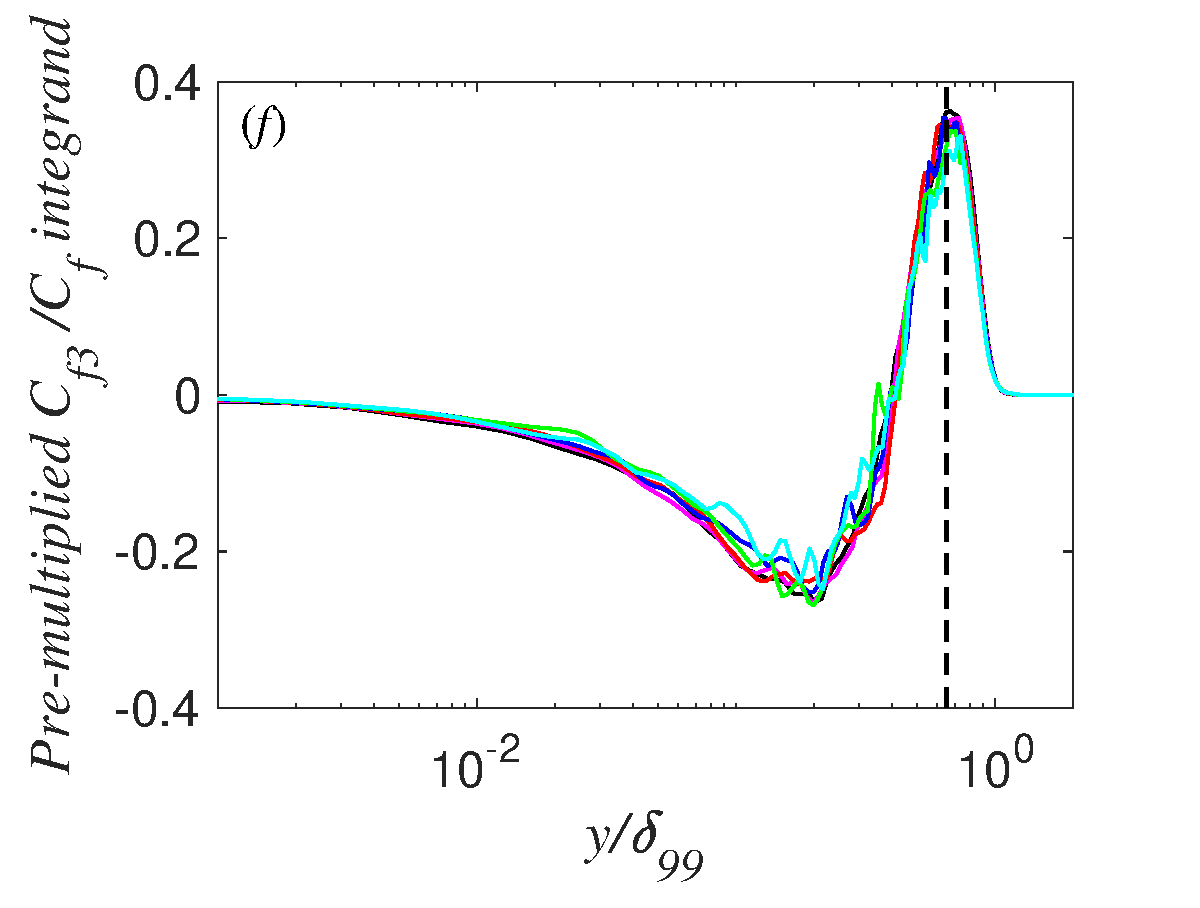
\includegraphics[width = 6cm]{5f} \label{reys:f}}
\caption{Distributions of the pre-multiplied integrand in $C_{f1}/C_f$, $C_{f2}/C_f$, and $C_{f3}/C_f$ as a function of $y^+$ ($a$--$c$) and as a function of  $y/\delta_{99}$  ($d$--$f$)  for the APG-TBL with $\beta\approx1.4$. The vertical dashed lines in ($d$--$f$) mark the position $y/\delta_{99}=0.7$, 0.53, and 0.65 respectively.}
\label{reys}
\end{figure}


\begin{figure}
\centering
\subfigure{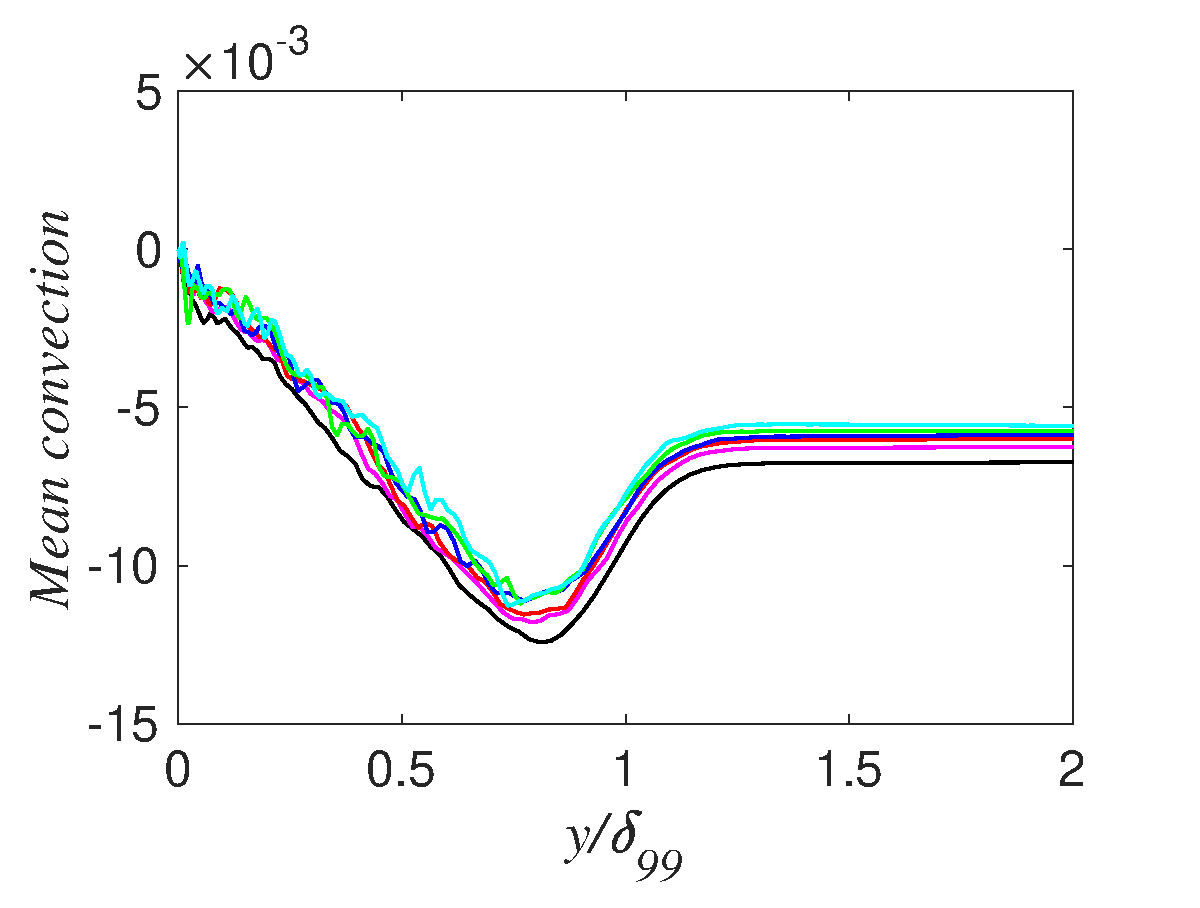
\includegraphics[width = 8cm]{6}}
\caption{{\color{black}Profiles of mean convection $(\left<u\right>{\partial\left<u\right>}/{\partial x}+\left<v\right>{\partial\left<u\right>}/{\partial y})/(U_e^2/\delta_{99})$ for the APG-TBL with $\beta\approx1.4$. For legends, see caption in figure \ref{reys}.}}
\label{conv}
\end{figure}

{\color{black}
Finally, the well-collapsed outer-peak locations in figure~\ref{reys}($d$-$f$) can be related to the mean streamwise kinetic energy budget equation:
\begin{equation}\label{eq:12}
\frac{\partial}{\partial y}\left[\left(\left<u\right>-U_e\right)\frac{\tau}{\rho}\right]=\nu\left(\frac{\partial\left<u\right>}{\partial y}\right)^2+\left<-u'v'\right>\frac{\partial\left<u\right>}{\partial y}+\left(\left<u\right>-U_e\right)\frac{\partial\tau/\rho}{\partial y},
\end{equation}
where $\tau/\rho=\nu\partial\left<u\right>/\partial y-\left<u'v'\right>$. The term on the left-hand side of equation~\eqref{eq:12} represents the power of viscous and turbulent stresses, and the terms on the right-hand side represent viscous dissipation, turbulence kinetic energy production, and spatial growth, respectively. Their pre-multiplied distributions are plotted in figure~\ref{balan}. Similarity of outer-layer peak locations is obvious, and distributions of dissipation, production, and spatial growth are balanced by the power done by total shear stress in each layer.


\begin{figure}
\subfigure{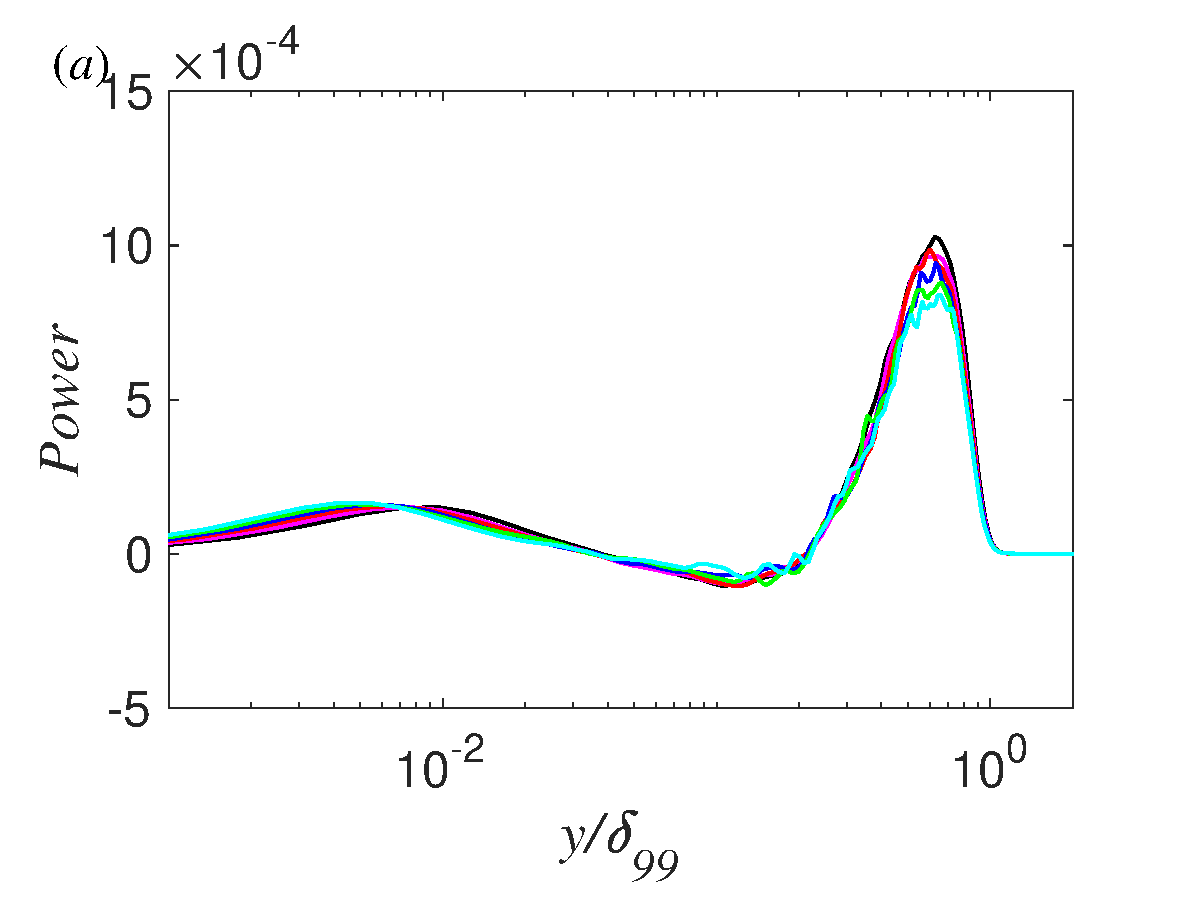
\includegraphics[width = 6cm]{7a}\label{balan:a}}
\subfigure{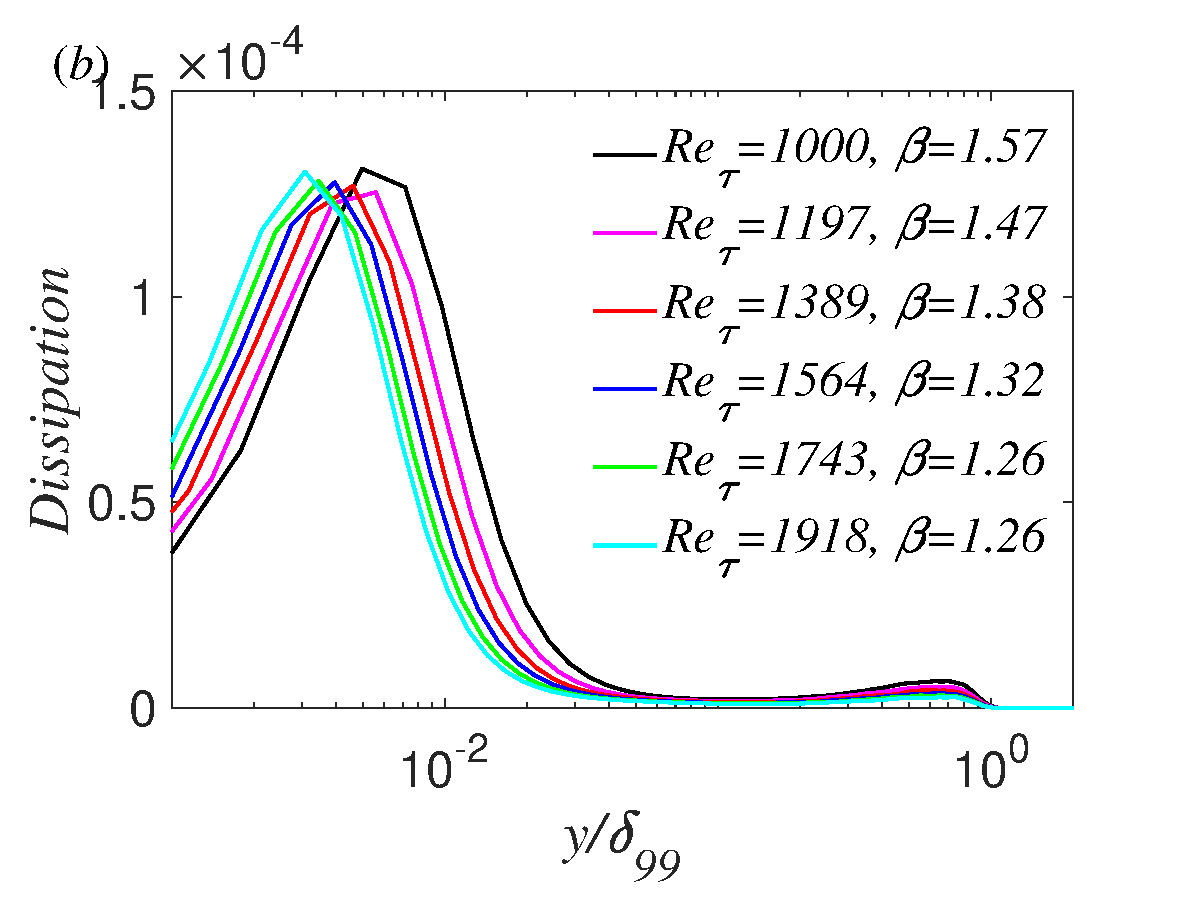
\includegraphics[width = 6cm]{7b}\label{balan:b}}
\subfigure{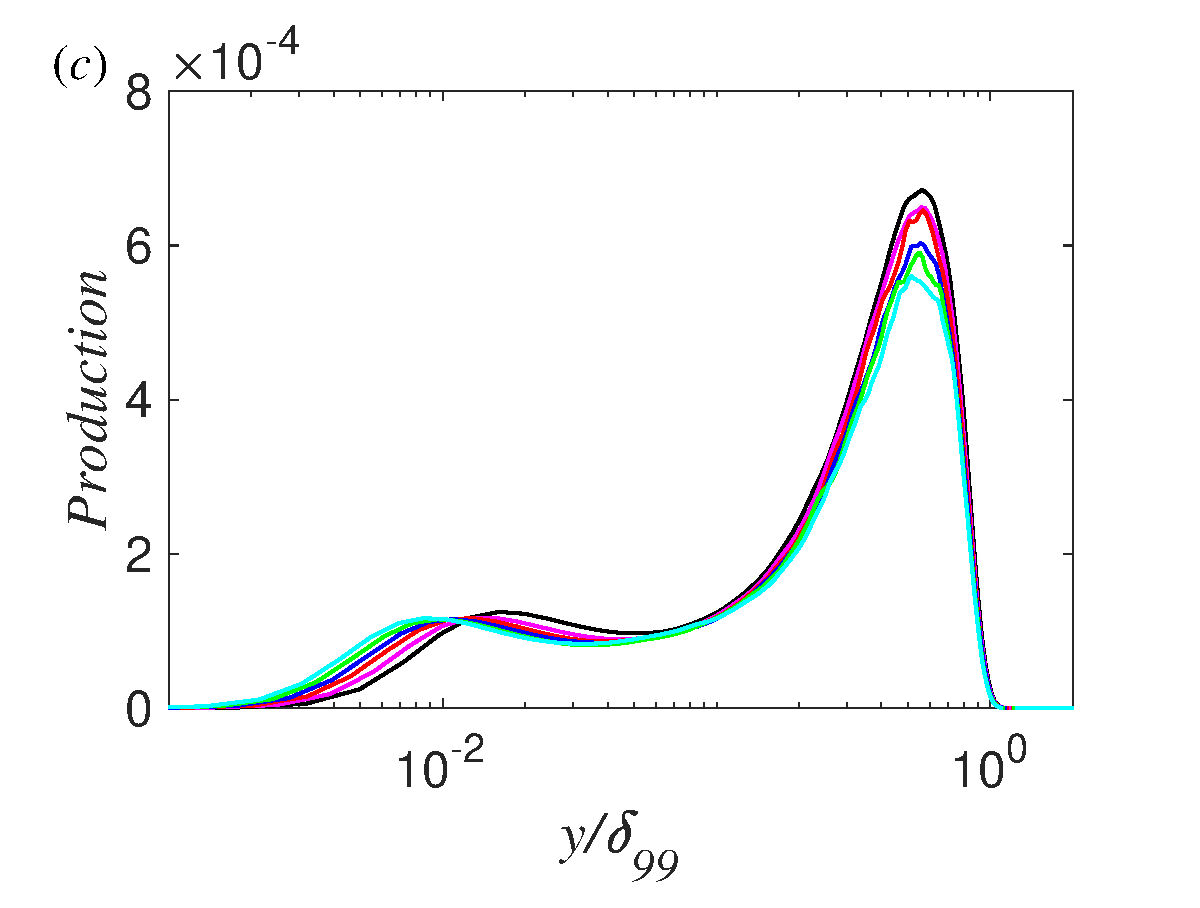
\includegraphics[width = 6cm]{7c}\label{balan:c}}
\subfigure{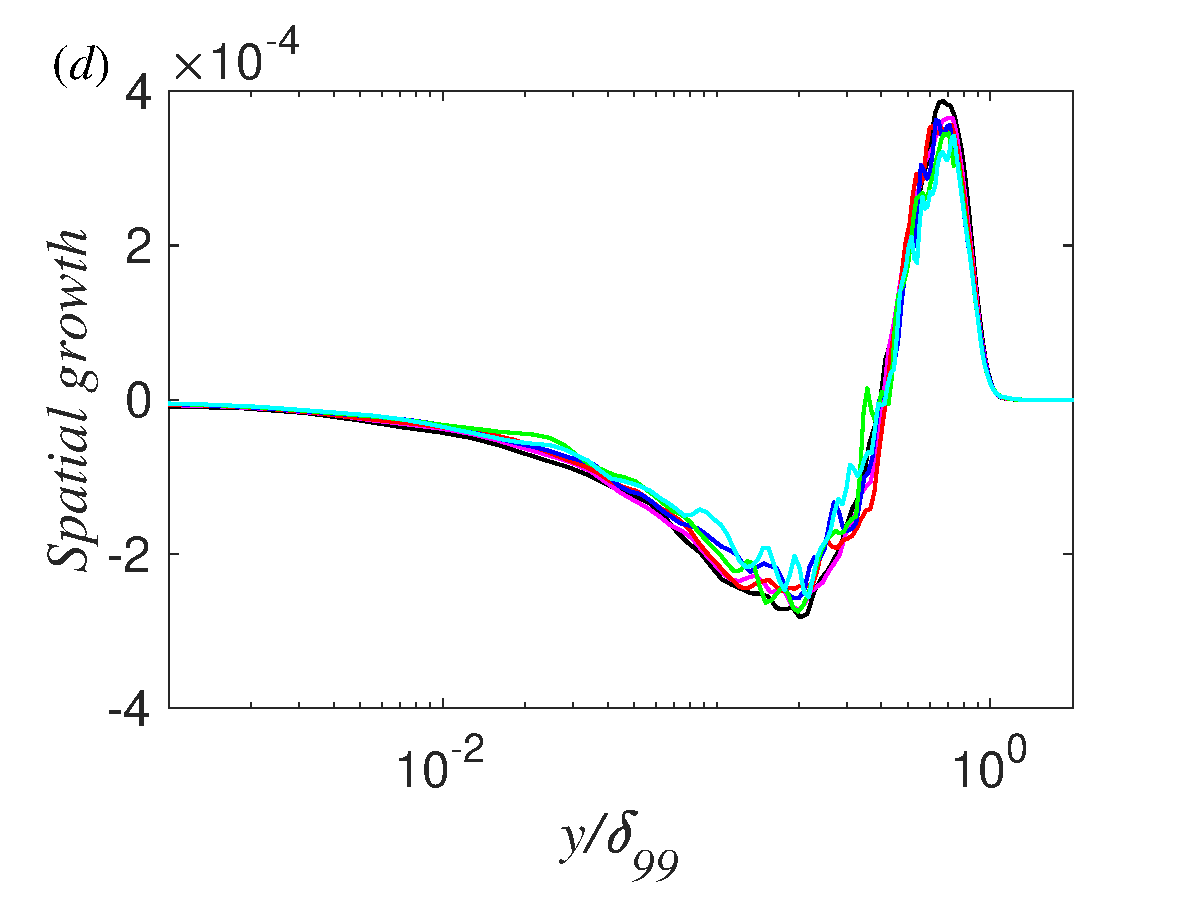
\includegraphics[width = 6cm]{7d}\label{balan:d}}
\caption{{\color{black}Distributions of the ($y/\delta_{99}-$)pre-multiplied power of viscous and turbulent stress ($a$), viscous dissipation ($b$), turbulence kinetic energy production ($c$), and spatial growth ($d$) for the APG-TBL with $\beta\approx1.4$.}}
\label{balan}
\end{figure}



}


\subsection{Mean friction drag decomposition of the APG-TBLs on NACA4412 wing section}

For the APG-TBLs on the suction side of the NACA4412 wing section at $Re_c=200,000$, 400,000, and 1,000,000, the pressure-gradient parameters ($\beta$) are much higher than those  on the flat plates.  Figure \ref{evolution:a} shows the distributions of $\beta$  along the suction side of various cases, focusing on the range of $0.4<x/c<0.95$. Note that near the leading edge of the airfoil ($x/c<0.4$), the magnitude of the APG is limited within $\beta \lesssim 1$, and under the very strong APG conditions observed for $x/c>0.95$,  it may be inappropriate to use $\beta$ to characterize the effects of pressure gradients on TBLs~\cite{Vinuesa2018,Kitsios2017}.




Figure \ref{evolution:b} shows the streamwise evolution of the contributing components ($C_{f1}/C_f$, $C_{f2}/C_f$, and $C_{f3}/C_f$) for the three Reynolds numbers. The relative errors  $[(C_{f1}+C_{f2}+C_{f3})-C_f]/C_f$ are within $\pm0.96\%$, which indicates that the RD identity is also reliable when analyzing the mean friction drag on the airfoils. 
Similar trends are observed for the various components at the three values of $Re_c$.  The magnitude of $C_{f1}/C_f$ is much smaller than the other two components, especially near the trailing edge of the airfoil, where $\beta$ becomes very large. 
Regardless of $Re_c$, the positive $C_{f2}/C_f$ increases, and the negative $C_{f3}/C_f$ decreases for increasing $x$.
At the same position on the airfoil,  larger $Re_c$ leads to relatively smaller positive contribution of $C_{f2}$ and negative contribution of $C_{f3}$. Note that these observations correspond to the NACA4412 wing section, but they do not necessarily apply to other airfoils.

The effect of Reynolds number for a fixed value of $\beta$ on the suction-side APG-TBL is evaluated next. To this end, in figure \ref{ret_beta} we show the distributions of $\beta$ as a function of $Re_\tau$ for the three wings. 
We will consider the values $\beta=2$, 4, and 8, marked with circles, squares and triangles, respectively in figure \ref{ret_beta}, in our analysis.  

Figure \ref{naca} quantifies the wall-normal distributions of the pre-multiplied integrands in $C_{f1}/C_f$, $C_{f2}/C_f$, and $C_{f3}/C_f$ at $\beta \approx2$, 4, and 8. 
It can be seen that regardless of the pressure-gradient coefficient and the Reynolds number, (i) the inner peaks of the $C_{f1}$- and $C_{f2}$-contributions are fixed at $y^+\approx6$ and $y^+\approx16.5$, respectively; (ii) the positions of the outer peaks in the $C_{f1}$- and $C_{f2}$-contributions are well-scaled by the outer scale at $y/\delta_{99}\approx0.7$ and $y/\delta_{99}\approx0.53$, respectively; and (iii) the valleys and peaks of the
$C_{f3}$-contributions scale well in outer units, and they are located  at $y/\delta_{99}\approx0.1$ and $y/\delta_{99}\approx0.65$, respectively. These features are the same as the observations in APG-TBLs on flat plates with constant $\beta$. 

With the same $\beta$, the effects of the Reynolds number on the peak values are more evident in the APG-TBLs on the NACA4412 airfoil: 
(i) both the inner- and outer-peak values of the $C_{f1}$- and $C_{f2}$-contributions decrease as $Re_\tau$ increases, confirming the finding~\cite{Vinuesa2018} that the higher-$Re$ TBLs are less sensitive to APG effects;
(ii) both the valleys and peaks of the $C_{f3}$-contributions attenuate with the increase of Reynolds number, due to the reduced contributions of the convection and pressure gradient to the skin-friction drag generation (not shown here).


%Note that all of the three cases are subjected to approximately the same distribution of $\beta(x_a)$, thus their differences could be deemed to be ascribed to the Reynolds-number effects only.


\begin{figure}
\subfigure{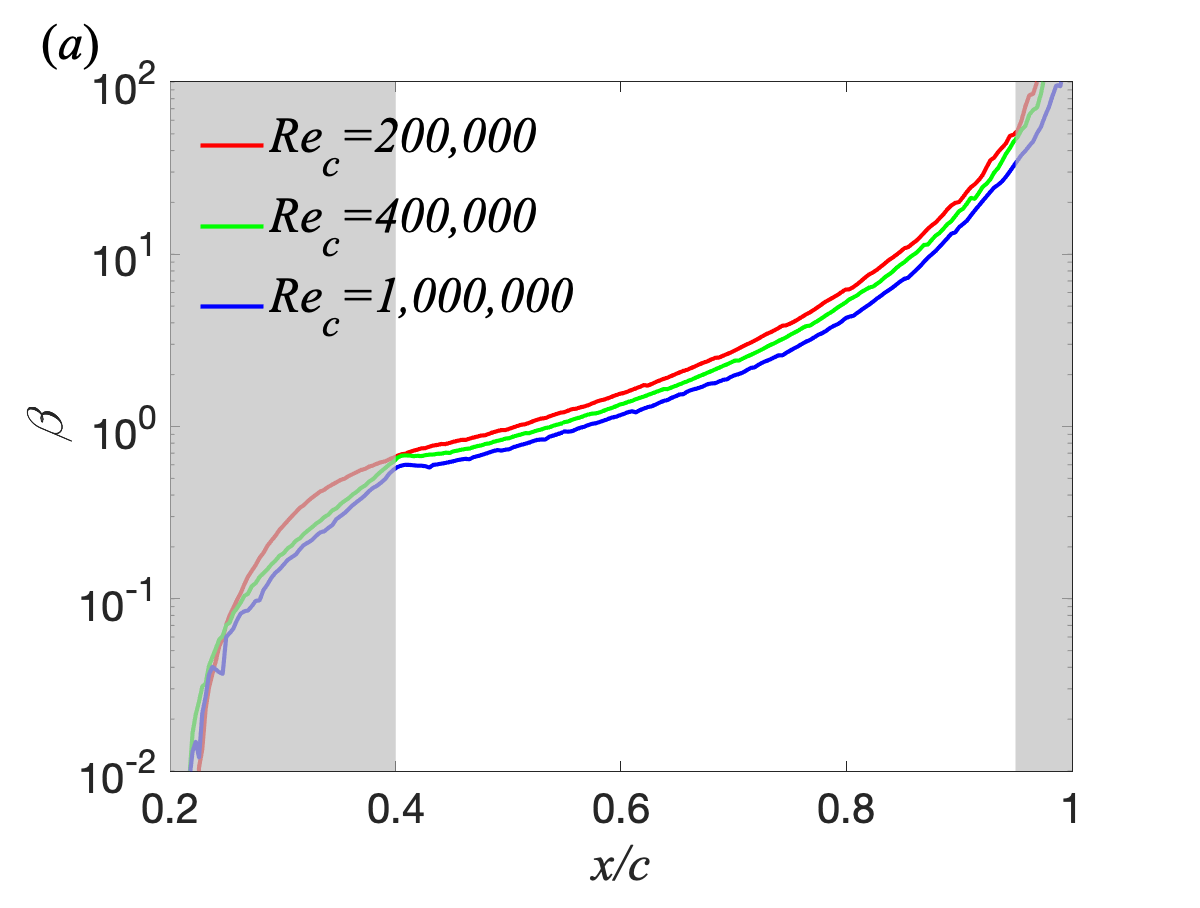
\includegraphics[width = 6cm]{8a}\label{evolution:a}}
\subfigure{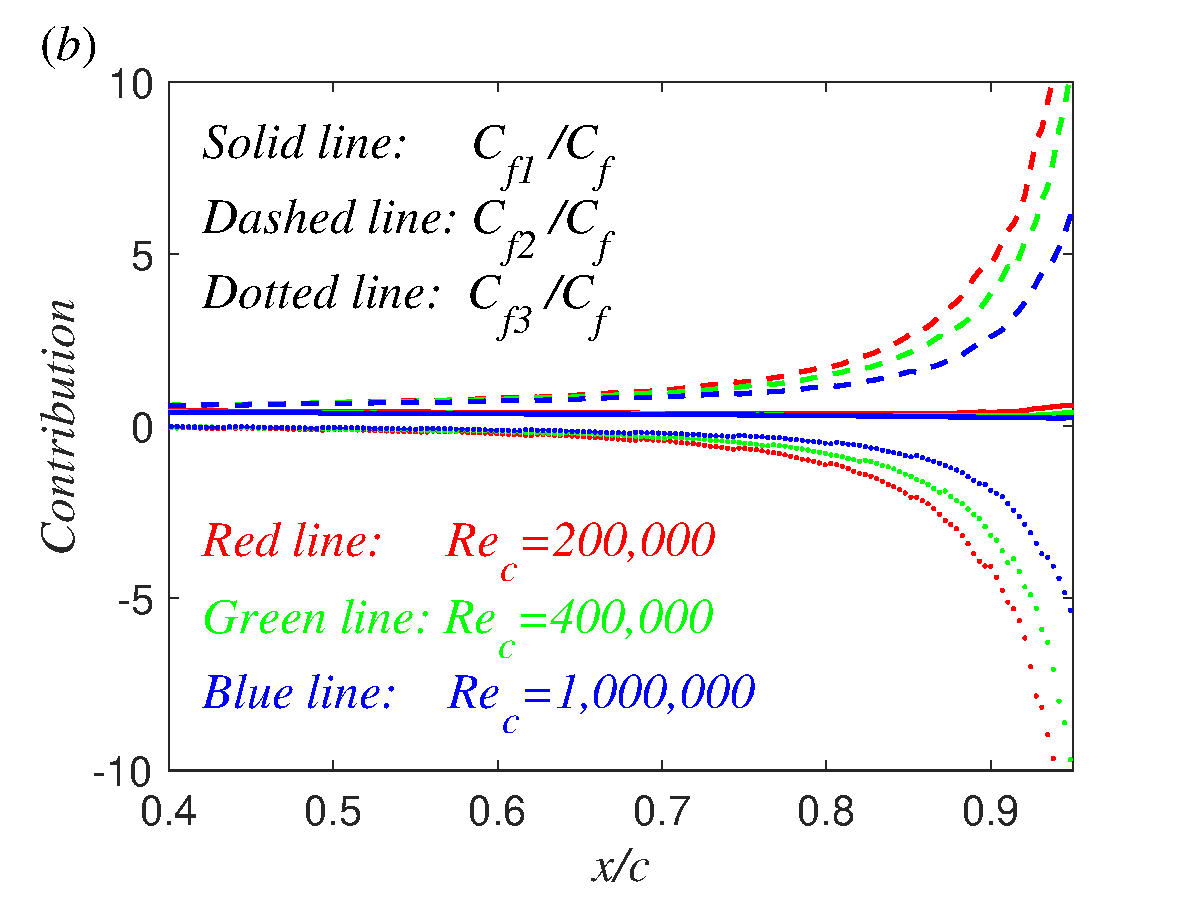
\includegraphics[width = 6cm]{8b}\label{evolution:b}}
\caption{($a$) Distribution of $\beta$ as a function of $x/c$ on the suction side of the NACA4412 wing section for the three Reynolds numbers. The shaded areas are excluded from this study. ($b$) The ratio of each contribution to the total friction coefficient for the airfoil APG-TBLs.}
\label{evolution}
\end{figure}

\begin{figure}[h]
\centering
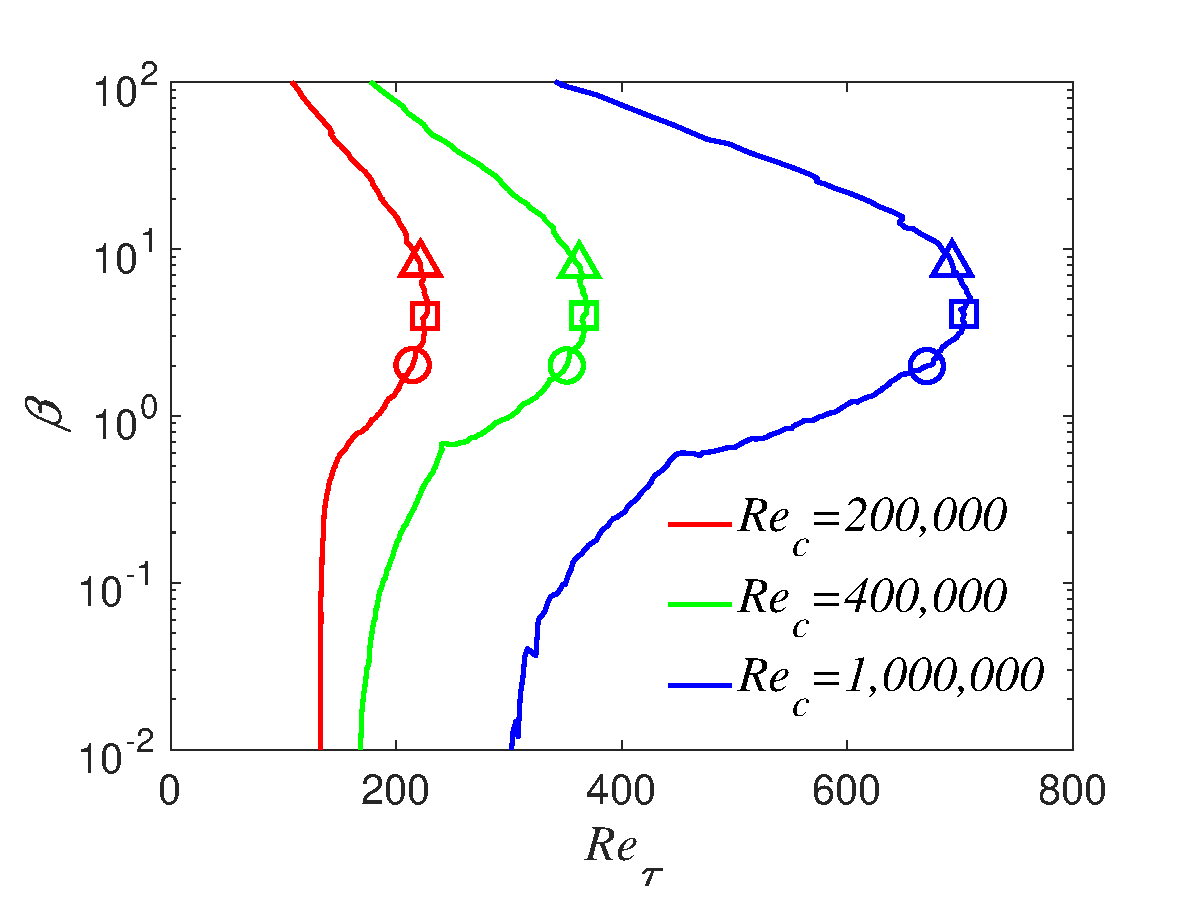
\includegraphics[width = 8cm]{9}
\caption{Distributions of $\beta$ as a function of $Re_\tau$ on the suction side of the NACA4412 airfoil. The three values of $\beta$, i.e. $\beta=2$, 4 and 8, are represented by a circle, a square, and a triangle, respectively.}
\label{ret_beta}
\end{figure}


\begin{figure}[h]
% \subfigure{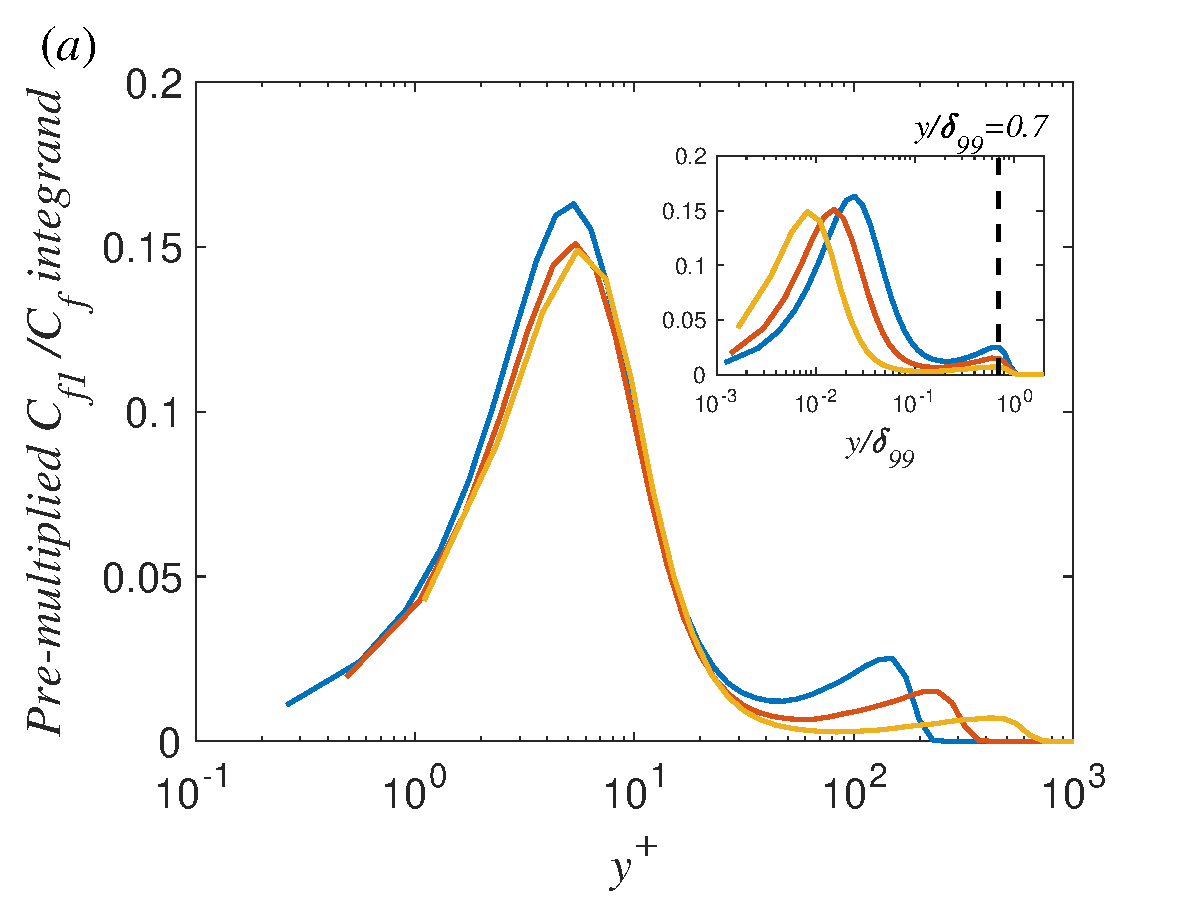
\includegraphics[width = 4cm]{10a}\label{naca:a}}
% \subfigure{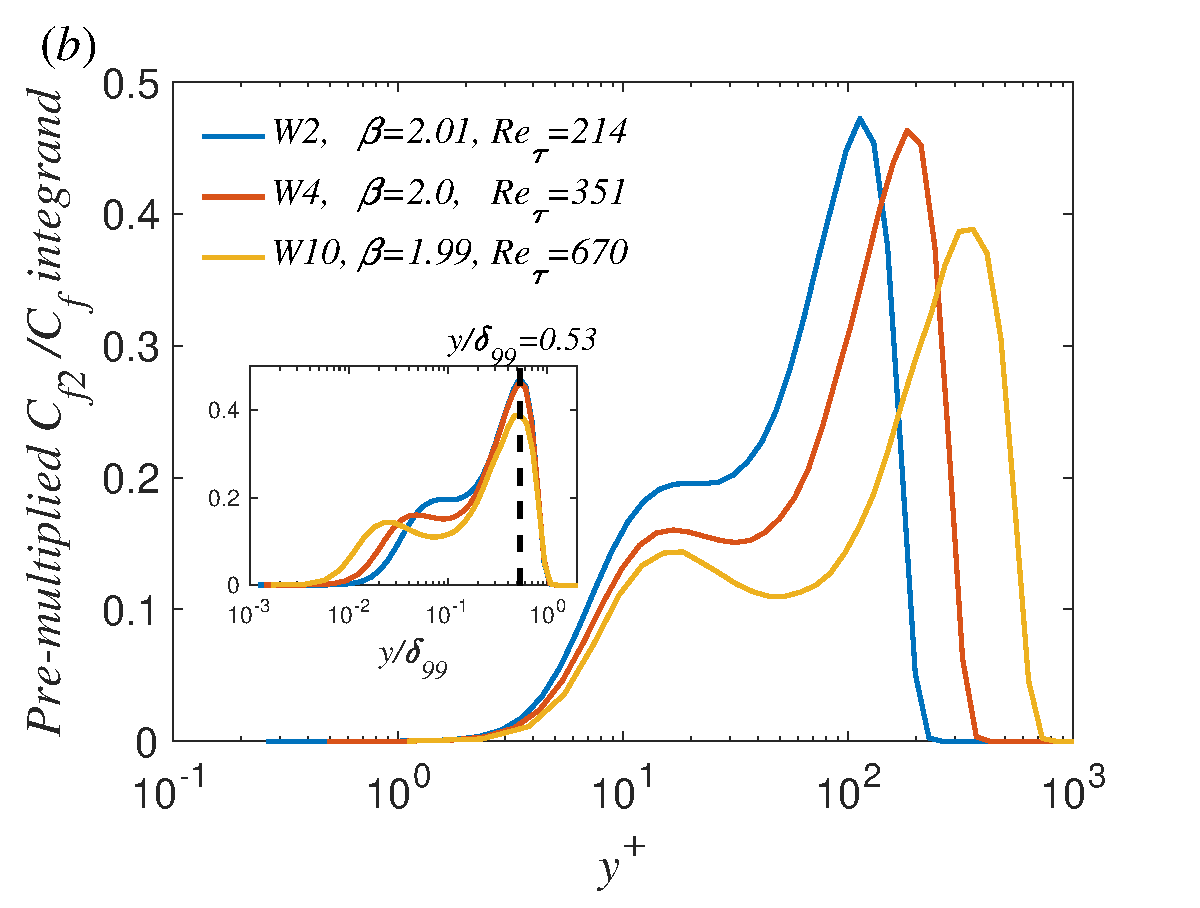
\includegraphics[width = 4cm]{10b}\label{naca:b}}
% \subfigure{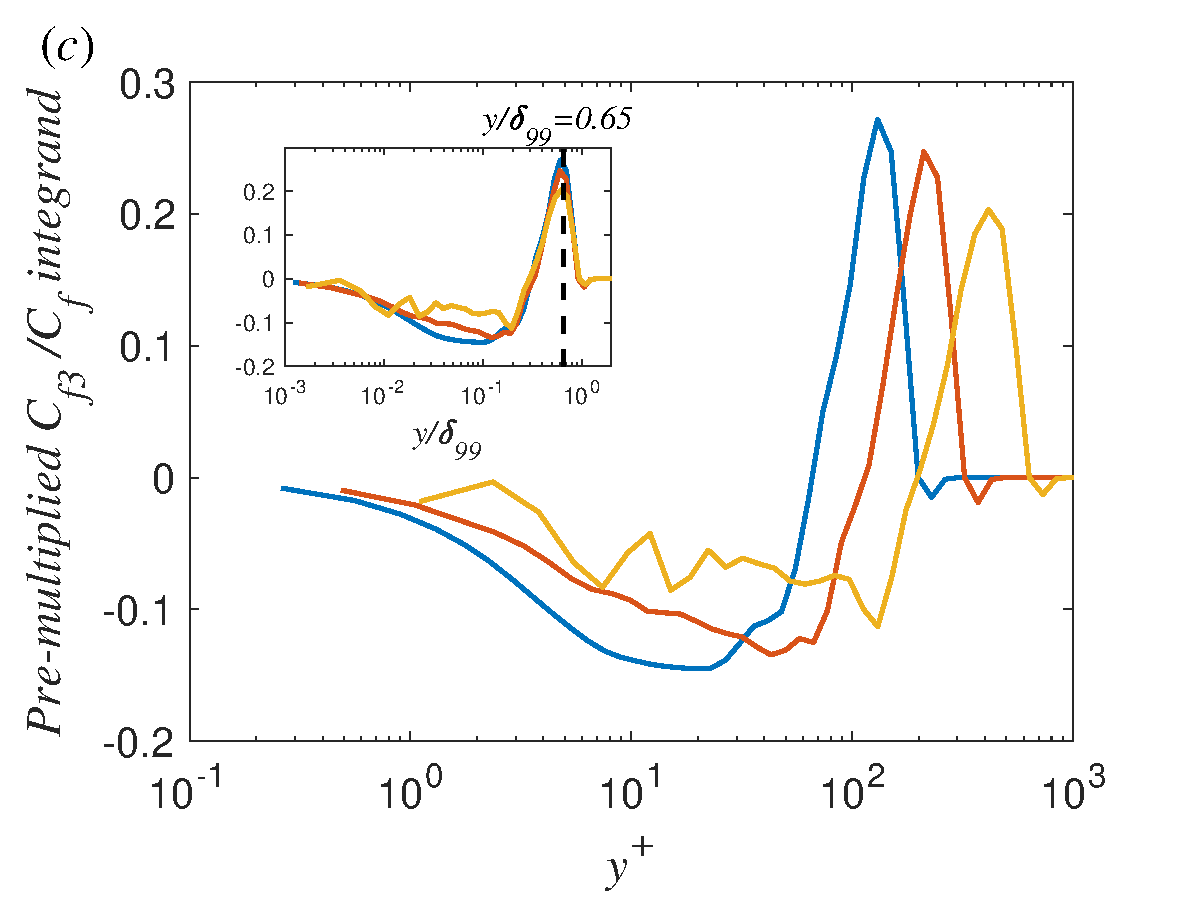
\includegraphics[width = 4cm]{10c}\label{naca:c}}
% \subfigure{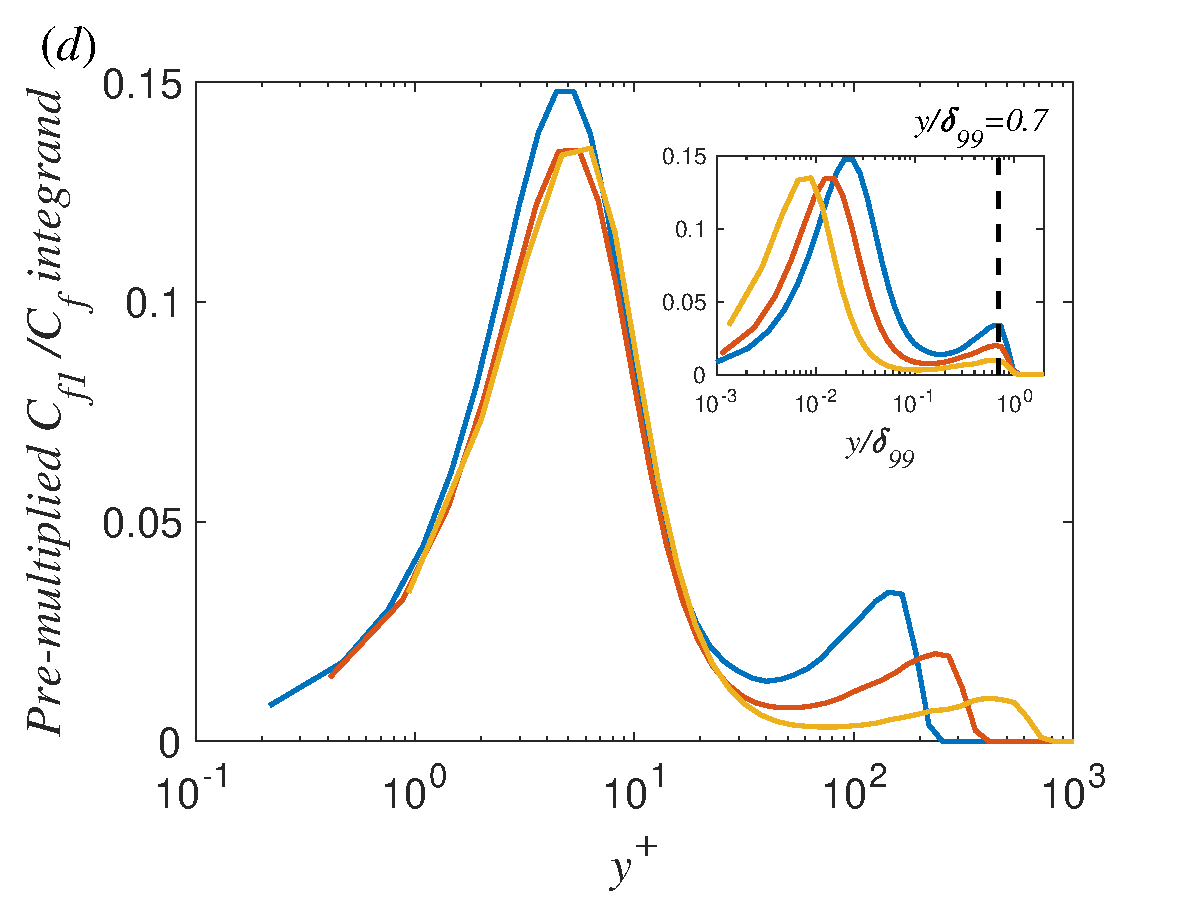
\includegraphics[width = 4cm]{10d}\label{naca:d}}
% \subfigure{\includegraphics[width = 4cm]{10e}\label{naca:e}}
% \subfigure{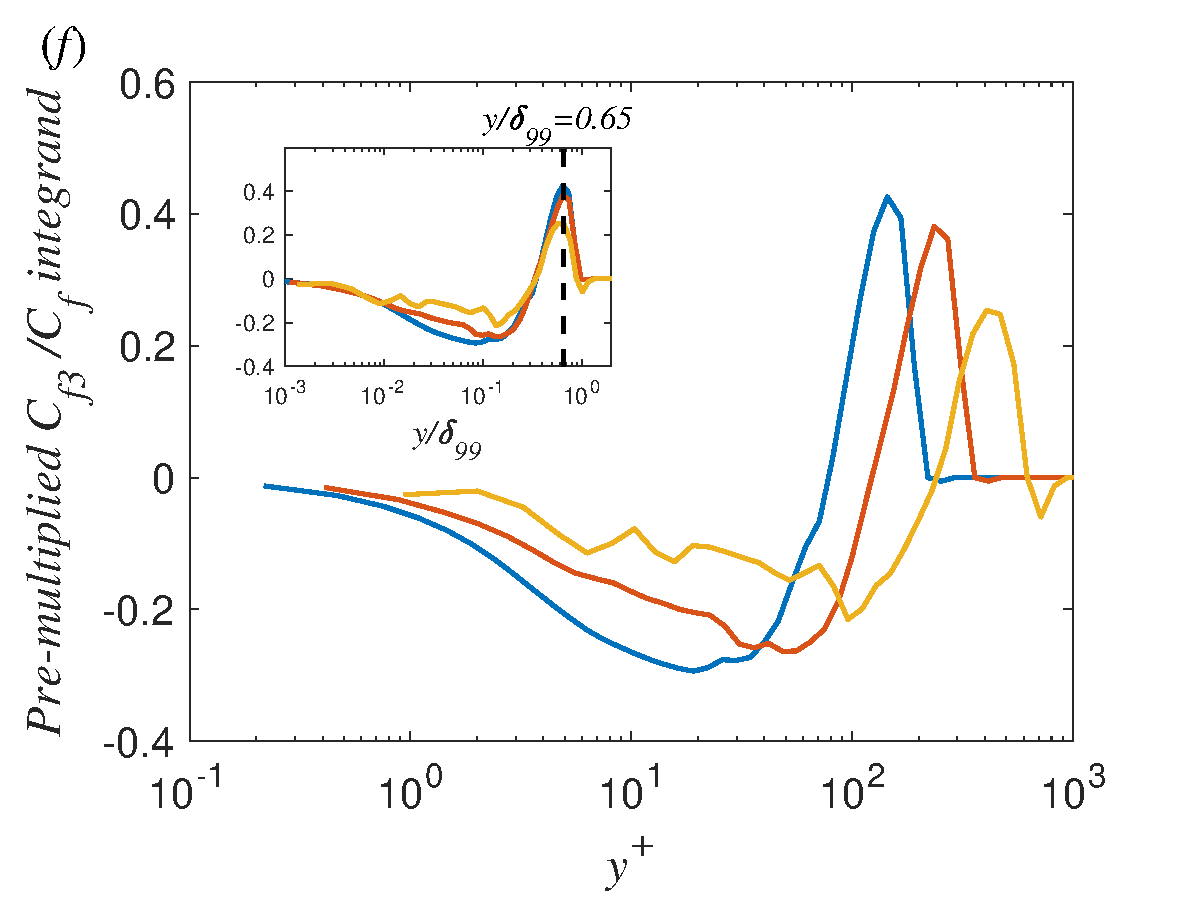
\includegraphics[width = 4cm]{10f}\label{naca:f}}
% \subfigure{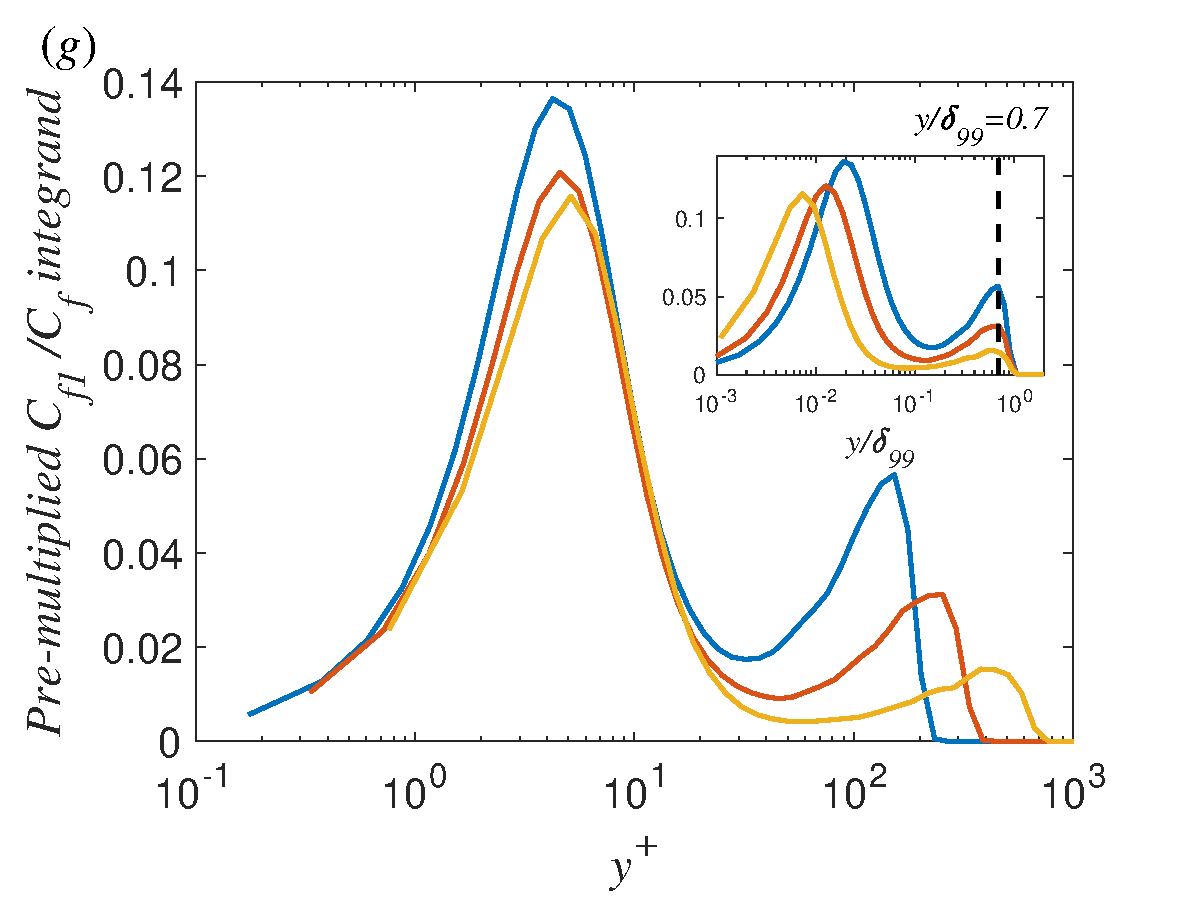
\includegraphics[width = 4cm]{10g}\label{naca:g}}
% \subfigure{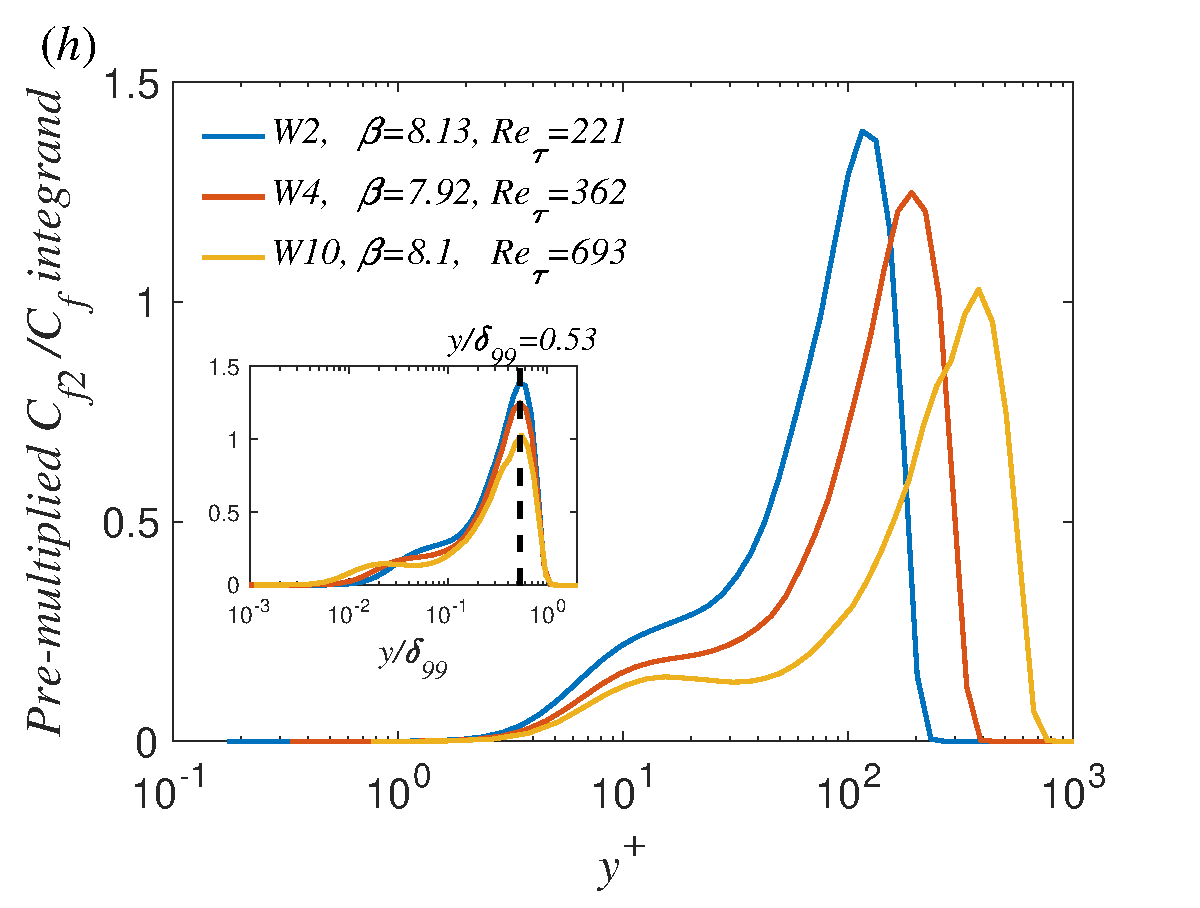
\includegraphics[width = 4cm]{10h}\label{naca:h}}
% \subfigure{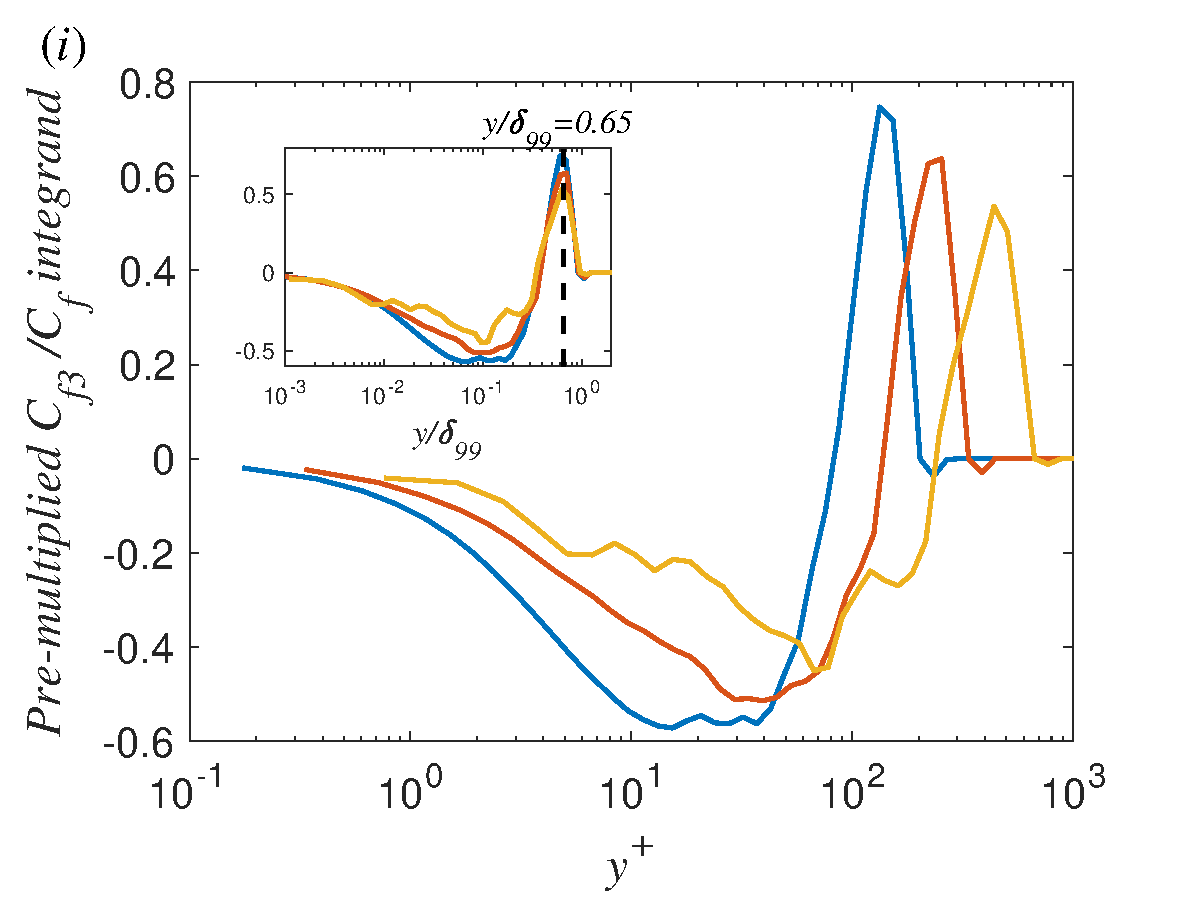
\includegraphics[width = 4cm]{10i}\label{naca:i}}
{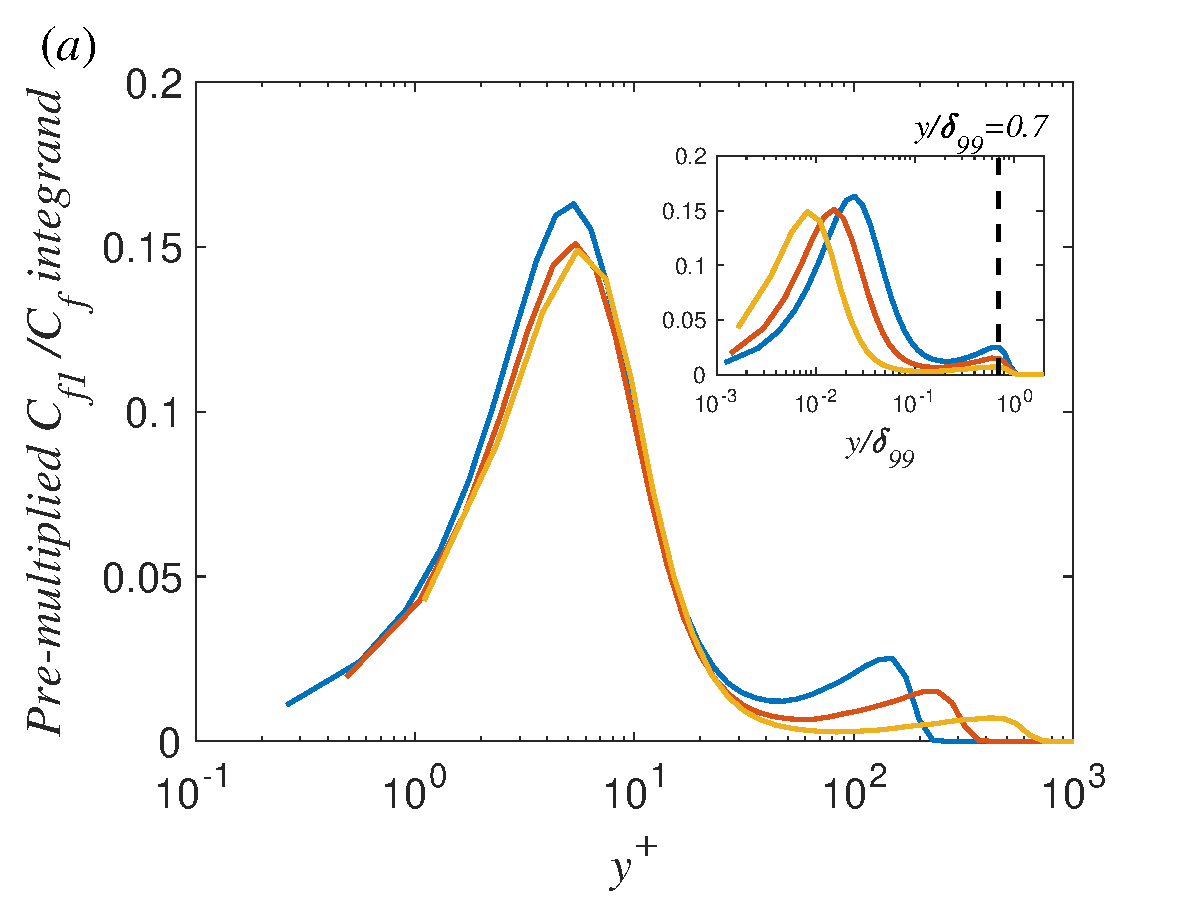
\includegraphics[width = 3.8cm]{10a}\label{naca:a}}
{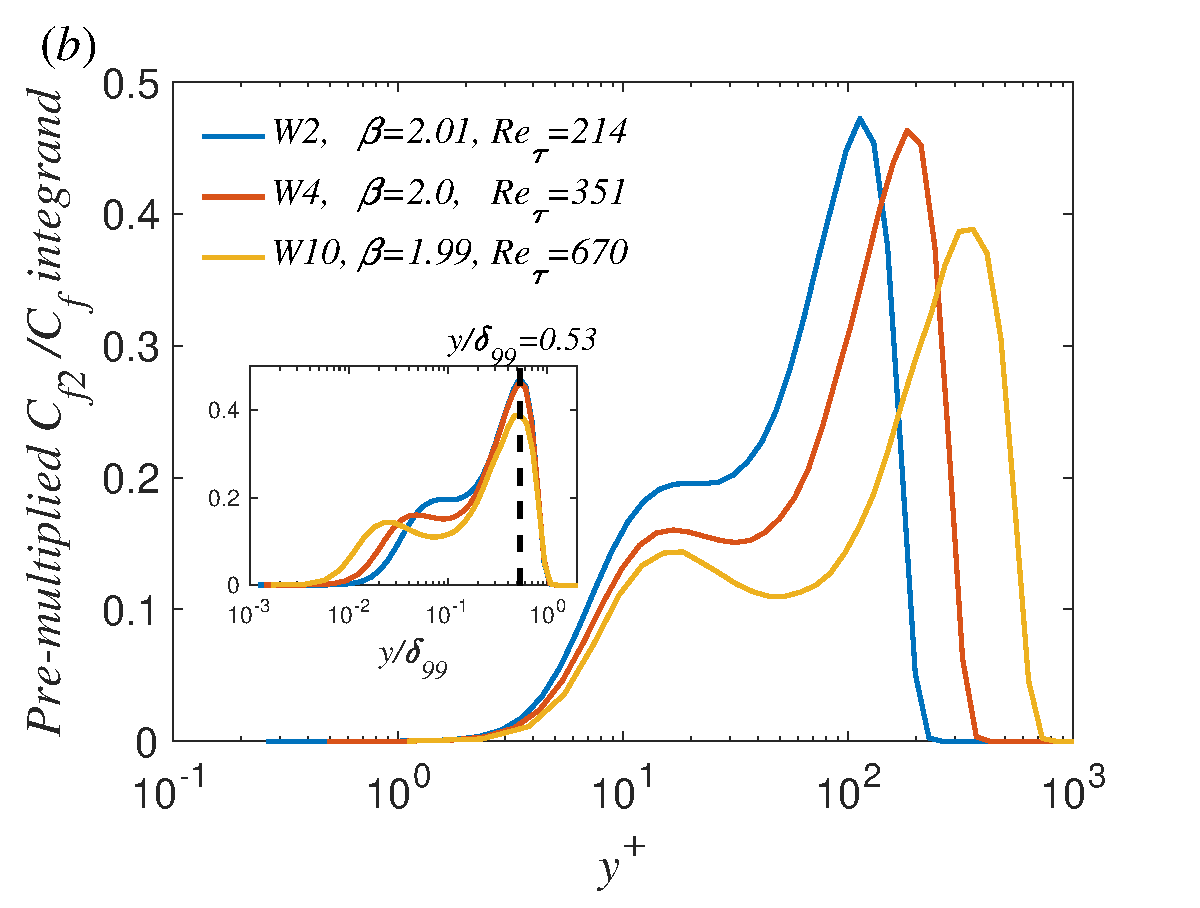
\includegraphics[width = 3.8cm]{10b}\label{naca:b}}
{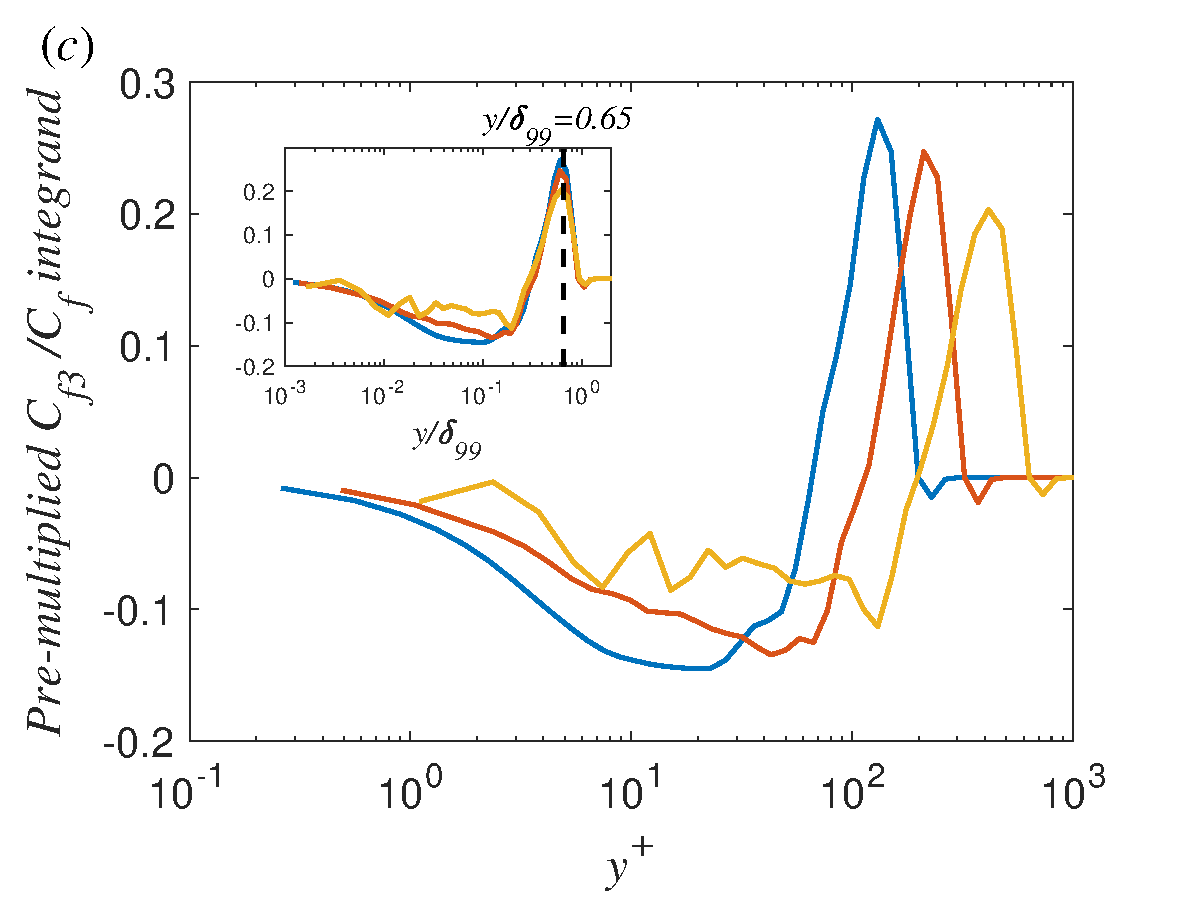
\includegraphics[width = 3.8cm]{10c}\label{naca:c}} \\
{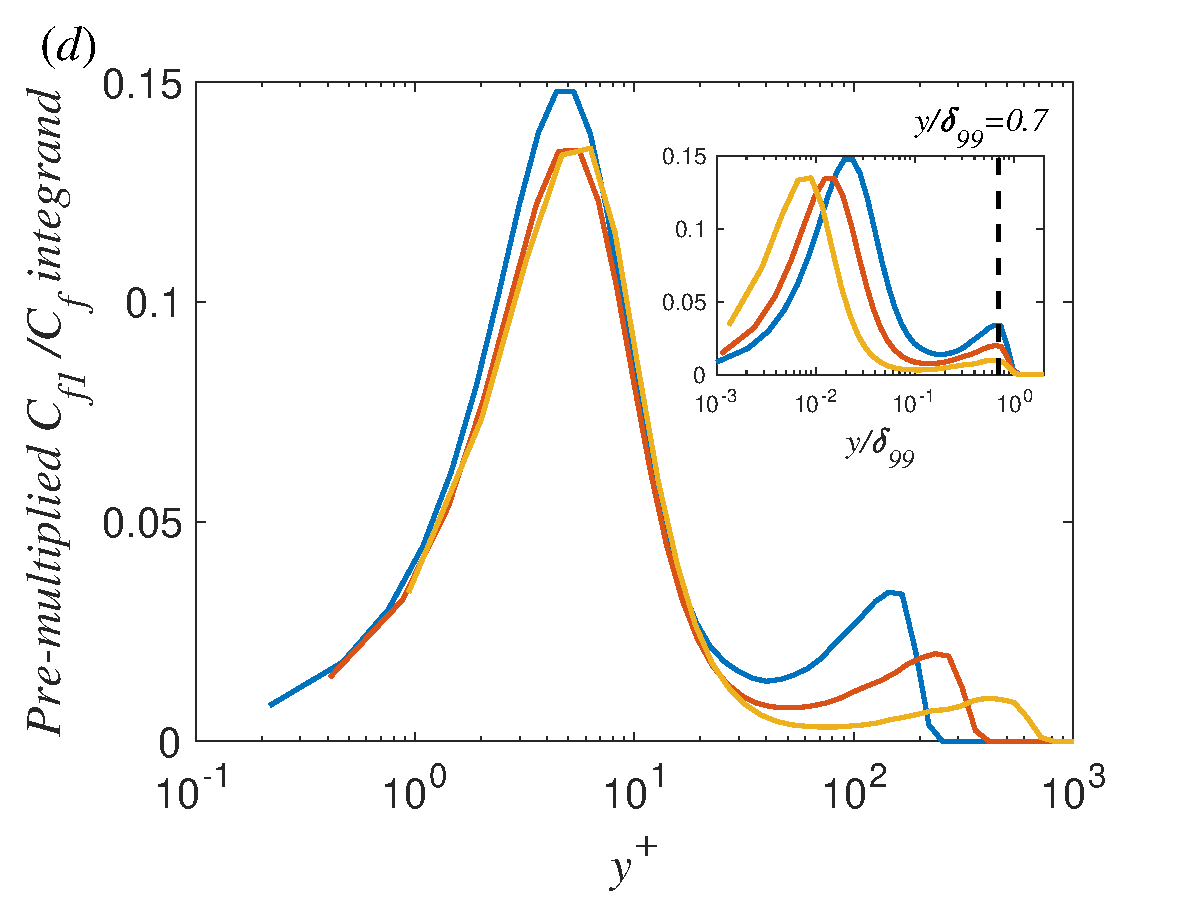
\includegraphics[width = 3.8cm]{10d}\label{naca:d}}
{\includegraphics[width = 3.8cm]{10e}\label{naca:e}}  
{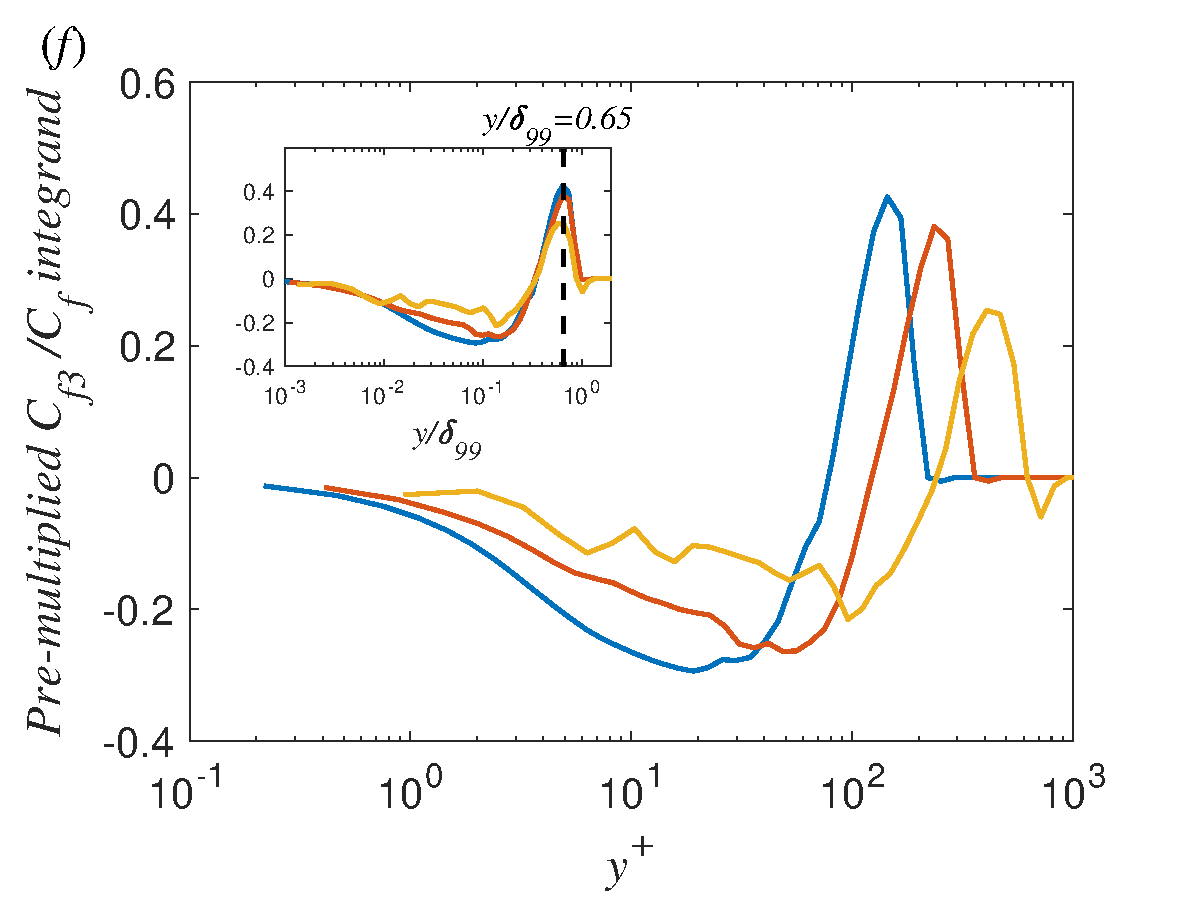
\includegraphics[width = 3.8cm]{10f}\label{naca:f}} \\
{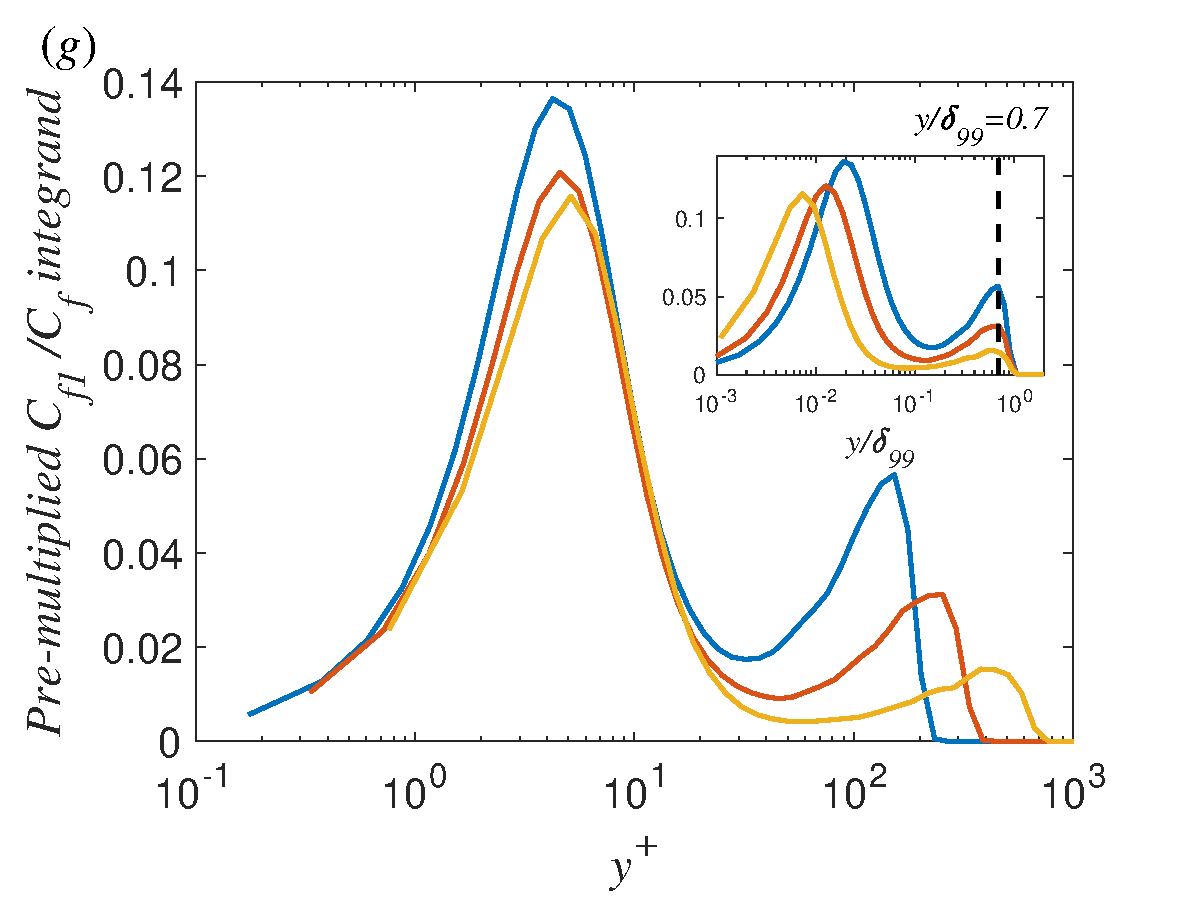
\includegraphics[width = 3.8cm]{10g}\label{naca:g}}
{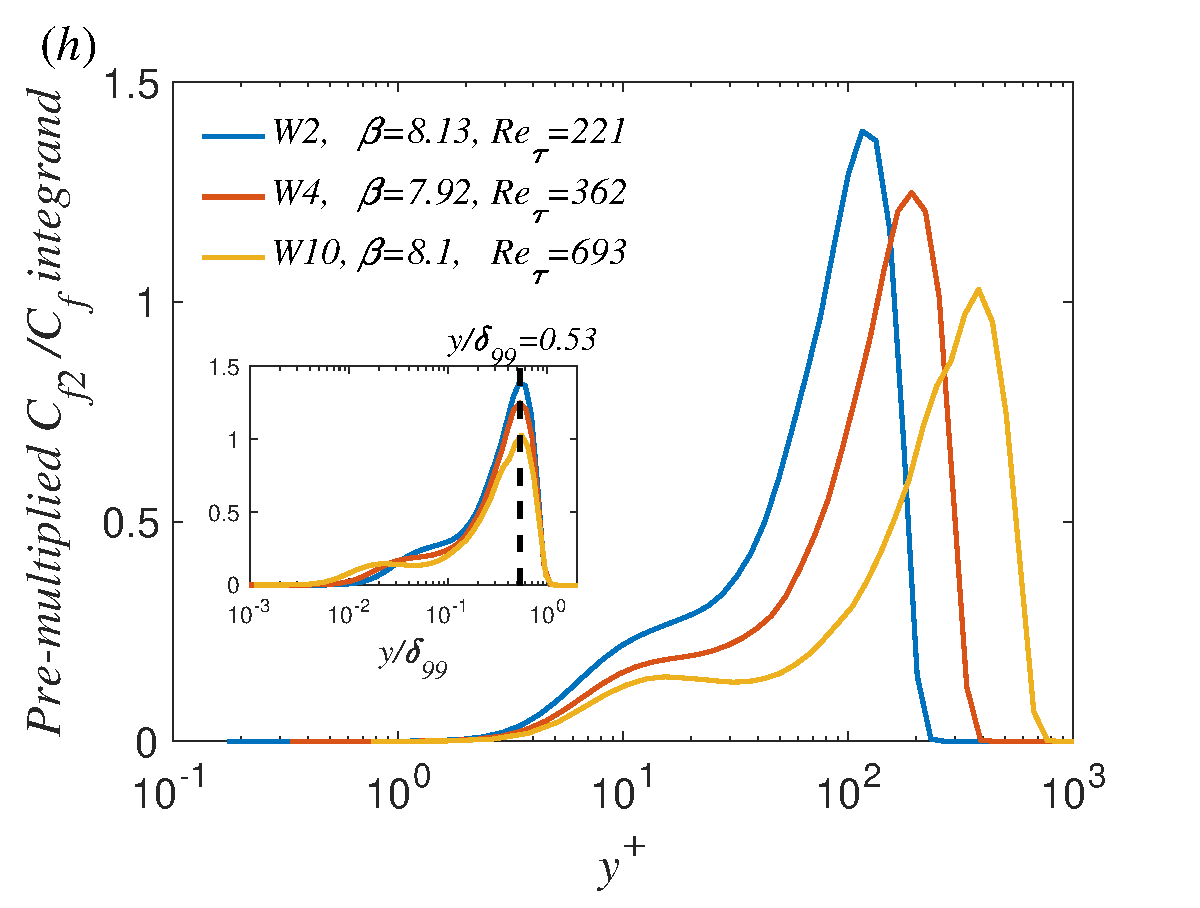
\includegraphics[width = 3.8cm]{10h}\label{naca:h}}
{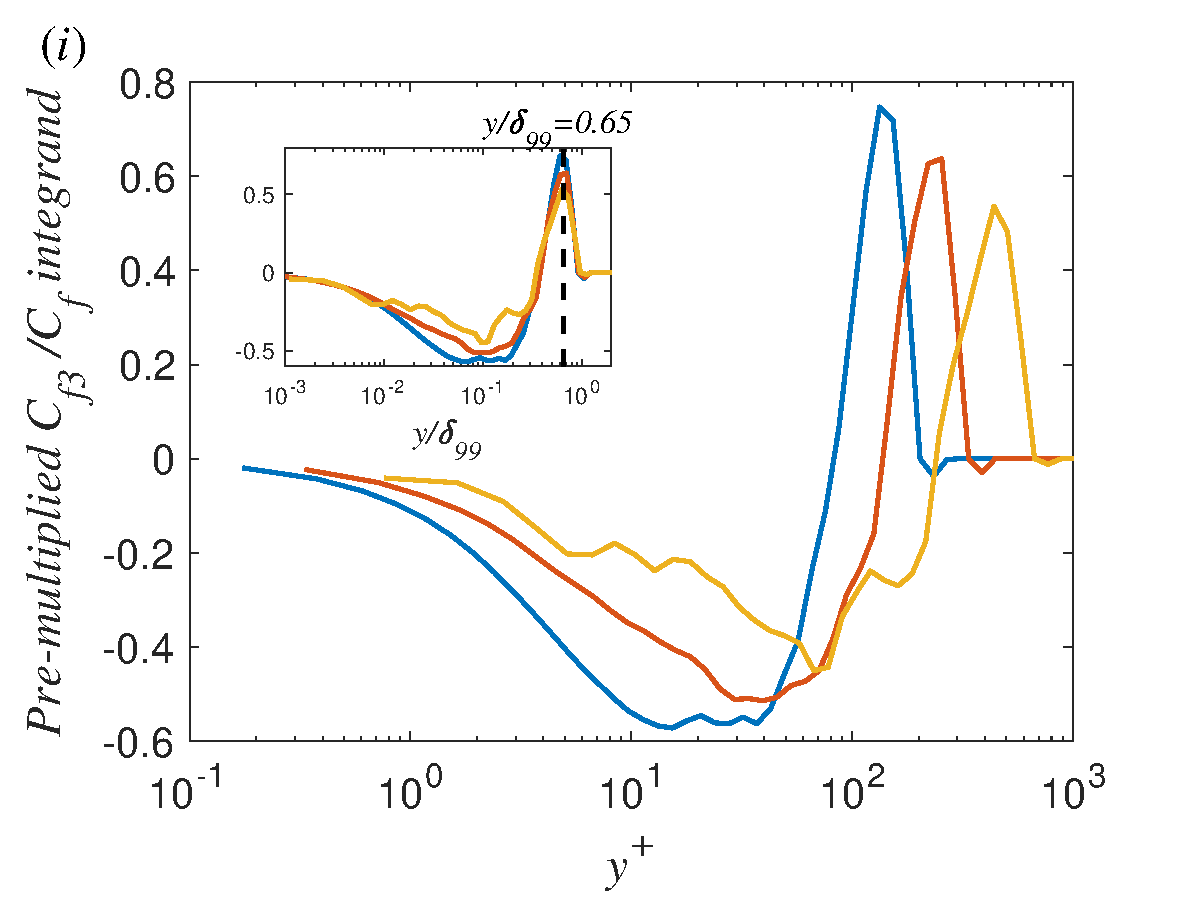
\includegraphics[width = 3.8cm]{10i}\label{naca:i}}
\caption{Distributions of the pre-multiplied integrand in $C_{f1}/C_f$ ($a, d, g$) , $C_{f2}/C_f$ ($b, e, h$), and $C_{f3}/C_f$ ($c, f, i$) as a function of $y^+$ for the airfoil APG-TBLs at three different $\beta$. Top, middle, and bottom rows correspond to the conditions denoted by circle, square, and triangular in figure \ref{ret_beta}, respectively,}
\label{naca}
\end{figure}



%The existence of adverse pressure gradient introduces a strong driving force into the turbulent boundary layers, leading to the negative component $C_{f3}$.
%A different result is found in the variation of $C_{f2}/C_f$ with regard to the Reynolds number at high pressure-gradient parameters in figure \ref{dec_naca}. Especially when $x_a>0.7$, $C_{f2}/C_f$ decreases with the increase of $Re_\tau$ under the condition of the same $\beta$ and similar $\beta$-history (i.e. at a specific location of $x_a$), which is contradictory to the result in ZPG-TBLs. It again suggests that the TBLs with higher-Re is less sensitive to APG effects, which thus has less contribution to $C_{f2}$.
%As stated by \citet{Vinuesa2018}, cases of NACA4412 at $Re_c=200,000$, 400,000 and 1,000,000 have very similar distributions of $\beta(x_a)$. Thus their differences in flow properties could be attributed to the Reynolds-number effects. 
%
%Whereas the locations of the secondary peaks are well-scaled in outer units, and fixed at $y/\delta_{99}\approx0.7$ and $y/\delta_{99}\approx0.53$ in $C_{f1}$- and $C_{f2}$-contributions respectively, with their values decreasing with the Reynolds number, re-confirming the finding that the higher-$Re$ TBLs are less sensitive to APG effects.
%In addition, as $\beta$ increases, both the outer-layer contribution of $C_{f1}$ and $C_{f2}$ to the skin friction dramatically increases, e.g. the outer-peak value of $C_{f1}$-contribution achieves nearly half of the inner peak at $\beta=8.13$ and $Re_\tau=221$.
%%This is in good agreement with the previous finding that the dominant secondary peak of production is approximately located at the half height of the boundary layer thickness \cite{Skare1994}.
%
%At last, as depicted in figures \ref{naca:g}-\ref{naca:i}, both the valley and peak of the pre-multiplied $C_{f3}/C_f$ integrand are more collapsed in outer units, i.e. $y/\delta_{99}\approx0.1-0.2$ and $y/\delta_{99}\approx0.65$, respectively, in accordance with the statements in Sec.~\ref{Re-eff}. 
%
%At higher Reynolds numbers, the smaller valley and peak values manifest reduced contributions of the convection and pressure gradient to the skin-friction drag generation.




\subsection{Pressure-gradient-history effects on the mean friction drag decomposition}\label{hist}

The $\beta$-history effect on the mean friction decomposition is also considered in this paper. 
As reported in \citet{Bobke2017} and \citet{Tanarro2020}, besides $\beta$ and $Re_\tau$, the history of $\beta$ is also an important parameter to characterize the state of the APG-TBLs. 
Figure \ref{cross} shows the $\beta-Re_\tau$ diagram by using the cases of $\beta1$, $\beta2$, $m18$, $W4$ and $W10$. 
Three different conditions with the same $\beta$ and $Re_\tau$ but different $\beta$-histories  are selected from  figure \ref{cross} and marked with a triangular ($P_1$), a circle ($P_2$), and a star ($P_3$). 
At $P_1$,  the variation of $\beta$ exhibits an increasing trend but with different slopes in the two cases; $P_2$ involves two cases with an increasing and decreasing trend, respectively; and at $P_3$, the approximately invariant $\beta(Re_\tau)$ intersects the increasing $\beta$ trend from the wing case. 
Similar results can be found for other intersections in figure \ref{cross}, but are not shown here for brevity. 

\begin{figure}[htb]
\centering
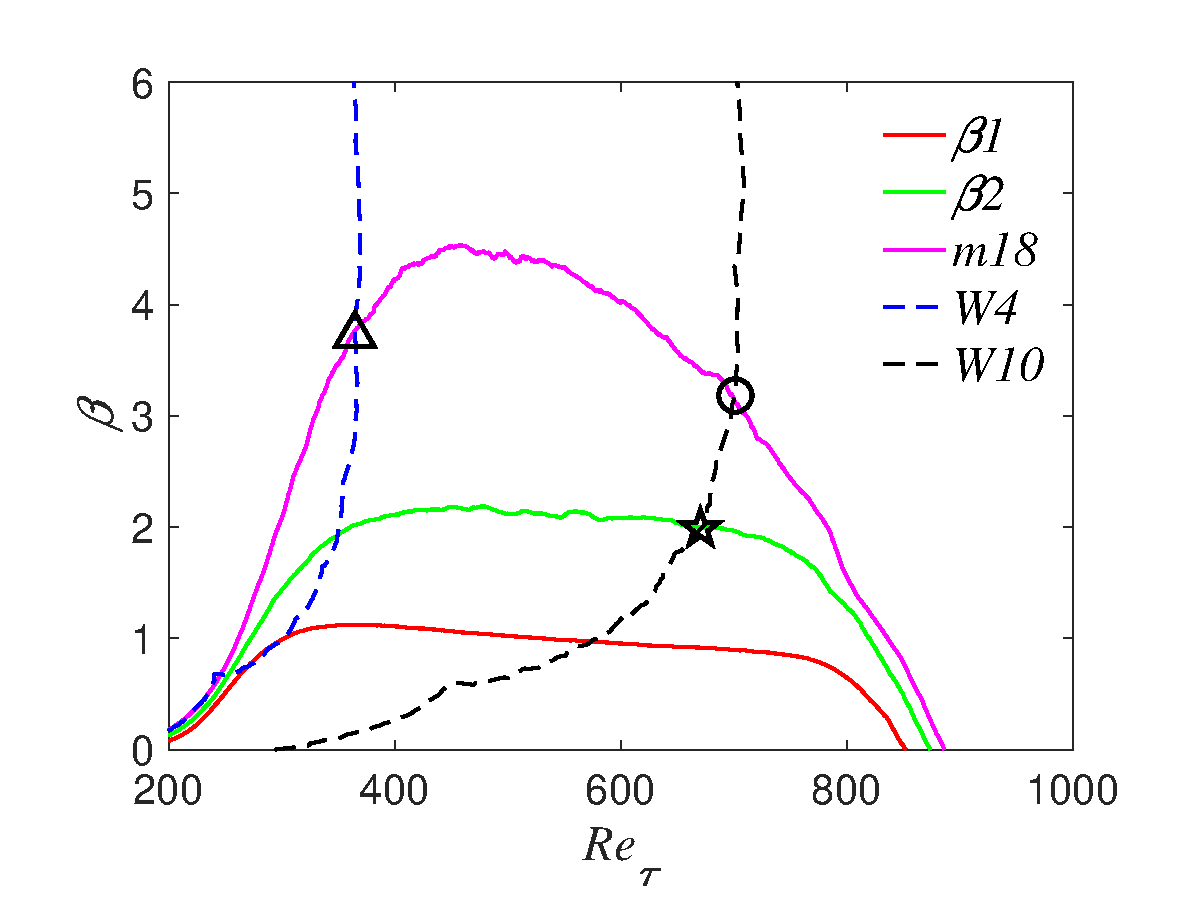
\includegraphics[width = 8cm]{11}
\caption{Distribution of the pressure-gradient parameter $\beta$ as a function of the friction Reynolds number $Re_\tau$ for various APG-TBL cases. The conditions $P_1$, $P_2$ and $P_3$ are denoted by a triangle, a circle and a star, respectively. }
\label{cross}
\end{figure}

\begin{table}
\begin{center}
  \fontsize{8.0pt}{10.25pt}\selectfont
  \addtolength{\tabcolsep}{-2pt}
\def~{\hphantom{0}}
\caption{Skin-friction drag coefficients of APG-TBLs with different histories of $\beta$, for the conditions shown in figure \ref{cross}.}\label{tab:2} 
\begin{tabular}{|c|c|c|c|c|c|c|}
	\hline
    \multirow{2}{*}{Case} 
    & \multicolumn{2}{c|}{$P_1$}    &   \multicolumn{2}{c|}{$P_2$} &   \multicolumn{2}{c|}{$P_3$} \\
    \cline{2-7}
     & $m18$	&	$W4$ &	$m18$   &	 $W10$    &   $\beta$2   &   $W10$ 	\\
	\hline
	$C_f$ & $2.2\times10^{-3}$	&	$2.6\times10^{-3}$ &		$1.7\times10^{-3}$   &	 $2.3\times10^{-3}$    &   $2.2\times10^{-3}$   &   $2.6\times10^{-3}$\\
	\hline
\end{tabular}
\end{center}
\end{table}

Table~\ref{tab:2} gives the mean friction drag coefficients of the APG-TBLs at points $P_1$--$P_3$, which exhibit different histories of $\beta$. It can be noted that the development history of $\beta$ has an impact on the local skin-friction coefficient, and stronger accumulated $\beta$ values lead to lower $C_f$.
Figure \ref{history} shows the wall-normal distributions of the pre-multiplied integrands for cases $P_1$--$P_3$. Both the inner and outer peaks of the three friction terms are located at the same $y^+$, which is unaffected by the $\beta$-history. 
However, several redistributions of the friction contributions along the wall-normal direction can be observed. For the APG-TBLs with a higher upstream-$\beta$, i.e. $m18$ at $P_1$, $m18$ at $P_2$, and $\beta$2 at $P_3$, larger contributions to $C_{f1}/C_f$, $C_{f2}/C_f$ and $C_{f3}/C_f$ are observed in the outer region, associated with the enhancement of both small- and large-scale activities in the outer region, whereas the role of inner-layer dynamics is decreased in the contribution of $C_{f1}$ and $C_{f2}$.
%As for the cases at $P_2$, such phenomena are not much evident due to the very close development of $\beta$.
This implies that the upstream development of the pressure gradient can be accumulated and the higher upstream-$\beta$ leads to a more pronounced outer-layer contribution to skin-friction drag whereas it reduces the significance of inner-layer dynamics.



\begin{figure}[htb]
\subfigure{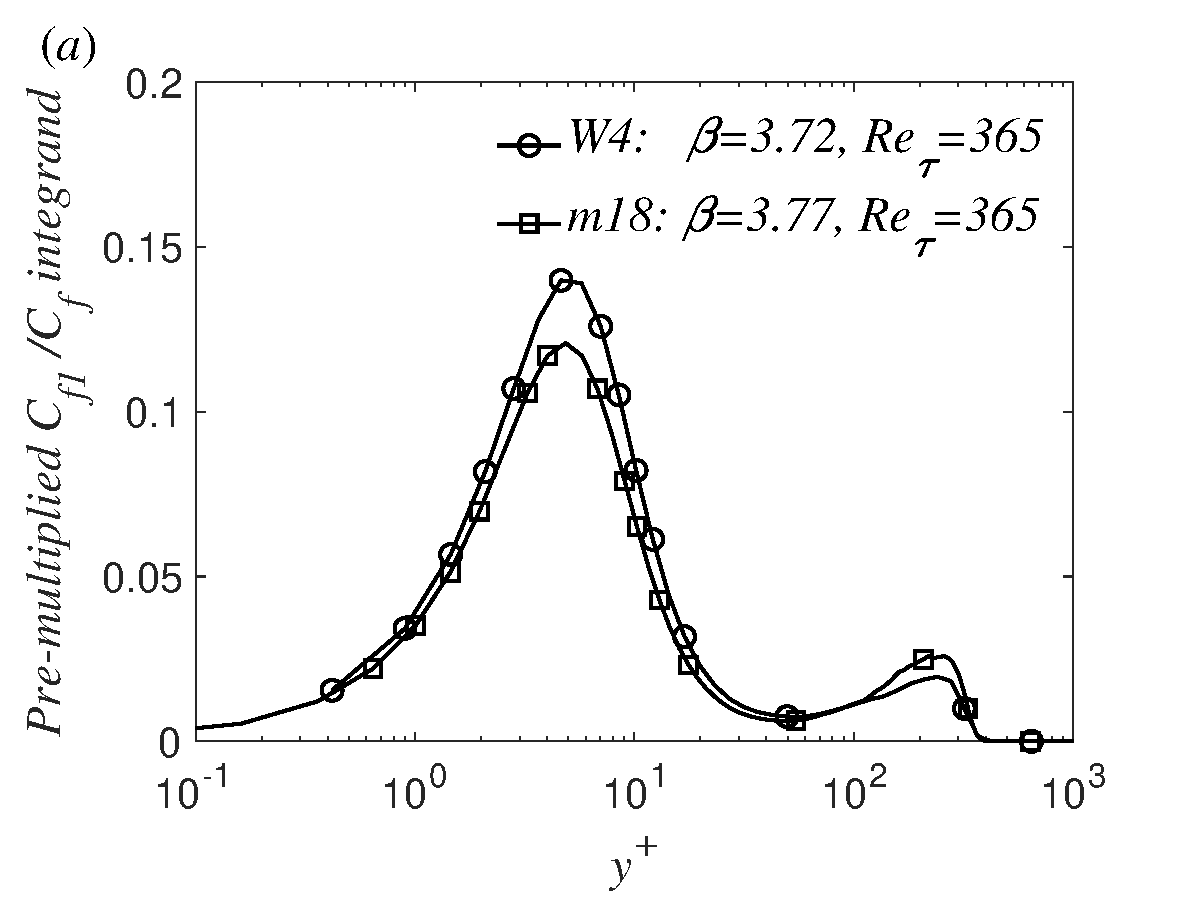
\includegraphics[width = 5cm]{12a}}
\subfigure{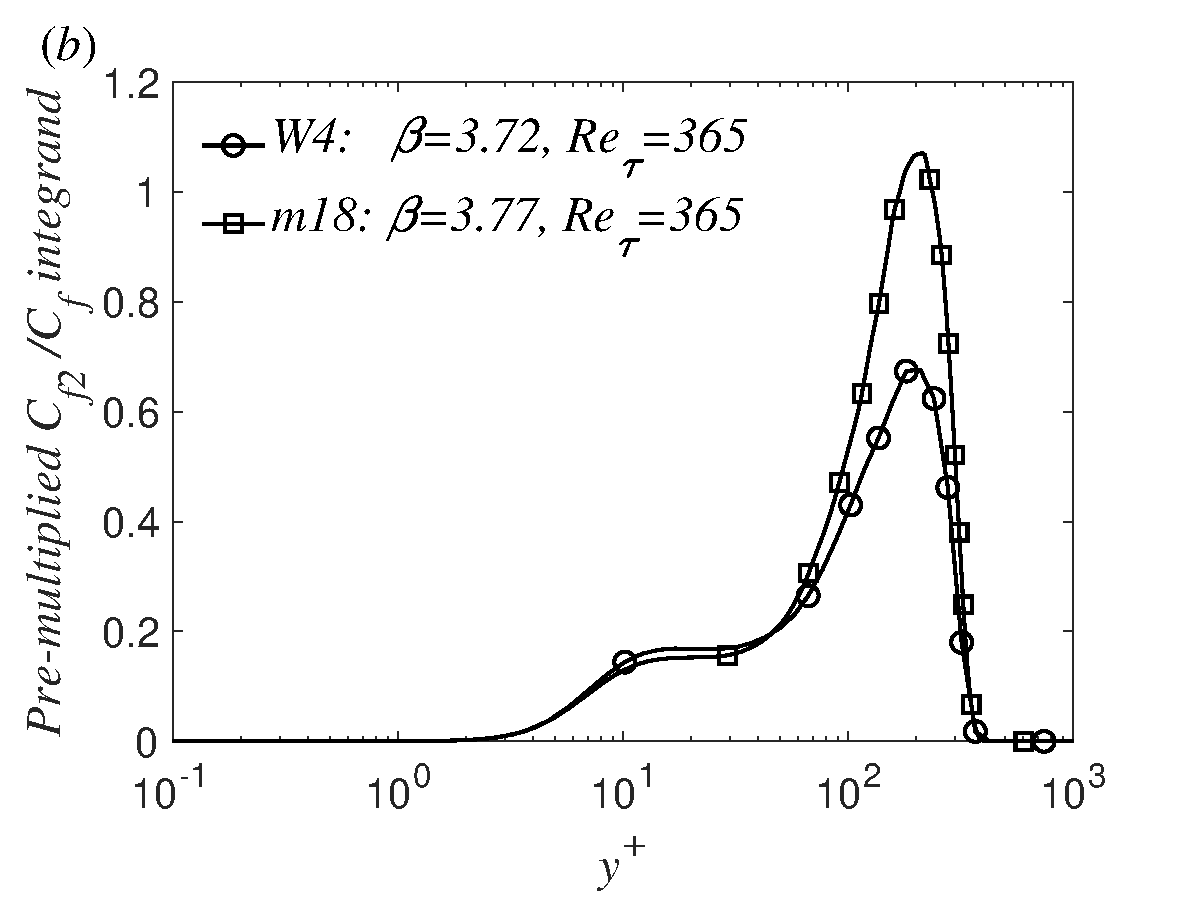
\includegraphics[width = 5cm]{12b}}
\subfigure{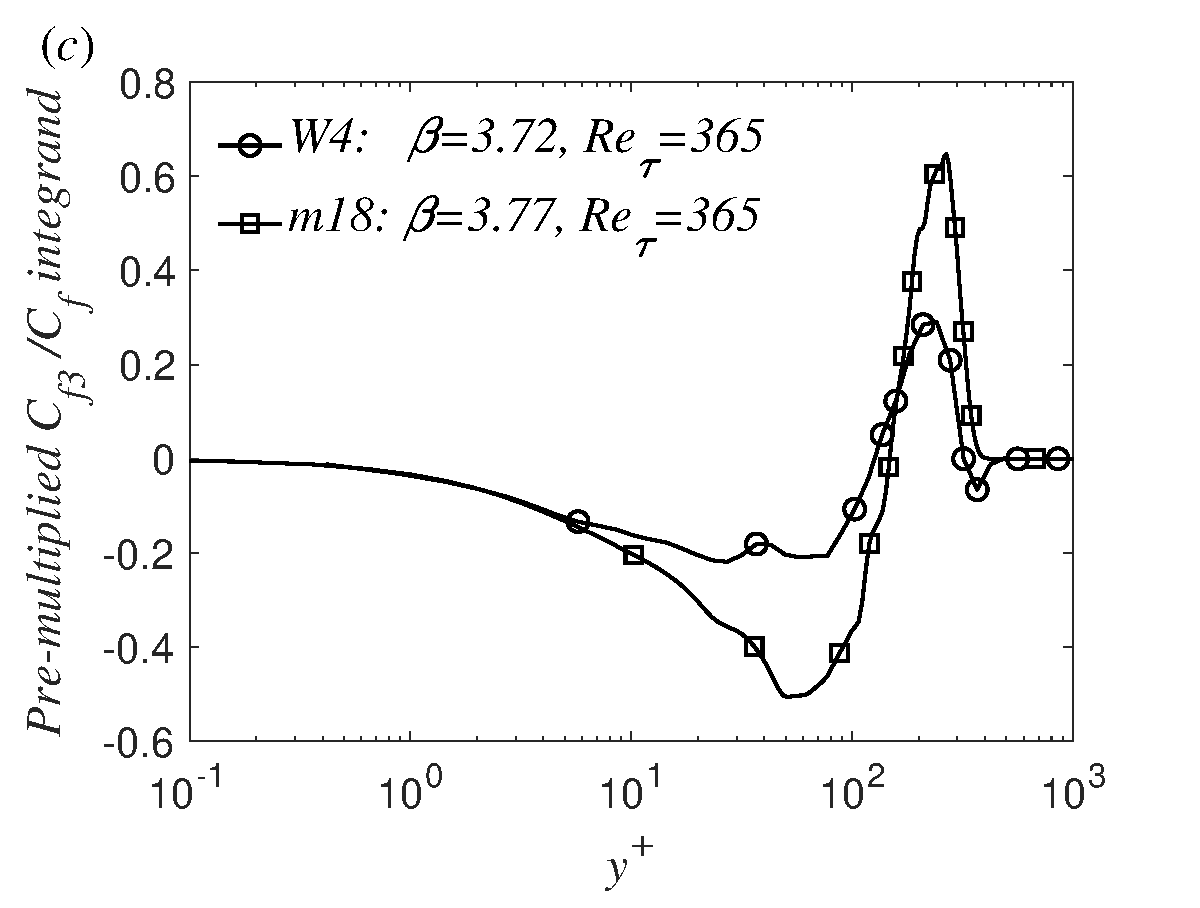
\includegraphics[width = 5cm]{12c}}
\subfigure{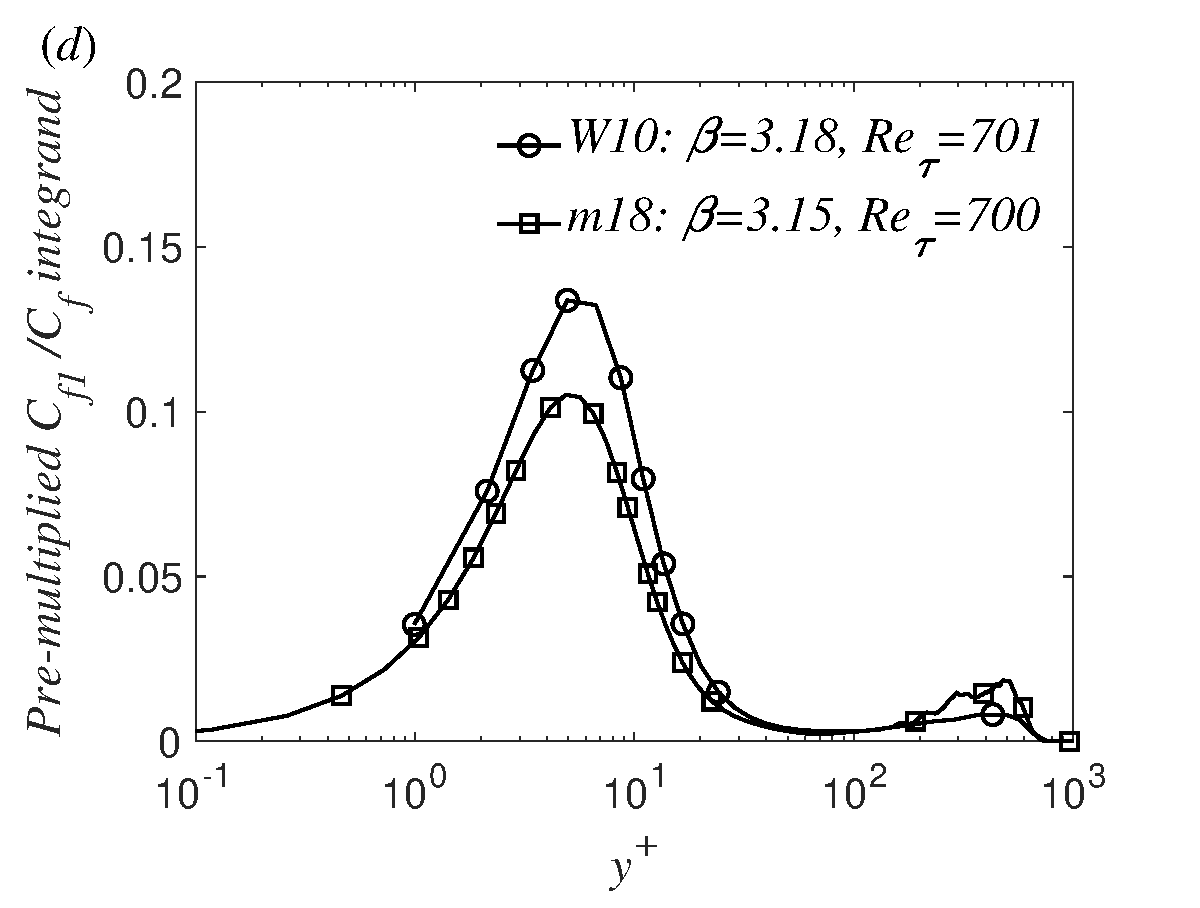
\includegraphics[width = 5cm]{12d}}
\subfigure{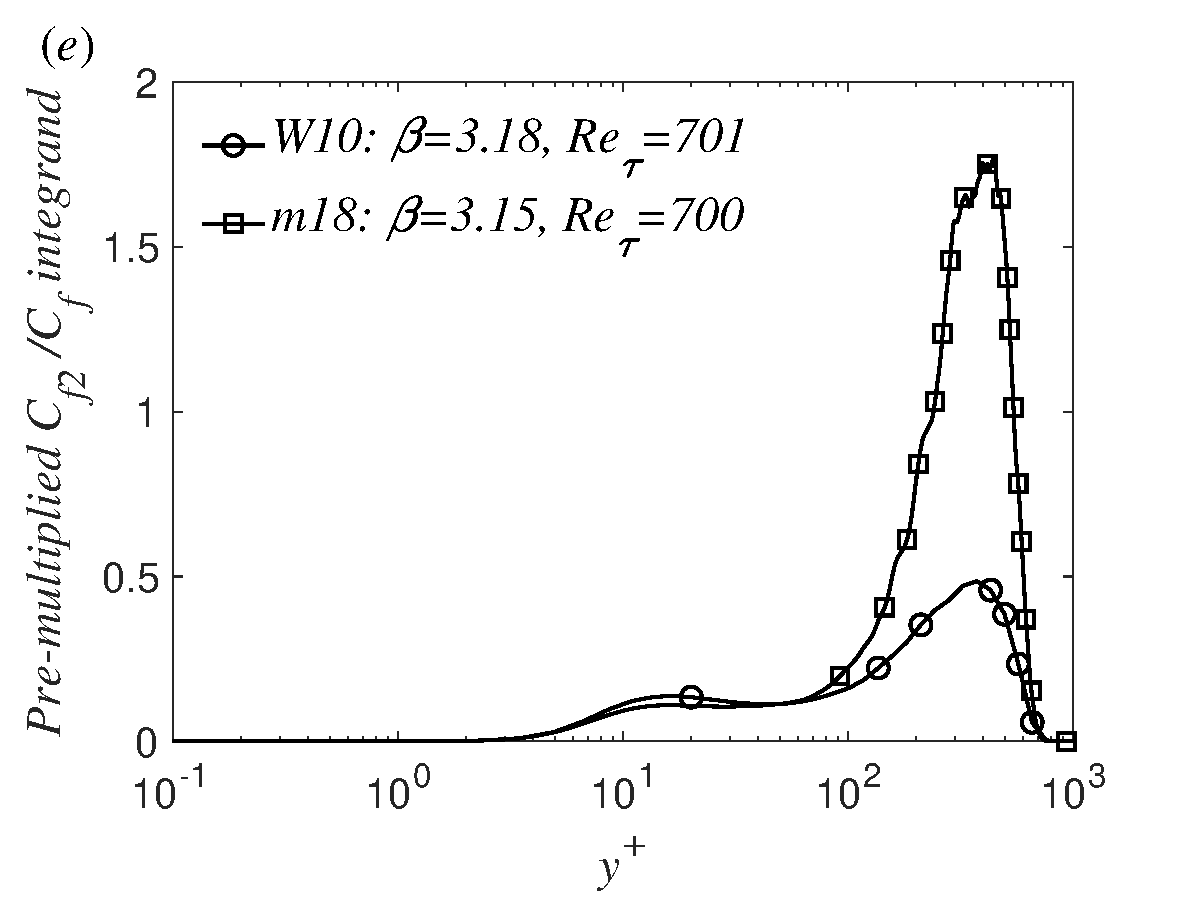
\includegraphics[width = 5cm]{12e}}
\subfigure{\includegraphics[width = 5cm]{12f}}
\subfigure{\includegraphics[width = 5cm]{12g}}
\subfigure{\includegraphics[width = 5cm]{12h}}
\subfigure{\includegraphics[width = 5cm]{12i}}
\caption{Distribution of the pre-multiplied integrand in $C_{f1}/C_f$($a$, $d$, $g$), $C_{f2}/C_f$ ($b$, $e$, $h$), and $C_{f3}/C_f$ ($c$, $f$, $i$) as a function of $y^+$ for the airfoil TBLs for cases $P_1$ ($a$--$c$), $P_2$ ($d$--$f$), and $P_3$ ($g$--$i$).}
\label{history}
\end{figure}






\section{Conclusions}\label{conclusion}

The mean friction drag in adverse-pressure-gradient turbulent boundary layers, developing both on flat-plates and airfoils, has been decomposed with the RD identity\cite{Renard2016}. 
Results show that as the pressure-gradient coefficient $\beta$ increases, the component of direct viscous dissipation ($C_{f1}/C_f$) decreases, and the component of turbulence kinetic energy production ($C_{f2}/C_f$) increases dramatically and becomes dominant for the friction-drag generation. 
By checking the wall-normal distributions of the pre-multiplied integrands in the components, we found that the inner peaks of the $C_{f1}$- and $C_{f2}$-contributions are fixed at $y^+\approx6$ and $y^+\approx16.5$, respectively, and their outer peaks are located at $y/\delta_{99}\approx0.7$ and $y/\delta_{99}\approx0.53$, respectively, regardless of the friction Reynolds number ($Re_\tau$), the magnitude of $\beta$ and its development history. Importantly, stronger accumulated $\beta$ leads to a more pronounced outer-layer contribution to the mean friction drag whereas it reduces the role of inner-layer dynamics.
The component of spatial growth of the flow ($C_{f3}/C_f$) becomes negative in the investigated APG-TBLs and increases with $\beta$. 
Its wall-normal distributions of the pre-multiplied integrand are only well-collapsed in the outer scale.
Furthermore, inner-outer scale separations are more evident in the APG-TBLs than in the ZPG-TBL, even at relatively low Reynolds numbers with the enhancement of outer-scale motions. This leads to significantly larger contributions of outer-layer dissipation,  production and convection, although the pressure gradient itself produces negative contributions.
These observations may help to design promising drag-reduction approaches for the adverse-pressure-gradient turbulent boundary layers.


%This paper separately investigates the effects of two complementary mechanisms, i.e. APG and Reynolds-number variation, on the generation of the skin friction, showing the spatial contribution within the boundary layer.
%Similar to the effect of Reynolds-number increase in the ZPG-TBL, the presence of APG dramatically highlights the importance of outer region especially in terms of the contribution of turbulence kinetic energy production, suggesting a promising skin-friction reduction strategy based on the nature of outer-layer dynamics and turbulence kinetic energy production in adverse-pressure-gradient turbulent boundary layers.

%From the perspective of energy budget, the generation of skin friction is split into three components, respectively associated with direct viscous dissipation ($C_{f1}$), turbulence kinetic energy production ($C_{f2}$), and the spatial growth of the flow ($C_{f3}$). 
%Thereinto, the contribution of $C_{f3}$ can be further decomposed, in terms of flow convection ($C_{f31}$), streamwise heterogeneity ($C_{f32}$) (which is completely negligible at least for the cases under scrutiny), and pressure gradient ($C_{f33}$).
%

%The results have shown that
%
%(1)
%
%as the pressure-gradient coefficient $\beta$ increases, the contribution of $C_{f1}$ decreases while that of $C_{f2}$ dramatically increases. As for $C_{f3}/C_f$, it becomes negative at the presence of adverse pressure gradient at least when $\beta\ge 1$, mainly due to the imposed positive ${\rm d}p/{\rm d}x$, and this negative contribution increases with $\beta$. 
%In the wall-normal distributions of pre-multiplied integrands in $C_{f1}/C_f$, $C_{f2}/C_f$, and $C_{f3}/C_f$, findings are summarized as follows.
%
%
%(2)
%
%$\bullet$~Regardless of the pressure-gradient coefficient and the Reynolds number, the inner peaks of the $C_{f1}$- and $C_{f2}$-contributions are fixed at $y^+\approx6$ and $y^+\approx16.5$, respectively; while their outer peaks are well-scaled by the outer scale at $y/\delta_{99}\approx0.7$ and $y/\delta_{99}\approx0.53$. Both the valley and peak of the
%$C_{f3}$-contributions are also well-collapsed in outer scale at $y/\delta_{99}\approx0.1$ and $y/\delta_{99}\approx0.65$, respectively. 
%
%
%
%
%
%$\bullet$~At the same Reynolds number, the increase of $\beta$ induces the reduction of the inner-layer contribution to the skin-friction generation, whereas significantly amplifies the contribution of $C_{f1}$, $C_{f2}$, and $C_{f3}$ in the outer region owing to the energy enhancement. 
%When increasing the Reynolds number at a same $\beta$, the outer-layer peak values of $C_{f1}$-, $C_{f2}$- and $C_{f3}$-contributions attenuate, indicating the less sensitivity of the higher-$Re$ TBLs to APG effects.
%
%(3)
%
%$\bullet$~Different development histories of the pressure gradient cause the redistribution of the friction contributions along the wall-normal direction. The upstream pressure gradient can be accumulated and the stronger accumulated $\beta$ leads to a more pronounced outer-layer contribution to skin-friction drag whereas reduces the role of inner-layer dynamics.
%
\section*{Acknowledgments}  
The funding support of National Natural Science Foundation of China (under the grant No. 11772194 and 91952302) is acknowledged.  Ricardo Vinuesa also acknowledges support from the Swedish Research Council (VR). 
{\color{black}
The authors gratefully acknowledge a comment by a reviewer of this article, which gives us a clue to explain the independence of the peak locations from a mathematical point of view.}


\renewcommand\thefigure{\Alph{section}\arabic{figure}}    
\setcounter{figure}{0}   


\appendix


\section{Decomposed constituents in flat-plate APG-TBLs for $\beta\approx1$ and 2}\label{app1}

Figures~\ref{app:fig1} and \ref{app:fig2} quantify the wall-normal distributions of the pre-multiplied integrands in $C_{f1}/C_f$, $C_{f2}/C_f$, and $C_{f3}/C_f$ in equations \eqref{cf1_cf}-\eqref{cf3_cf} , for $\beta\approx1$ and 2 respectively, with $Re_\tau$ ranging from 400 to 750.
%Figure~\ref{app:fig2} plots the pre-multiplied distributions of the $C_f^{2/3}$-scaled $C_{f1}$ and $C_{f2}$ as a function of $y^+$ at $\beta\approx2$.
The conclusions regarding Reynolds-number effects discussed in Sec. \ref{Re-eff} at higher Reynolds number are confirmed here.

\begin{figure}[htb]
\subfigure{\includegraphics[width = 5cm]{13a} }
\subfigure{\includegraphics[width = 5cm]{13b} }
\subfigure{\includegraphics[width = 5cm]{13c} }
\subfigure{\includegraphics[width = 5cm]{13d} }
\subfigure{\includegraphics[width = 5cm]{13e} }
\subfigure{\includegraphics[width = 5cm]{13f} }
\caption{Distributions of the pre-multiplied integrand in $C_{f1}/C_f$ ($a$, $d$), $C_{f2}/C_f$ ($b$, $e$), and $C_{f3}/C_f$ ($c$, $f$) as a function of $y^+$ ($a$--$c$) and as a function of  $y/\delta_{99}$  ($d$--$f$)  for the APG-TBL with $\beta\approx1$. The vertical dashed lines in ($d$--$f$) mark the position $y/\delta_{99}=0.7$, 0.53, and 0.65 respectively.}
\label{app:fig1}
\end{figure}

\begin{figure}[htb]
\subfigure{\includegraphics[width = 5cm]{14a} }
\subfigure{\includegraphics[width = 5cm]{14b} }
\subfigure{\includegraphics[width = 5cm]{14c} }
\subfigure{\includegraphics[width = 5cm]{14d} }
\subfigure{\includegraphics[width = 5cm]{14e} }
\subfigure{\includegraphics[width = 5cm]{14f} }
\caption{Distributions of the pre-multiplied integrand in $C_{f1}/C_f$ ($a$, $d$), $C_{f2}/C_f$ ($b$, $e$), and $C_{f3}/C_f$ ($c$, $f$) as a function of $y^+$ ($a$--$c$) and as a function of  $y/\delta_{99}$  ($d$--$f$)  for the APG-TBL with $\beta\approx2$. The vertical dashed lines in ($d$--$f$) mark the position $y/\delta_{99}=0.7$, 0.53, and 0.65 respectively.}
\label{app:fig2}
\end{figure}

\iffalse
\begin{figure}
\subfigure{\includegraphics[width = 8cm]{fig/b2_disp15}}
\subfigure{\includegraphics[width = 8cm]{fig/b2_prop15}}
\caption{The distributions of the pre-multiplied integrand in ($a$) $C_{f1}/C_f^{3/2}$ and ($b$) $C_{f2}/C_f^{3/2}$, as a function of $y^+$ for the TBLs at $\beta\approx2$. (For the legends, see figure \ref{app:fig1}.)}
\label{app:fig3}
\end{figure}
\fi



% \bibliographystyle{unsrtnat}
% \bibliography{pressure_gradient}



% \end{document}

